\chapter{Results}
\label{cha:results}

In this chapter the results generated with the open source tool are presented.
This chapter is divided into two sections.
Section \ref{sec:results_verification} presents results from previous papers recreated using the tool.
Section \ref{sec:results_new} presents results from the newer family of models introduced in \cite{Ferrer2018a}

\section{Verification of previous results}
\label{sec:results_verification}

In this section a replication of previous results is presented.
This allows to verify the model and its implementation against previous experiments.

However, in some cases there was limited information in the original papers about the parameters used in the experiments.
This concerned details regarding the initial graphs and the specifics of the optimization process.
In other cases, there were errors in previous papers.
This was due to undetected programming errors.
In both cases, determining the correct parameter becomes a matter of trial and error.

The $\phi$ parameter was not considered in either of the papers replicated in this section, and so it is set to 0.

Section \ref{sec:results_verification_first} replicates the results from \cite{Ferrer2005a}, which correspond to the \firstmodel{} from this thesis.
Section \ref{sec:results_verification_second} replicates the results from \cite{Ferrer2003a}, corresponding to the \secondmodel{}.

\subsection{Results from the \firstmodel{} (2005)}
\label{sec:results_verification_first}

\begin{figure}
  \addjankysubfigure{a)}{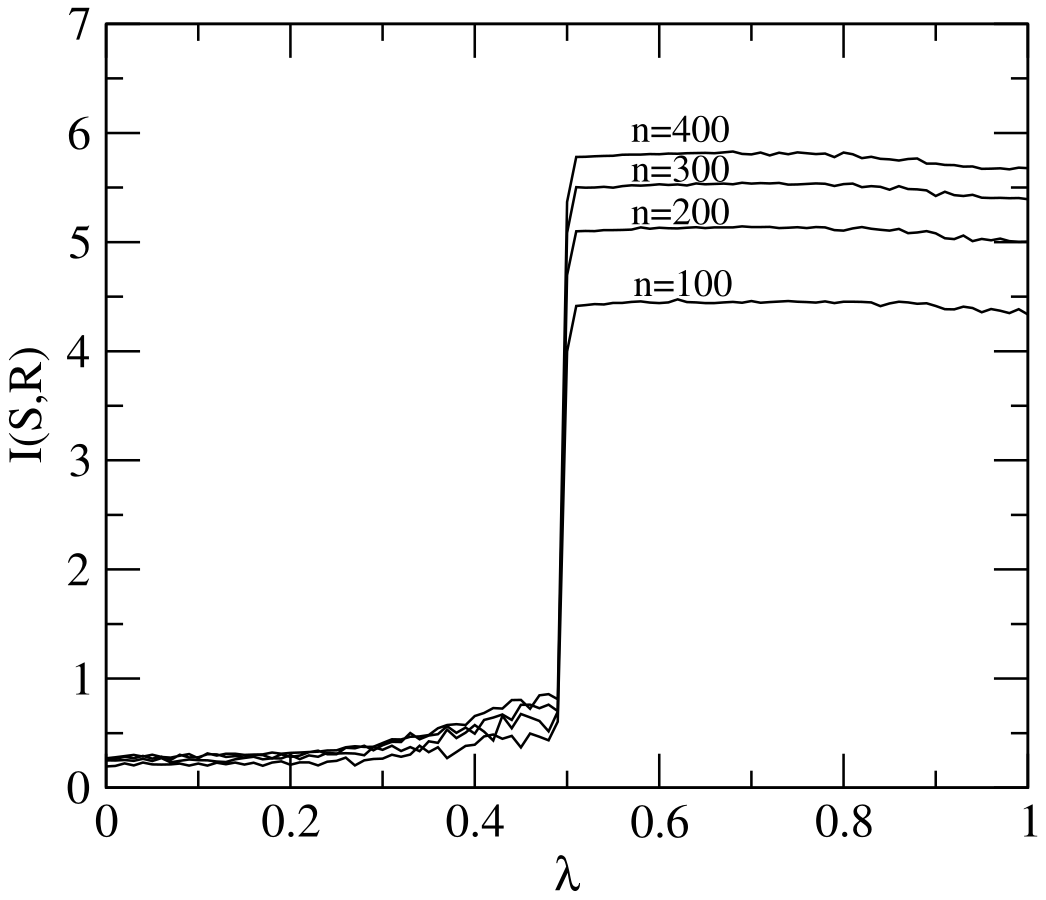
\includegraphics[width=\textwidth,height=.4\textheight,keepaspectratio]{fig2_2005_old}}
  \addjankysubfigure{b)}{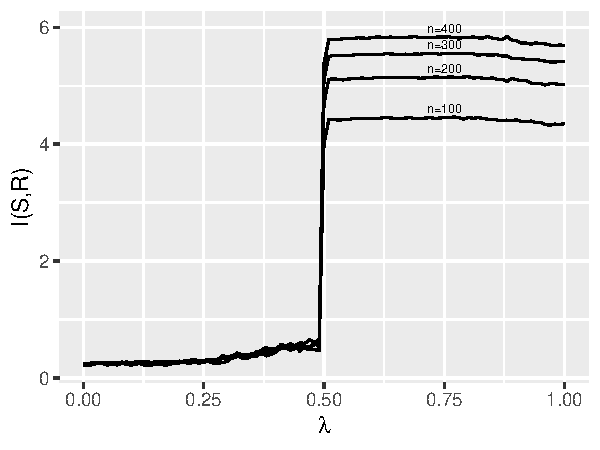
\includegraphics[width=\textwidth,height=.4\textheight,keepaspectratio]{figure2_article_EPJ_B_2005}}
  \caption{
    The mutual information $I(S,R)$ is in the $y$ axis and the $\lambda$ parameter on the $x$ axis.
    Graphs of different sizes are shown, $n=m=100$, $n=m=200$, $n=m=300$, $n=m=400$.
    Averages over 30 realizations.
    $\phi=0$, the initial graph is $G_{n,m,1/n}$, each iteration of the optimization algorithm performs 2 mutations on the graph, the weak stop condition is used to stop the optimization process, unlinked objects are allowed.\\
    Subfigure a corresponds with Figure 2 from \cite{Ferrer2005a}.\\
    Subfigure b is the recreation of that same figure.
  }
  \label{fig:fig2_2005}
\end{figure}

\begin{figure}
  \addjankysubfigure{a)}{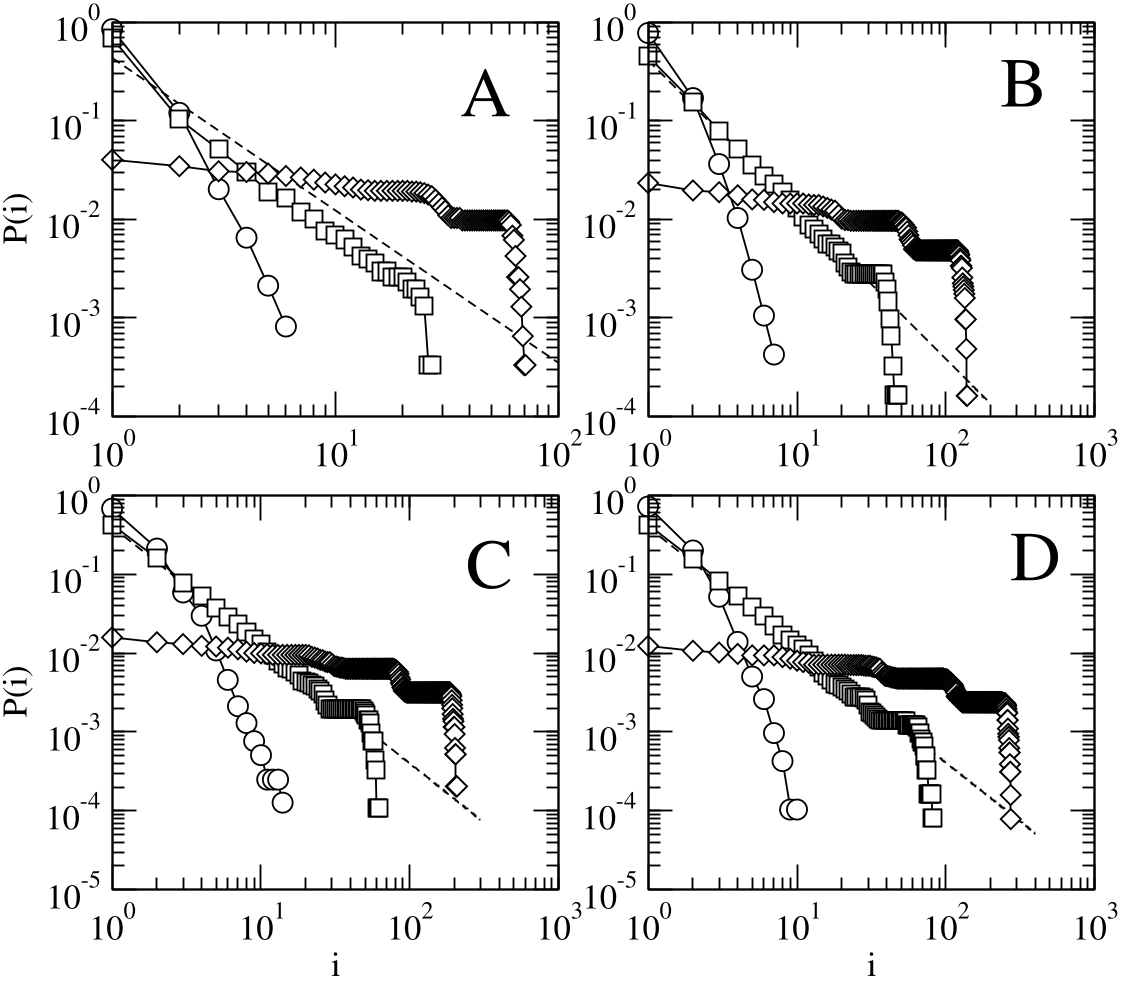
\includegraphics[width=\textwidth,height=.35\textheight,keepaspectratio]{fig3_2005_old}}
  \addjankysubfigure{b)}{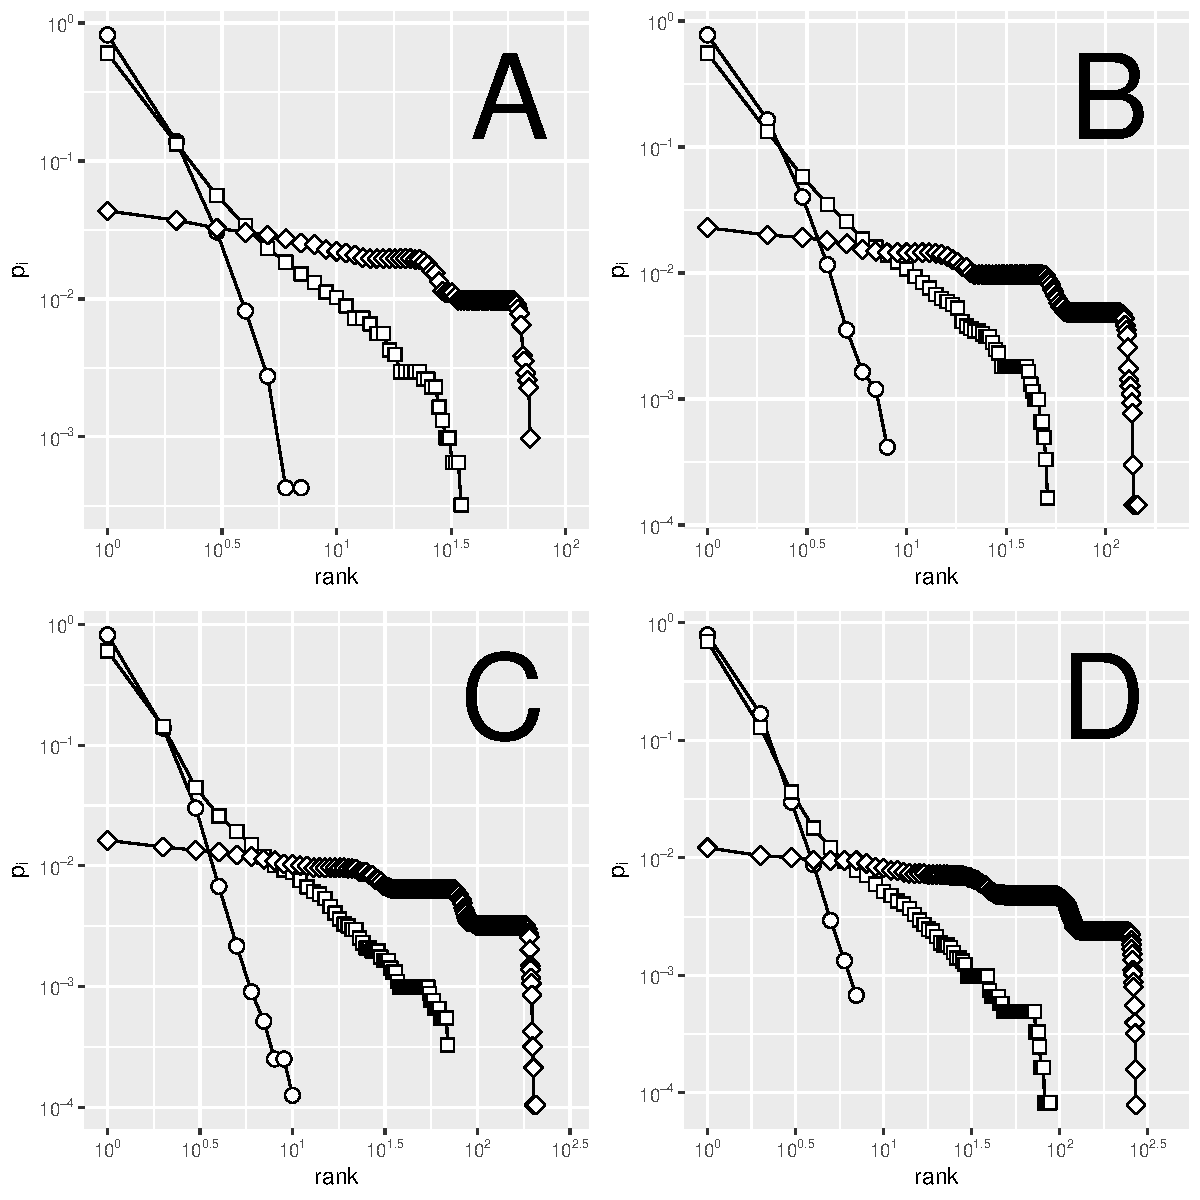
\includegraphics[width=\textwidth,height=.35\textheight,keepaspectratio]{figure3_article_EPJ_B_2005}}
  \caption{
    $P(i)$, the probability of the $i$th most frequent signal, obtained from minimum energy configurations for systems of sizes $n=m=100$ (A), $n=m=200$ (B), $n=m=300$ (C), $n=m=400$ (D).
    Four series are shown in each plot, $\lambda=0.49$ (circles), $\lambda=\lambda^*$ (squares) and $\lambda=0.5$ (diamonds) and the ideal curve for $\alpha^*$.
    Averages over 30 realizations.
    When $\lambda=\lambda^*$, $\alpha^* = 1.54$ for $n=m=100$, $\alpha^* = 1.51$ for $n=m=200$, $\alpha^* = 1.5$ for $n=m=300$ and $\alpha^* = 1.49$ for $n=m=400$.
    It was chosen that $\lambda^* = 0.4986$ for $n=m=100$, $\lambda^* = 0.4987$ for $n=m=200$, $\lambda^* = 0.4987$ for $n=m=300$, and $\lambda^* = 0.4986$ for $n=m=400$.
    Averages over 30 realizations.
    $\phi=0$, the initial graph is $G_{n,m,1/n}$, each iteration of the optimization algorithm performs 2 mutations on the graph, the weak stop condition is used to stop the optimization process, unlinked objects are allowed.\\
    Subfigure a corresponds with Figure 3 from \cite{Ferrer2005a}.\\
    Subfigure b is the recreation of that same figure.
  }
  \label{fig:fig3_2005}
\end{figure}

Figure \ref{fig:fig2_2005} shows both the original Figure 2 from \cite{Ferrer2005a} and a recreation of this figure using the new tool.
Figure \ref{fig:fig3_2005} shows both the original Figure 3 from \cite{Ferrer2005a} and a recreation of this figure, also generated using the new tool.

The initial graph was not specified in \cite{Ferrer2005a} and a $G_{n,m,1/n}$ ($n=m$) graph is used in the replication.
The paper also does not specify how to stop the optimization process and so the weak stop condition (Section \ref{sec:methods_optimization}) is used.

Subfigures a and b from Figure \ref{fig:fig2_2005} are nearly identical.
In Figure \ref{fig:fig3_2005}, subfigures a and b are also qualitatively very similar.
Although some of the points can be seen to be not quite in the same place.

\subsection{Results from the \secondmodel{} (2003)}
\label{sec:results_verification_second}

\begin{figure}
  \addjankysubfigure{a)}{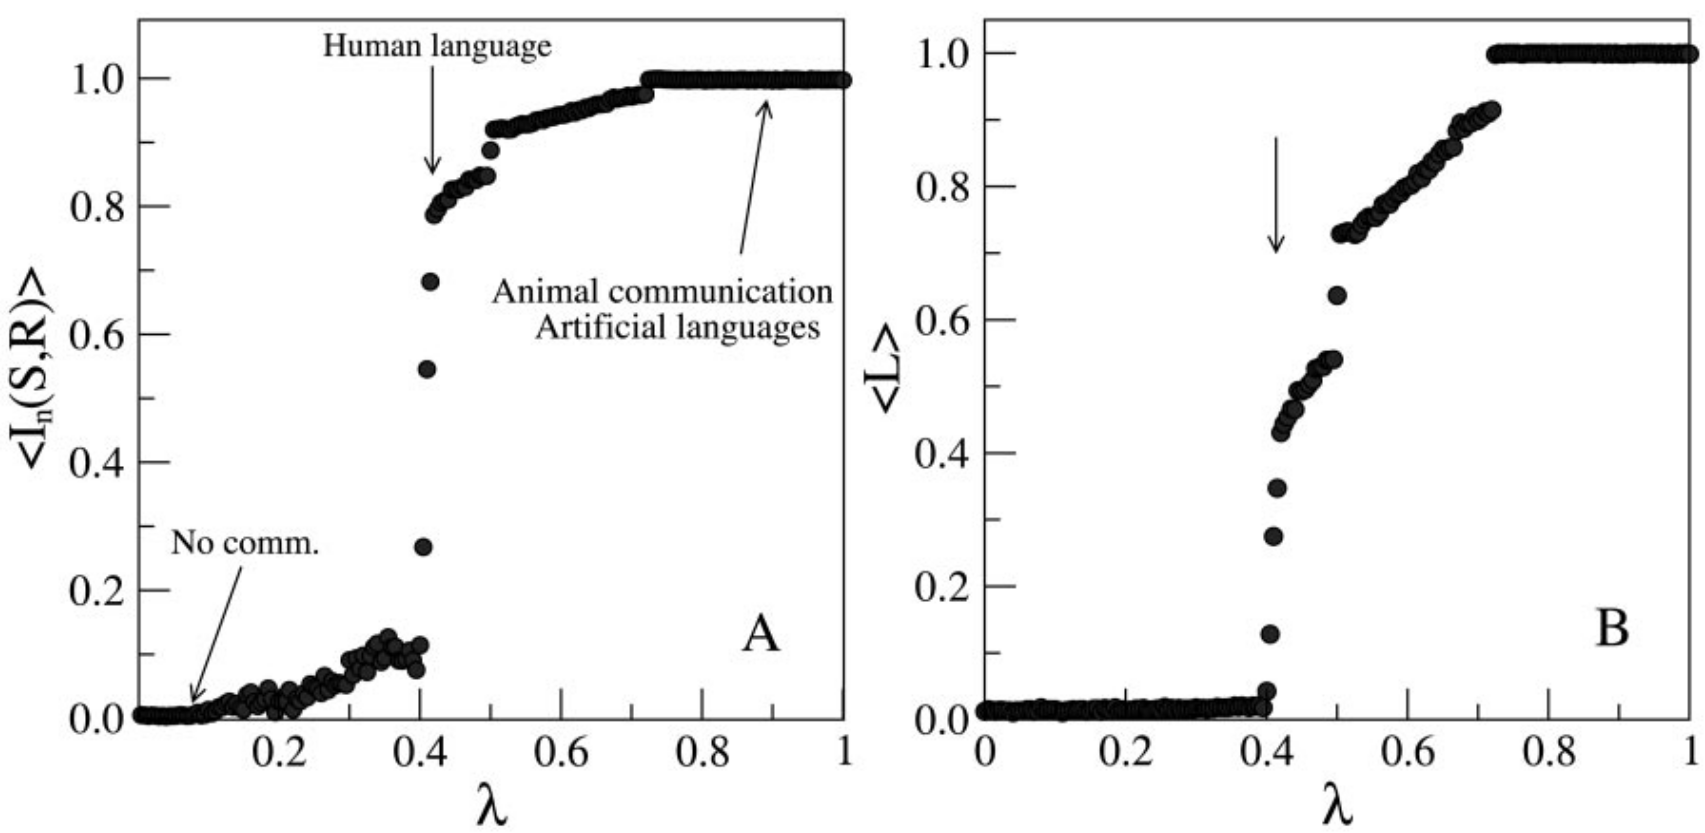
\includegraphics[width=\textwidth]{fig2_2003_old}}
  \addjankysubfigure{b)}{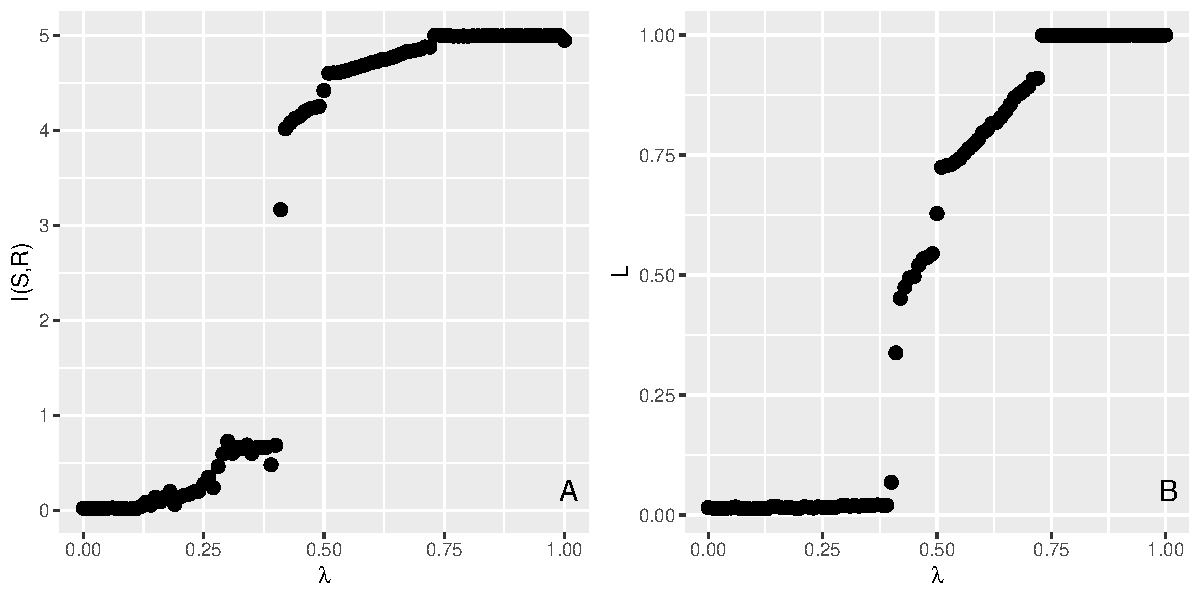
\includegraphics[width=\textwidth]{figure2_article_PNAS_2003_binom1.75}}
  \caption{
    In A, $I(S,R)$ is the mutual information obtained for values of $\lambda$ between 0 and 1.
    In B, $L$ is the lexicon size obtained for values of $\lambda$ between 0 and 1.
    An abrupt change is seen for $\lambda \approx 0.41$ in both A and B.
    Averages over 30 replicas.
    $n=m=150$, $\phi=0$, unlinked objects are not allowed, $\pi$ follows a uniform distribution.\\
    Subfigure a corresponds with Figure 2 from \cite{Ferrer2003a}\\
    Subfigure b is the recreation of that same figure using the open source tool created for this thesis.
  }
  \label{fig:fig2_2003}
\end{figure}

\begin{figure}
  \addjankysubfigure{a)}{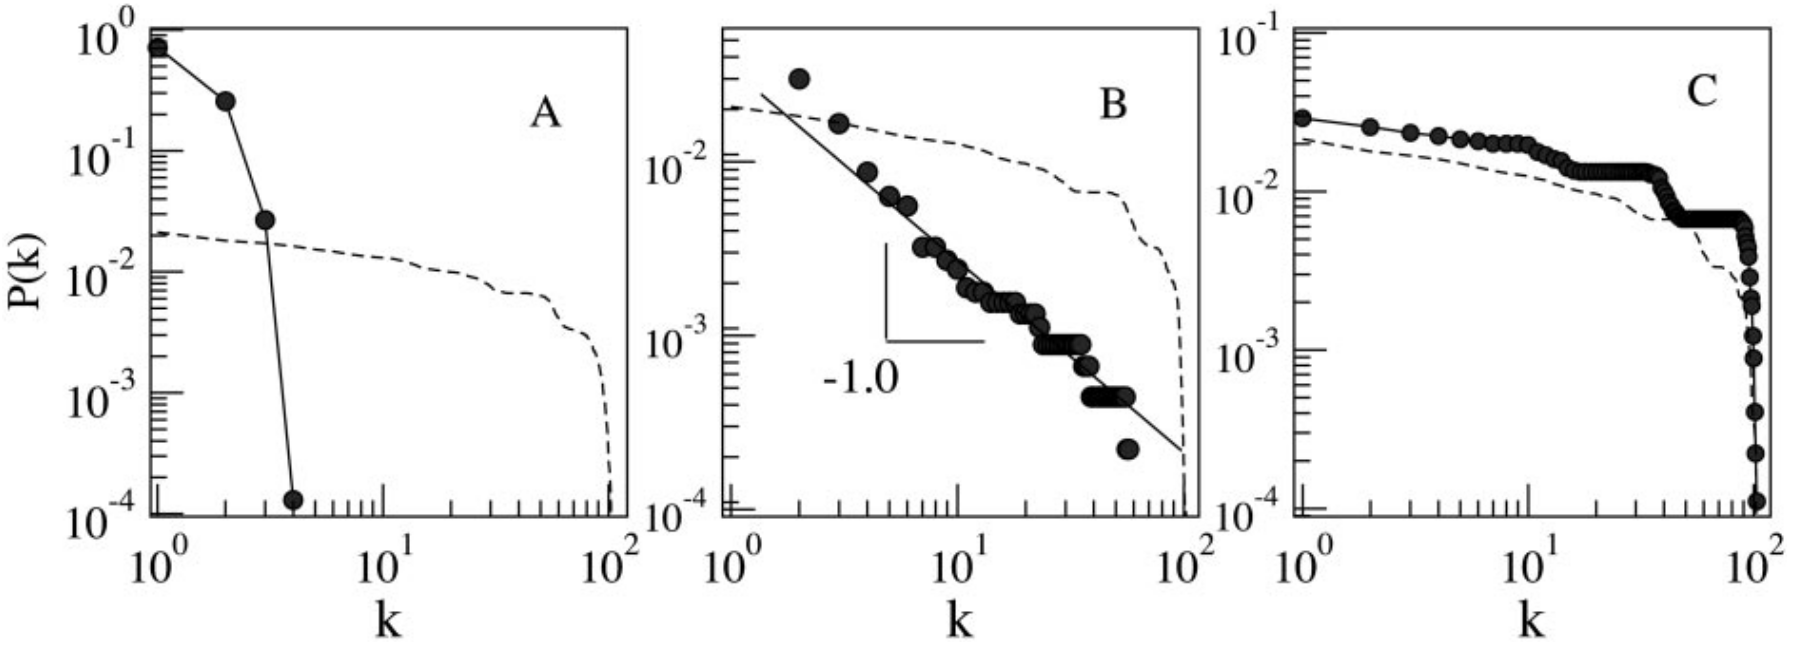
\includegraphics[width=\textwidth]{fig3_2003_old}}
  \addjankysubfigure{b)}{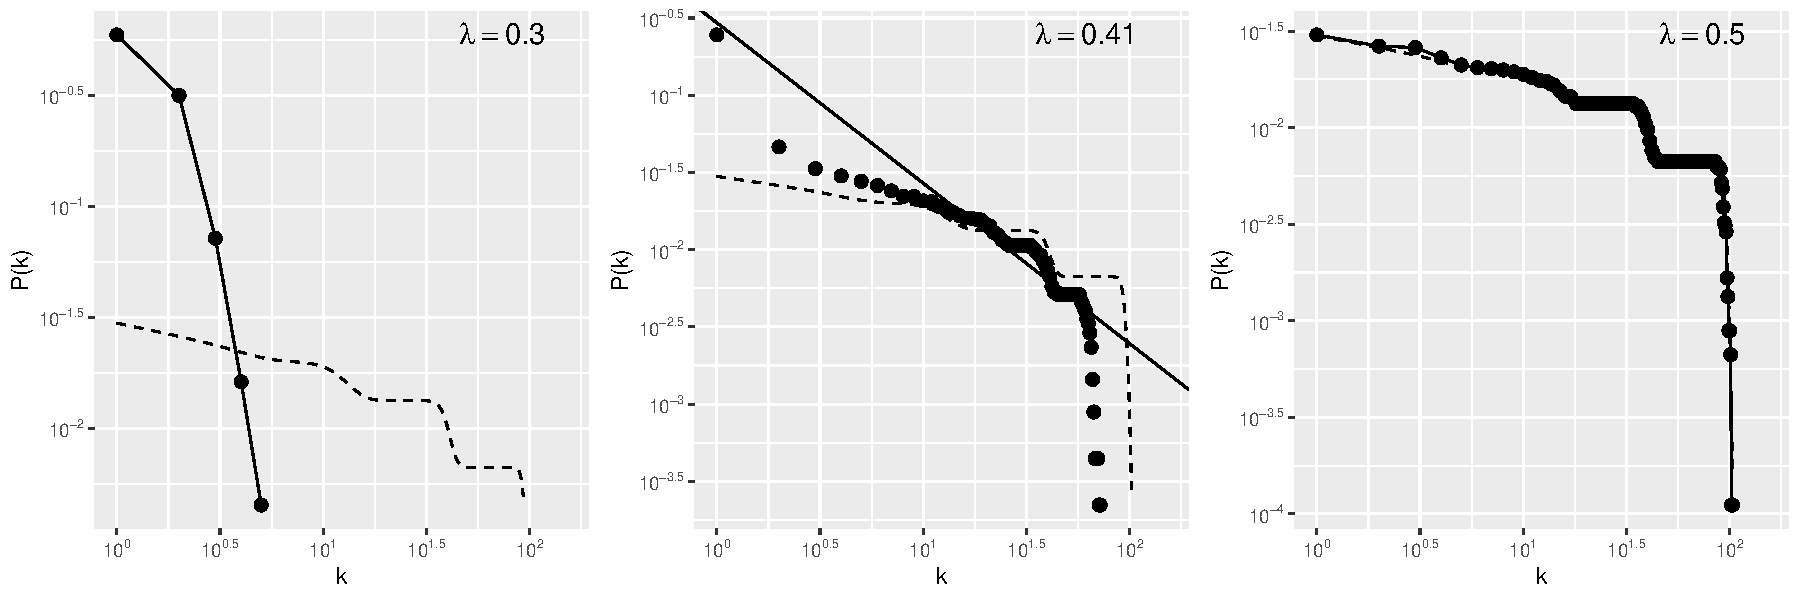
\includegraphics[width=\textwidth]{figure3_article_PNAS_2003_binom1.75}}
  \caption{
    Normalized signal frequency $P(k)$ versus rank $k$.
    The dashed lines show the distribution obtained when from a $G_{n,m,e^*}$ graph where $e^*$ is the number of connections in these optimal configurations.
    In both cases the distribution of B is still consistent with human language, $\alpha=1$.
    Averages over 30 replicas, $n=m=150$, the initial graph is $G_{n,m,10/n}$, the number of mutations on each iteration follows a binomial distribution with average 1.75, the optimization stops after $2nm$ mutations that do not improve the cost function.\\
    Above: Figure 3 from \cite{Ferrer2003a}\\
    Below: Recreation of that same figure using the open source tool created for this thesis.
  }
  \label{fig:fig3_2003}
\end{figure}

Figure \ref{fig:fig2_2003} shows both the original Figure 2 from \cite{Ferrer2003a} and the recreation of this figure using the new tool.
Figure \ref{fig:fig3_2003} shows the original Figure 3 from \cite{Ferrer2003a} and a recreation using the new tool.

The initial graph was specified as a $G_{n,m,\rho}$ but the value of $\rho$ was not given in the paper, a $G_{n,m,10/n}$ graph was used (that is, a value of $\rho=\frac{10}{n}$).
It is specified that the number of mutations done on each iteration of the optimization algorithm follows a binomial distribution.
However it was later found that, due to a bug in the generator of binomial numbers, the number of mutations must have been lower.
Several values were tried for the average number of binomial mutations, with 1.75 giving the results most similar to the previous model's.

Qualitatively, it seems that the two subfigures in Figure \ref{fig:fig2_2003} are very similar.
Some of the points in A do not form exactly the same shape, however, and it seems that not as many points appear inside the phase transition.
As for Figure \ref{fig:fig3_2003}, subfigures A and C are quite similar (although the dashed line appears to overlap the data in subfigure b more than it did in a).
Subfigure B is not as similar.
However, the slope of the curve is also 1.0 as indicated by the solid line.

\redtxt{TODO: arreglar figura que no queda be i potser canviar A i B perque no entrin en conflicte amb els que ja hi ha a les figures?}

\section{Results for current models}
\label{sec:results_new}

Here new results obtained from the model are presented.
Firstly, and as a way to for an intuition of the kinds of graphs that these models generate, Section \ref{sec:results_new_graph} presents the optimal graphs for different initial conditions for both models.
Section \ref{sec:results_new_other} shows the rest of the obtained results.
This section focuses first on plots of the values obtained for the information theoretical measures of the optimal graphs for various value of $\lambda$ in the cost function.
As a reminder, $\lambda$ controls the weight of either the entropy or the mutual information in the cost function.
Statistical measures for select values of $\lambda$ are then shown.
These measures show how various linguistic laws appear in the results.
Several kinds of initial graphs are shown throughout this section.

\begin{itemize}
\item Random: The initial graph is a $G_{n,m,3/n/m}$ random graph.
\item Single link: The initial graph contains a single link between a word and a meaning.
\item One-to-one: The initial graph is a bijection connecting words and meanings one to one
\item Complete: The initial graph is a complete bipartite graph where every word connects to every meaning and every meaning to every word.
\end{itemize}

All results in this section perform two mutations on each iteration of the optimization algorithm, which stops with the \emph{weak} stop condition.
See Section \ref{sec:methods_optimization} for more information on the optimization process.

\subsection{Graph visualization}
\label{sec:results_new_graph}

Here various graphs are plotted.
These plots all correspond to graphs of size $n=m=60$ and $\phi=1$.
Unlinked meanings are also allowed in all graphs.
It is interesting to see the different shapes the graph takes for different values of $\lambda$.

For the first model, four graphs are shown.

\begin{itemize}
\item Random initial graph, Figure \ref{fig:graphVisualization_firstModel_phi1_nm60_static_randomBipartite_allowUnlinked}.
\item Single link initial graph, Figure \ref{fig:graphVisualization_firstModel_phi1_nm60_static_singleLink_allowUnlinked}.
\item One-to-one initial graph, Figure \ref{fig:graphVisualization_firstModel_phi1_nm60_static_oneToOne_allowUnlinked}.
\item Complete initial graph, Figure \ref{fig:graphVisualization_firstModel_phi1_nm60_static_complete_allowUnlinked}.
\end{itemize}

For the second model, the \emph{a priori} probability $\pi$ follows a uniform distribution.
Four additional graphs are shown.

\begin{itemize}
\item Random initial graph, Figure \ref{fig:graphVisualization_uniform_phi1_nm60_static_randomBipartite_allowUnlinked}
\item Single link initial graph, Figure \ref{fig:graphVisualization_uniform_phi1_nm60_static_singleLink_allowUnlinked}
\item One-to-one initial graph, Figure \ref{fig:graphVisualization_uniform_phi1_nm60_static_oneToOne_allowUnlinked}
\item Complete initial graph, Figure \ref{fig:graphVisualization_uniform_phi1_nm60_static_complete_allowUnlinked}
\end{itemize}

\begin{figure}
  \centering
  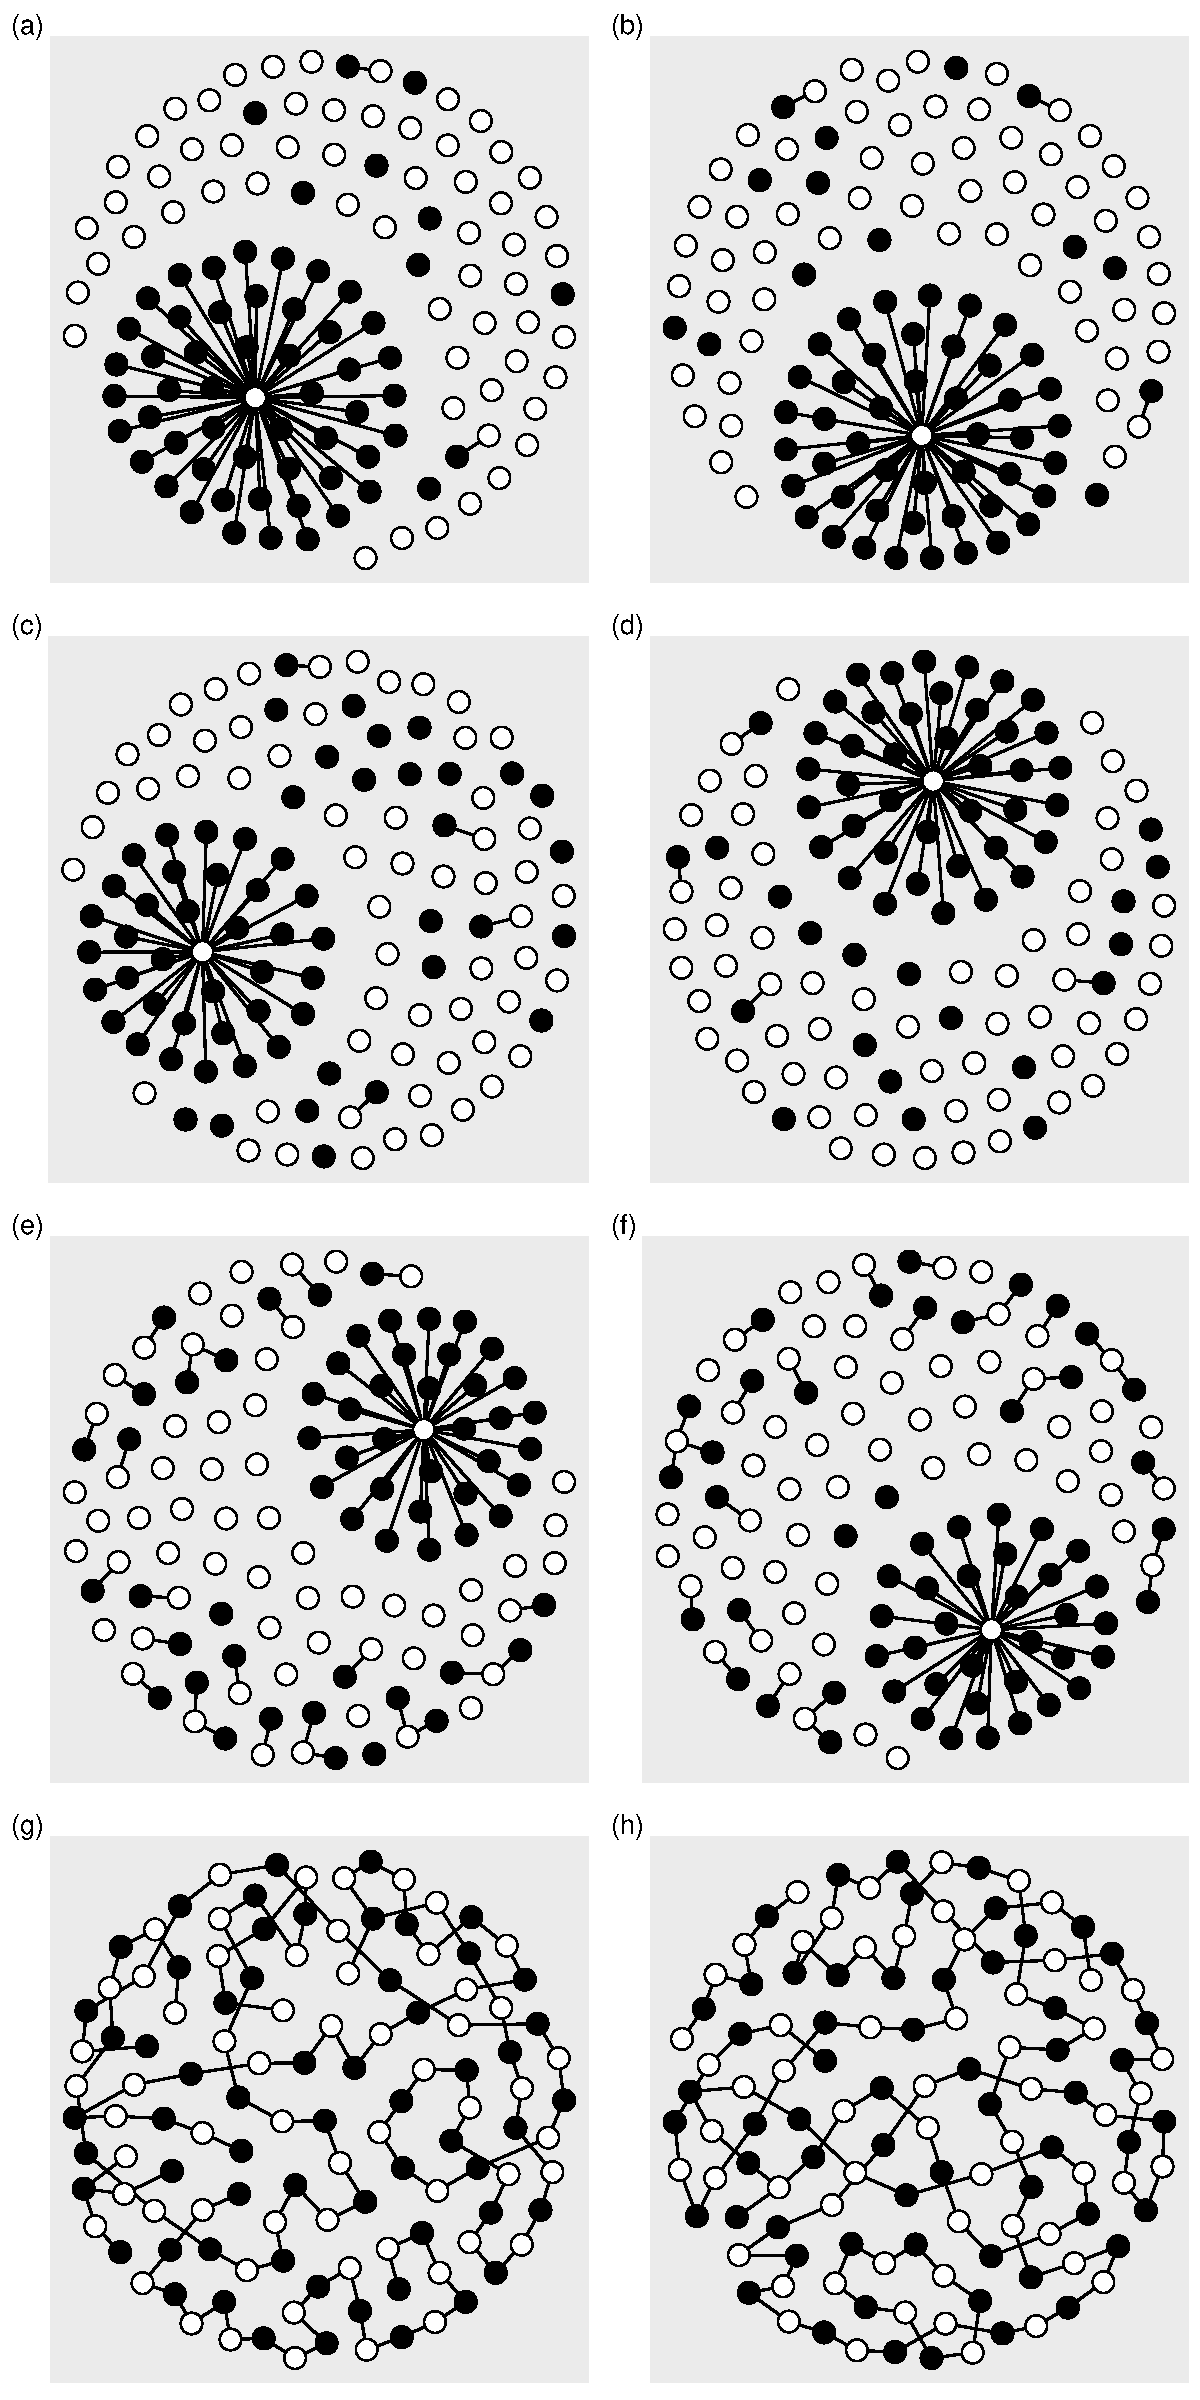
\includegraphics[height=\textheight,width=\textwidth,keepaspectratio]{graphVisualization_firstModel_phi1_nm60_static_randomBipartite_allowUnlinked}
  \caption{a}
  \label{fig:graphVisualization_firstModel_phi1_nm60_static_randomBipartite_allowUnlinked}
\end{figure}

\begin{figure}
  \centering
  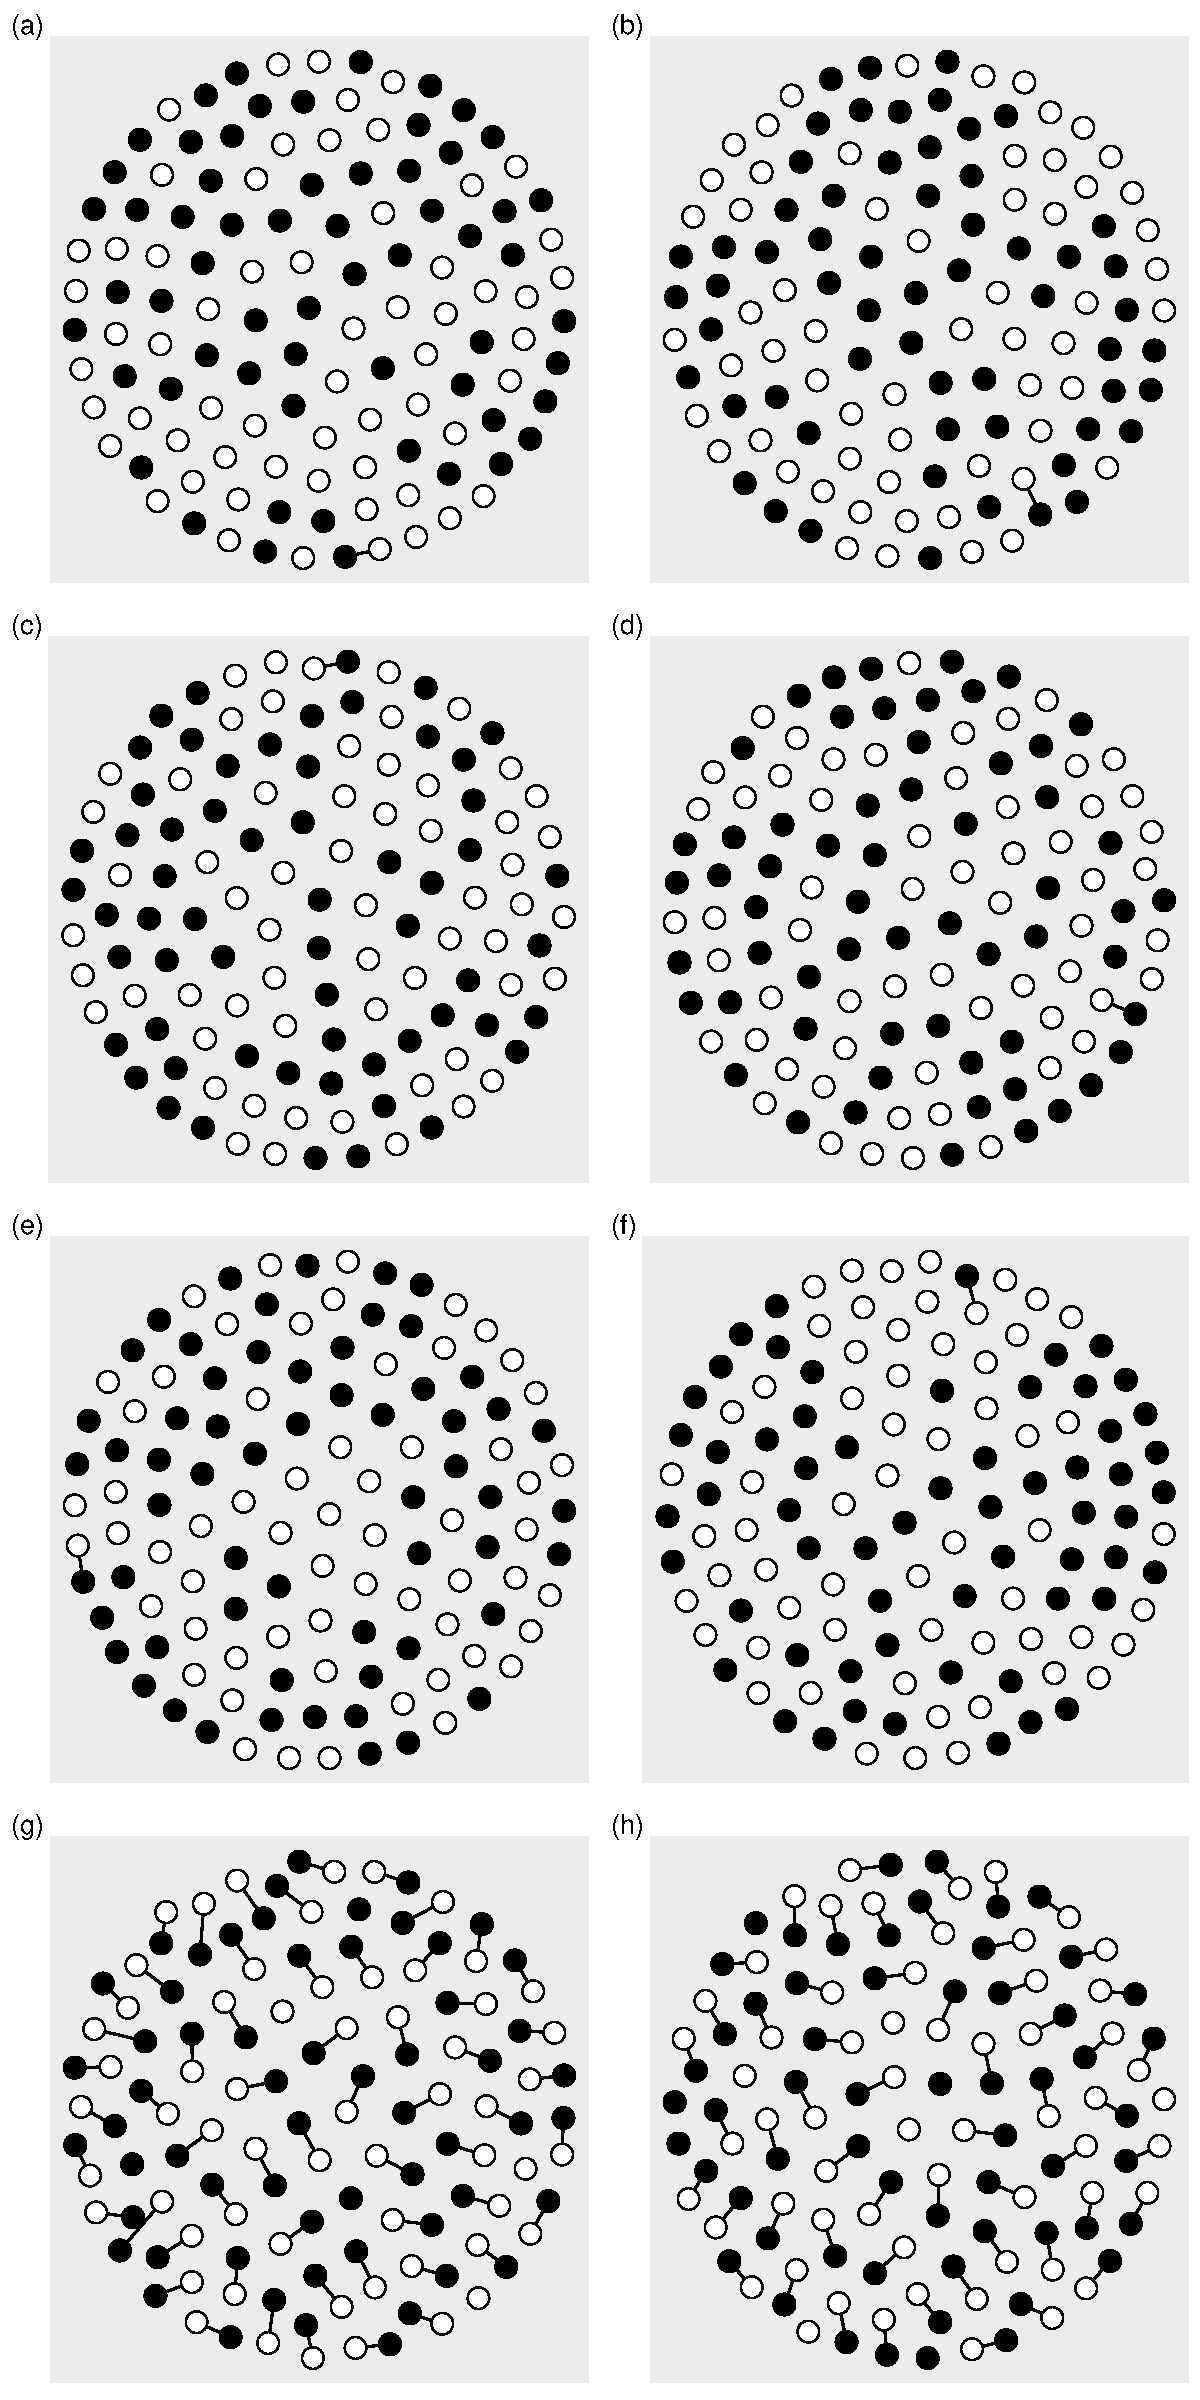
\includegraphics[height=\textheight,width=\textwidth,keepaspectratio]{graphVisualization_firstModel_phi1_nm60_static_singleLink_allowUnlinked}
  \caption{a}
  \label{fig:graphVisualization_firstModel_phi1_nm60_static_singleLink_allowUnlinked}
\end{figure}

\begin{figure}
  \centering
  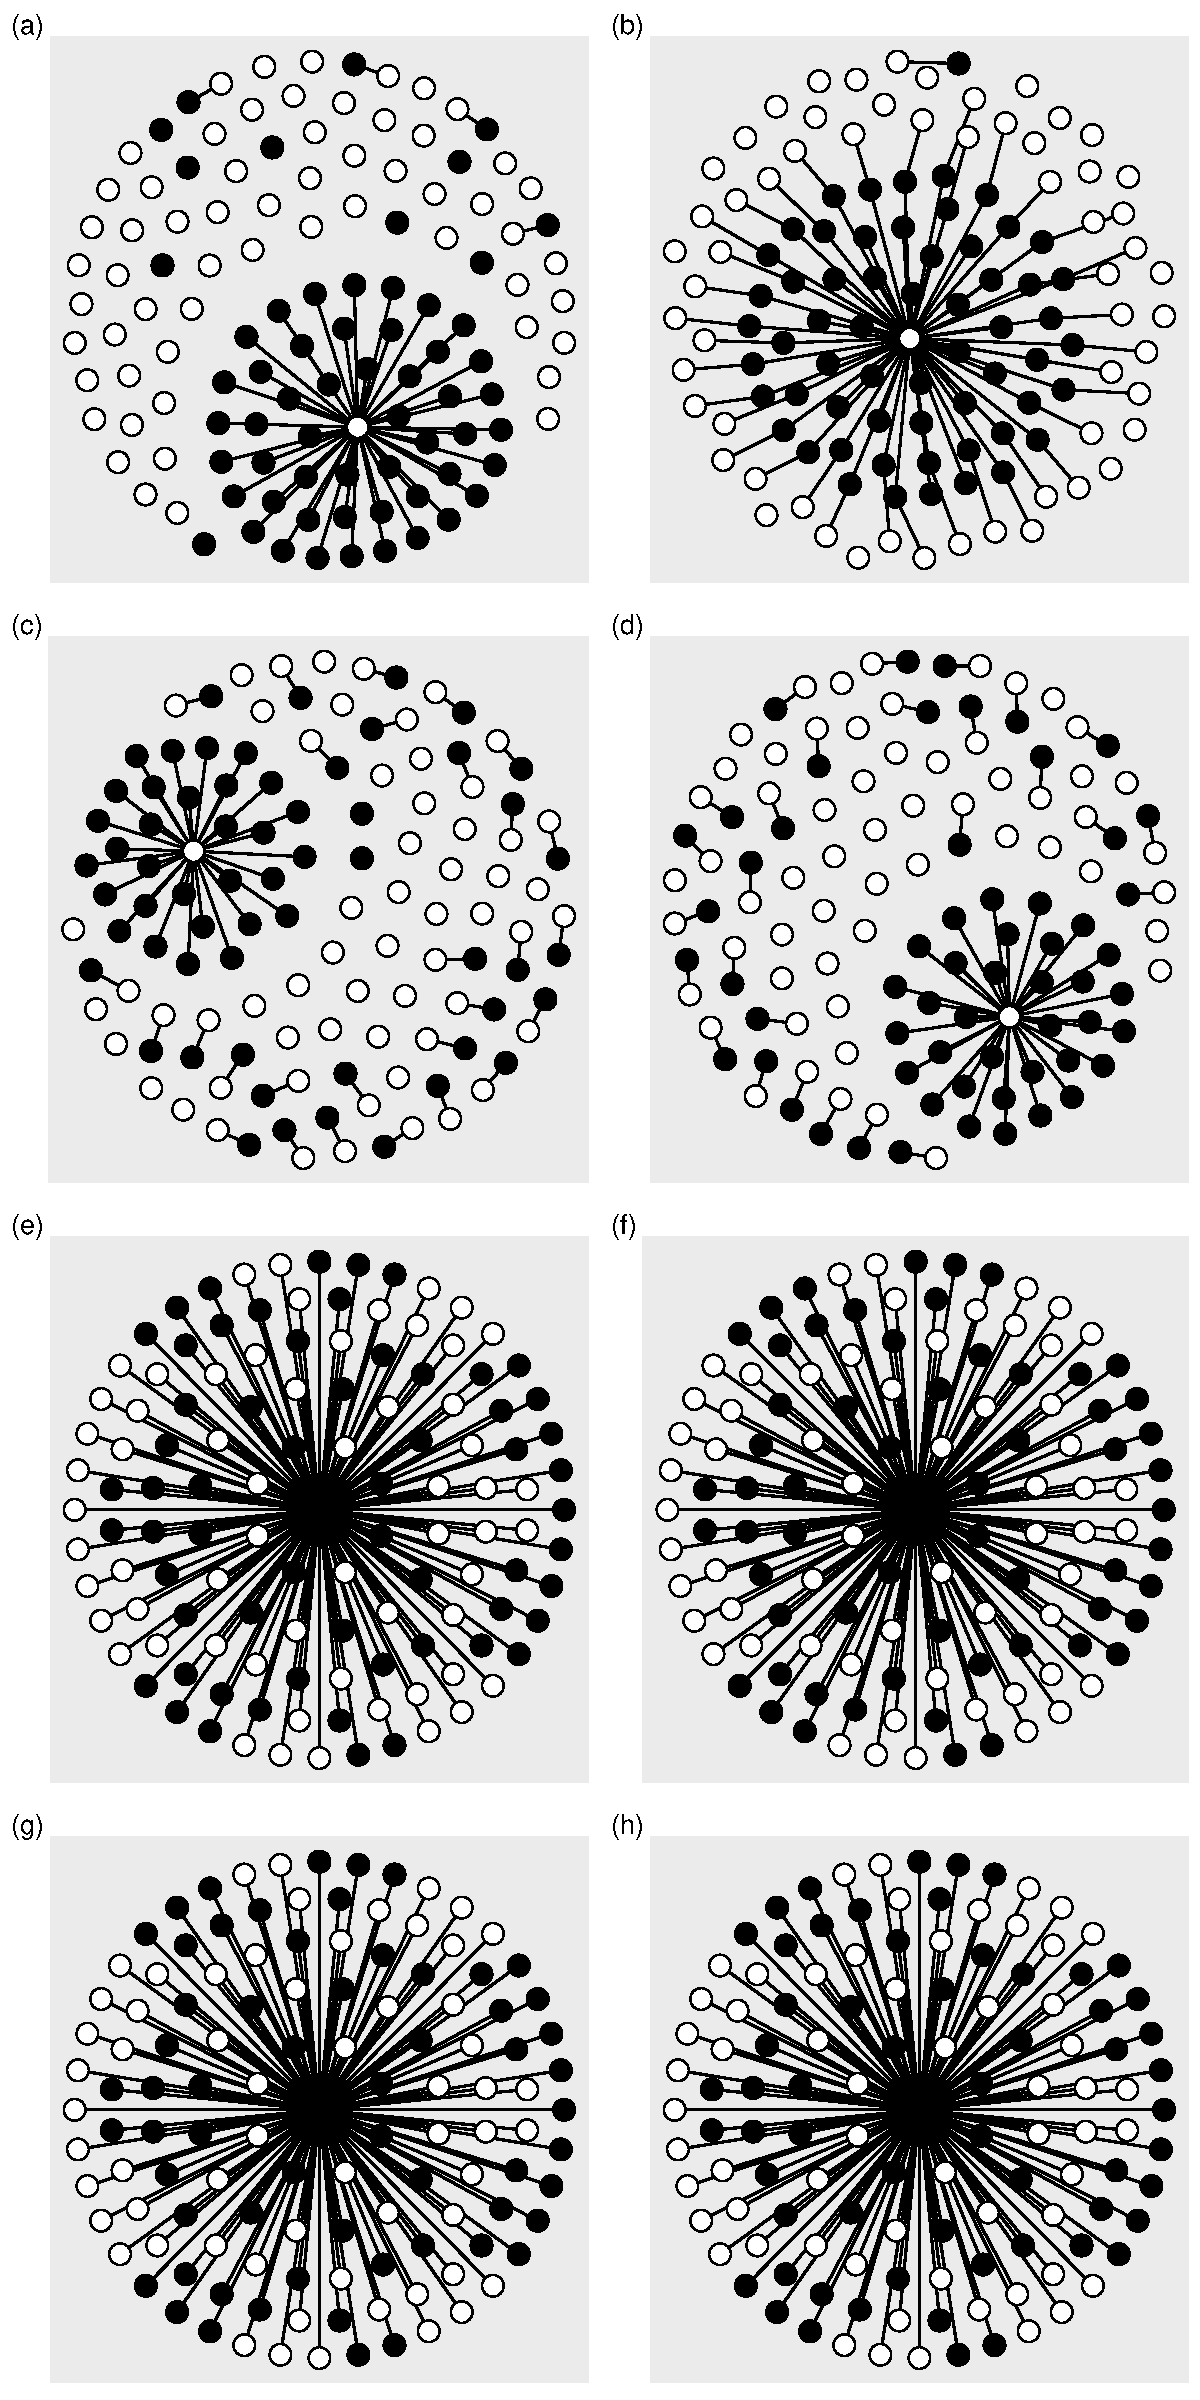
\includegraphics[height=\textheight,width=\textwidth,keepaspectratio]{graphVisualization_firstModel_phi1_nm60_static_oneToOne_allowUnlinked}
  \caption{a}
  \label{fig:graphVisualization_firstModel_phi1_nm60_static_oneToOne_allowUnlinked}
\end{figure}

\begin{figure}
  \centering
  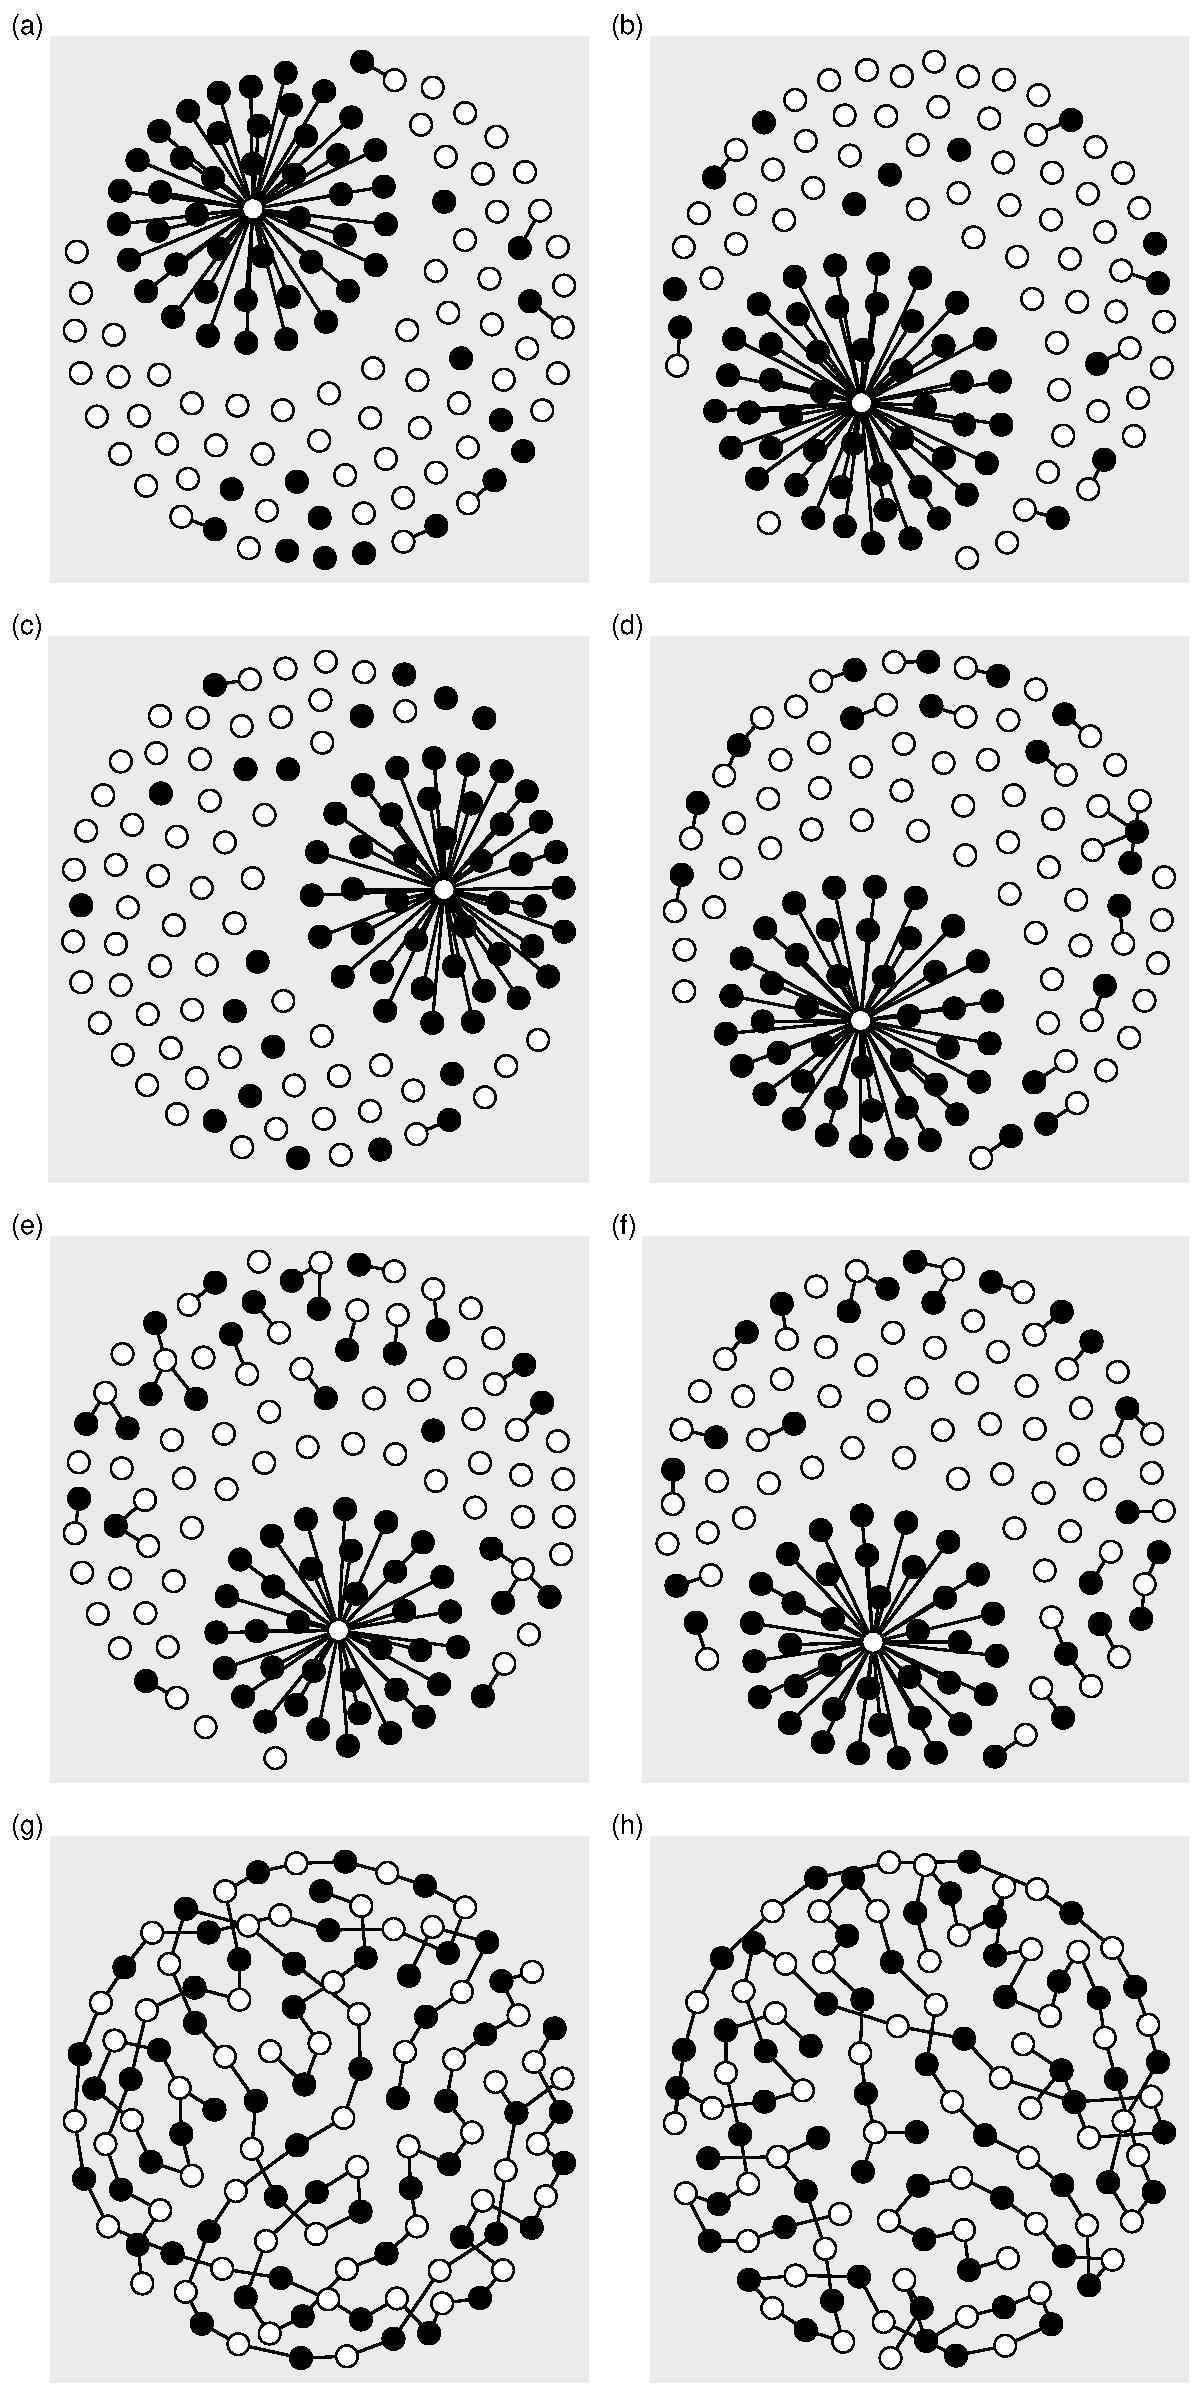
\includegraphics[height=\textheight,width=\textwidth,keepaspectratio]{graphVisualization_firstModel_phi1_nm60_static_complete_allowUnlinked}
  \caption{a}
  \label{fig:graphVisualization_firstModel_phi1_nm60_static_complete_allowUnlinked}
\end{figure}

\begin{figure}
  \centering
  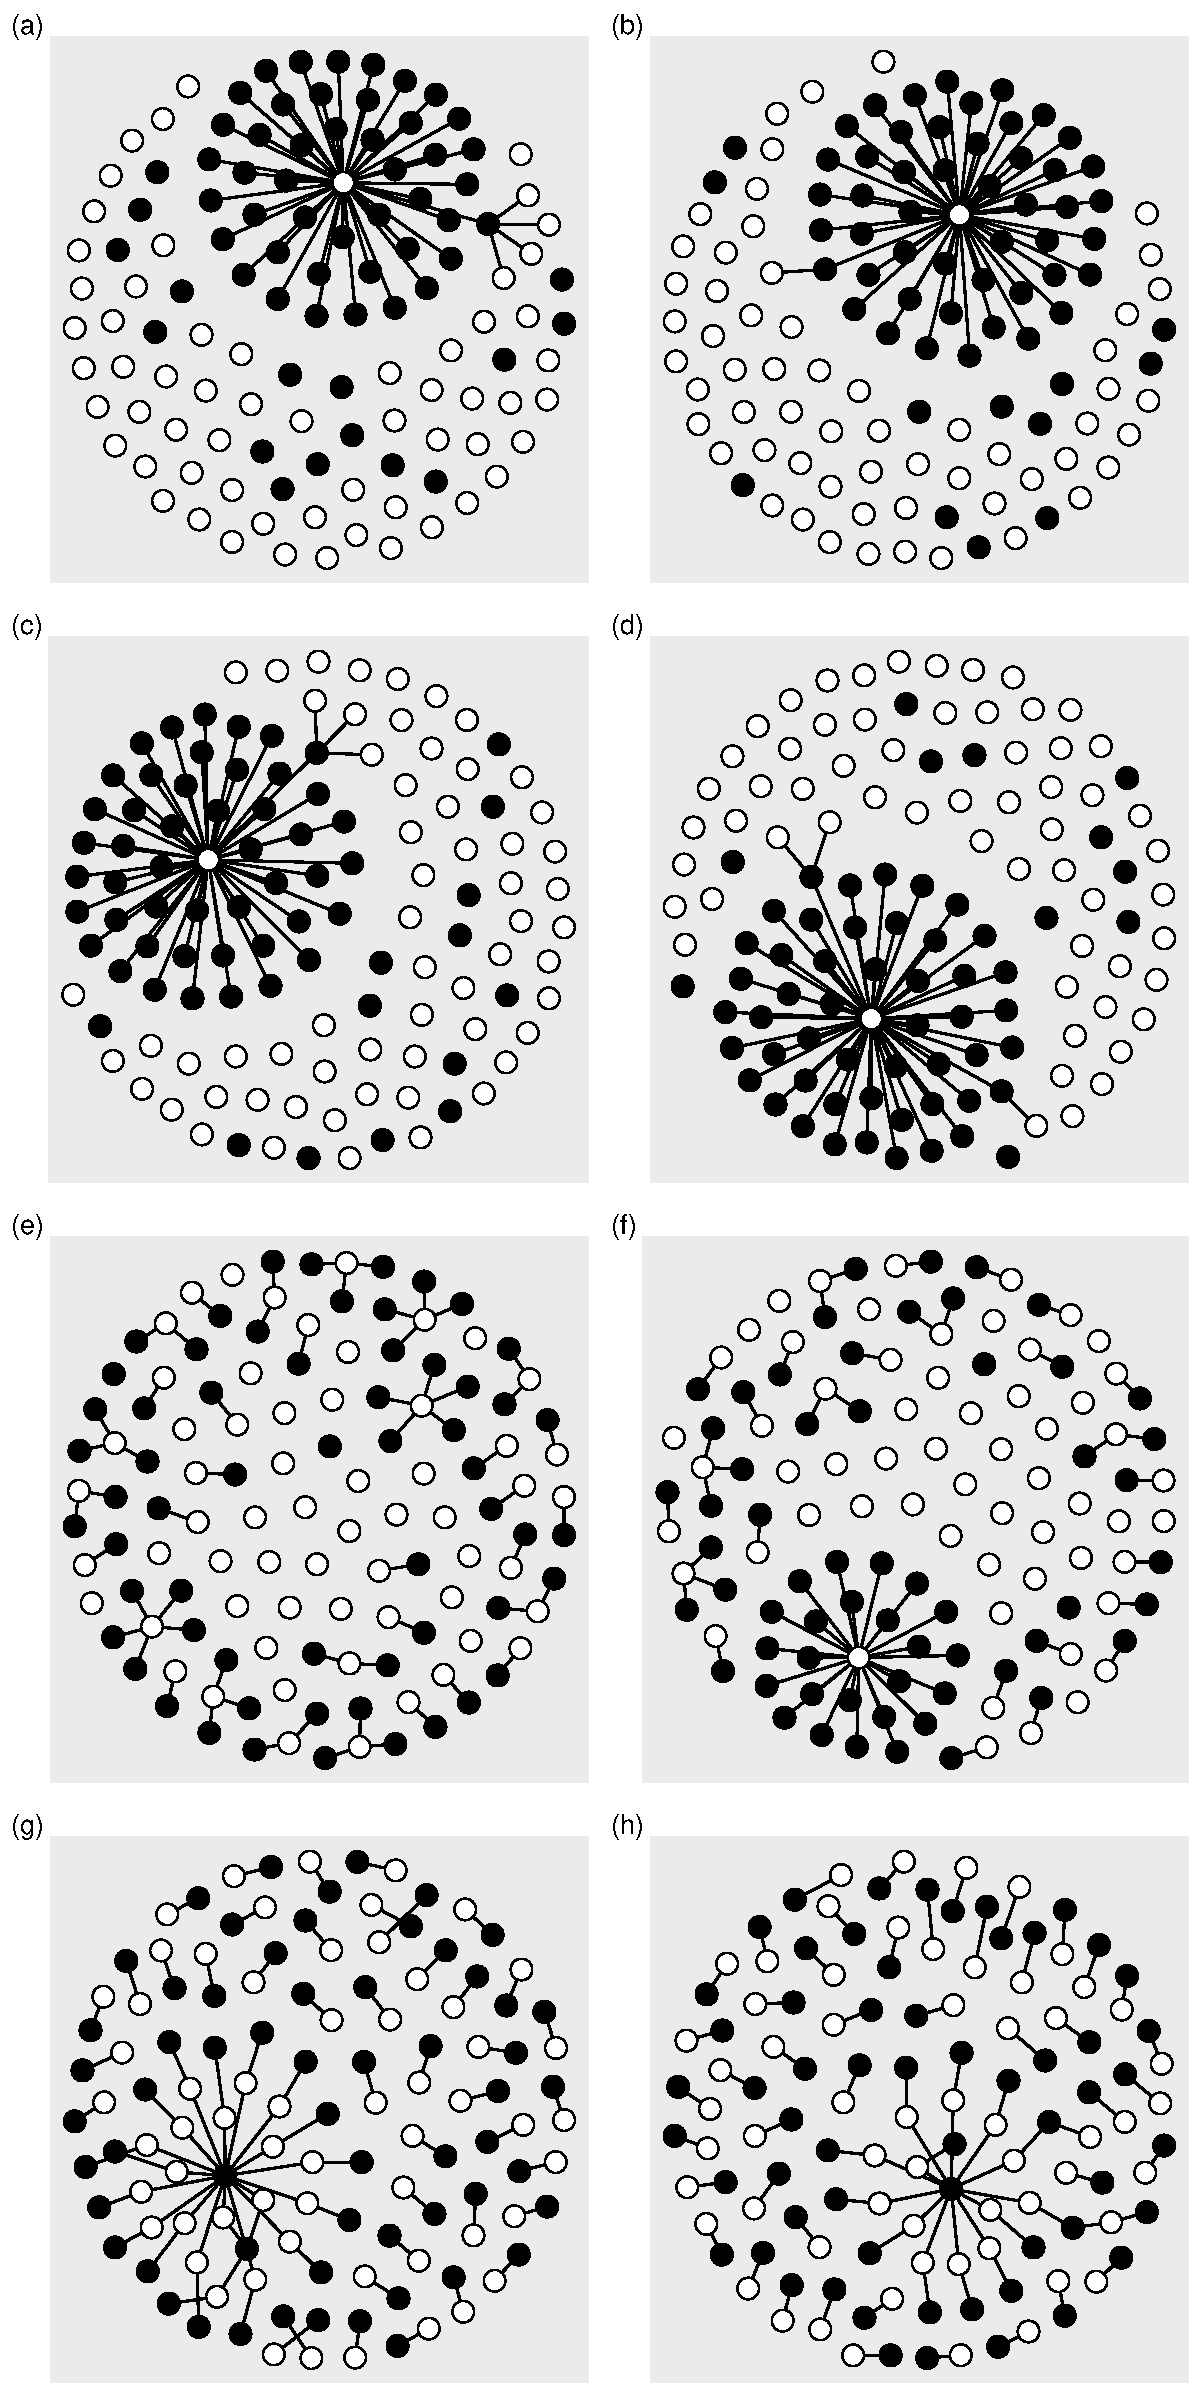
\includegraphics[height=\textheight,width=\textwidth,keepaspectratio]{graphVisualization_uniform_phi1_nm60_static_randomBipartite_allowUnlinked}
  \caption{a}
  \label{fig:graphVisualization_uniform_phi1_nm60_static_randomBipartite_allowUnlinked}
\end{figure}

\begin{figure}
  \centering
  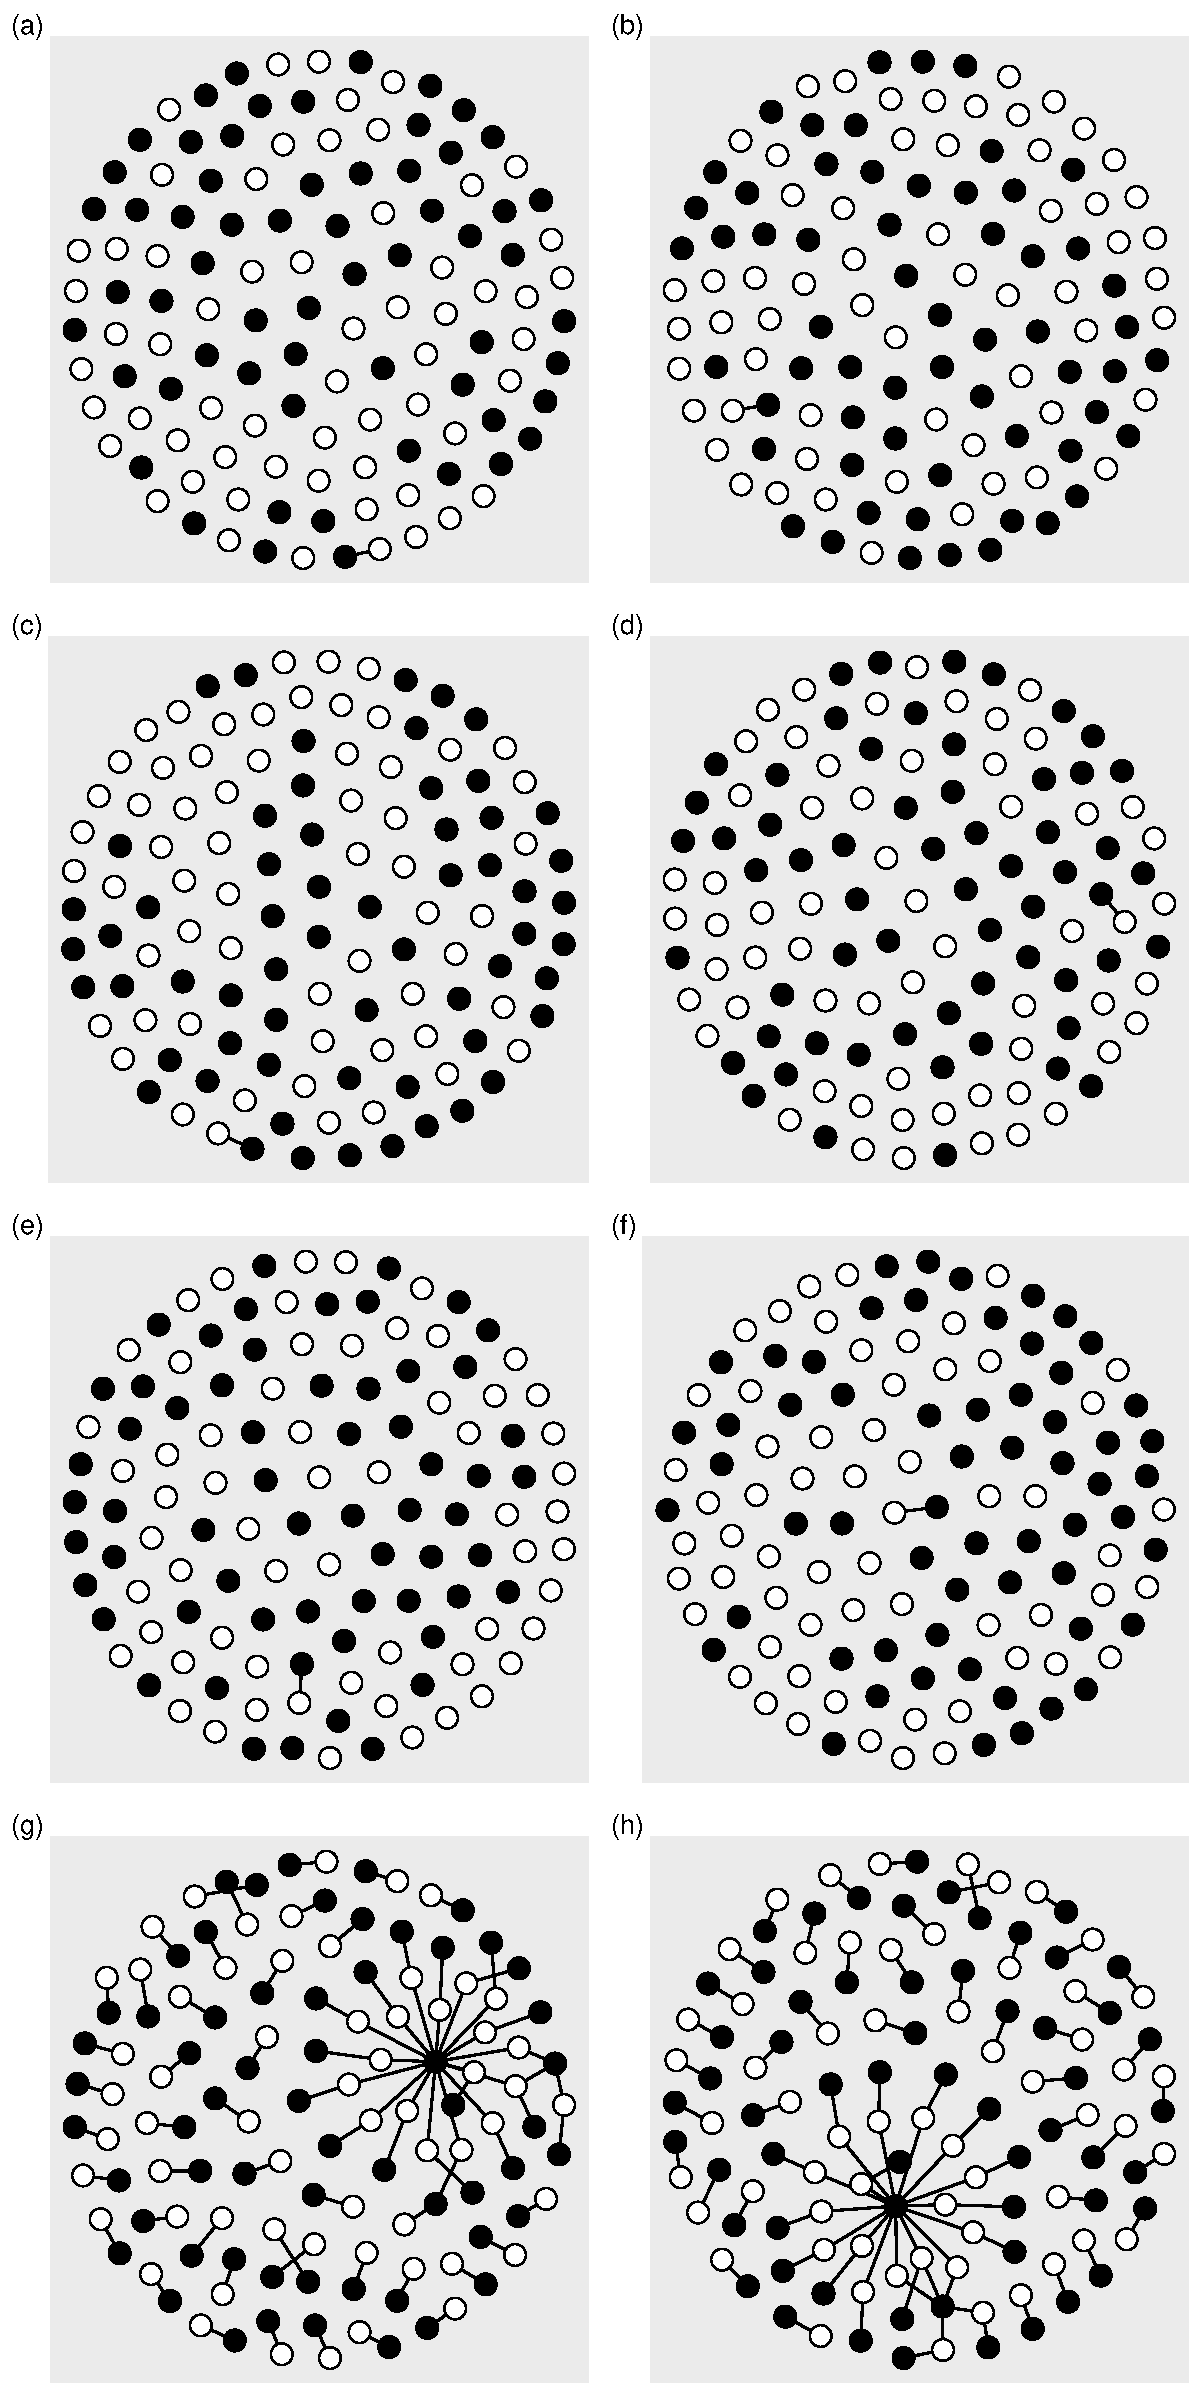
\includegraphics[height=\textheight,width=\textwidth,keepaspectratio]{graphVisualization_uniform_phi1_nm60_static_singleLink_allowUnlinked}
  \caption{a}
  \label{fig:graphVisualization_uniform_phi1_nm60_static_singleLink_allowUnlinked}
\end{figure}

\begin{figure}
  \centering
  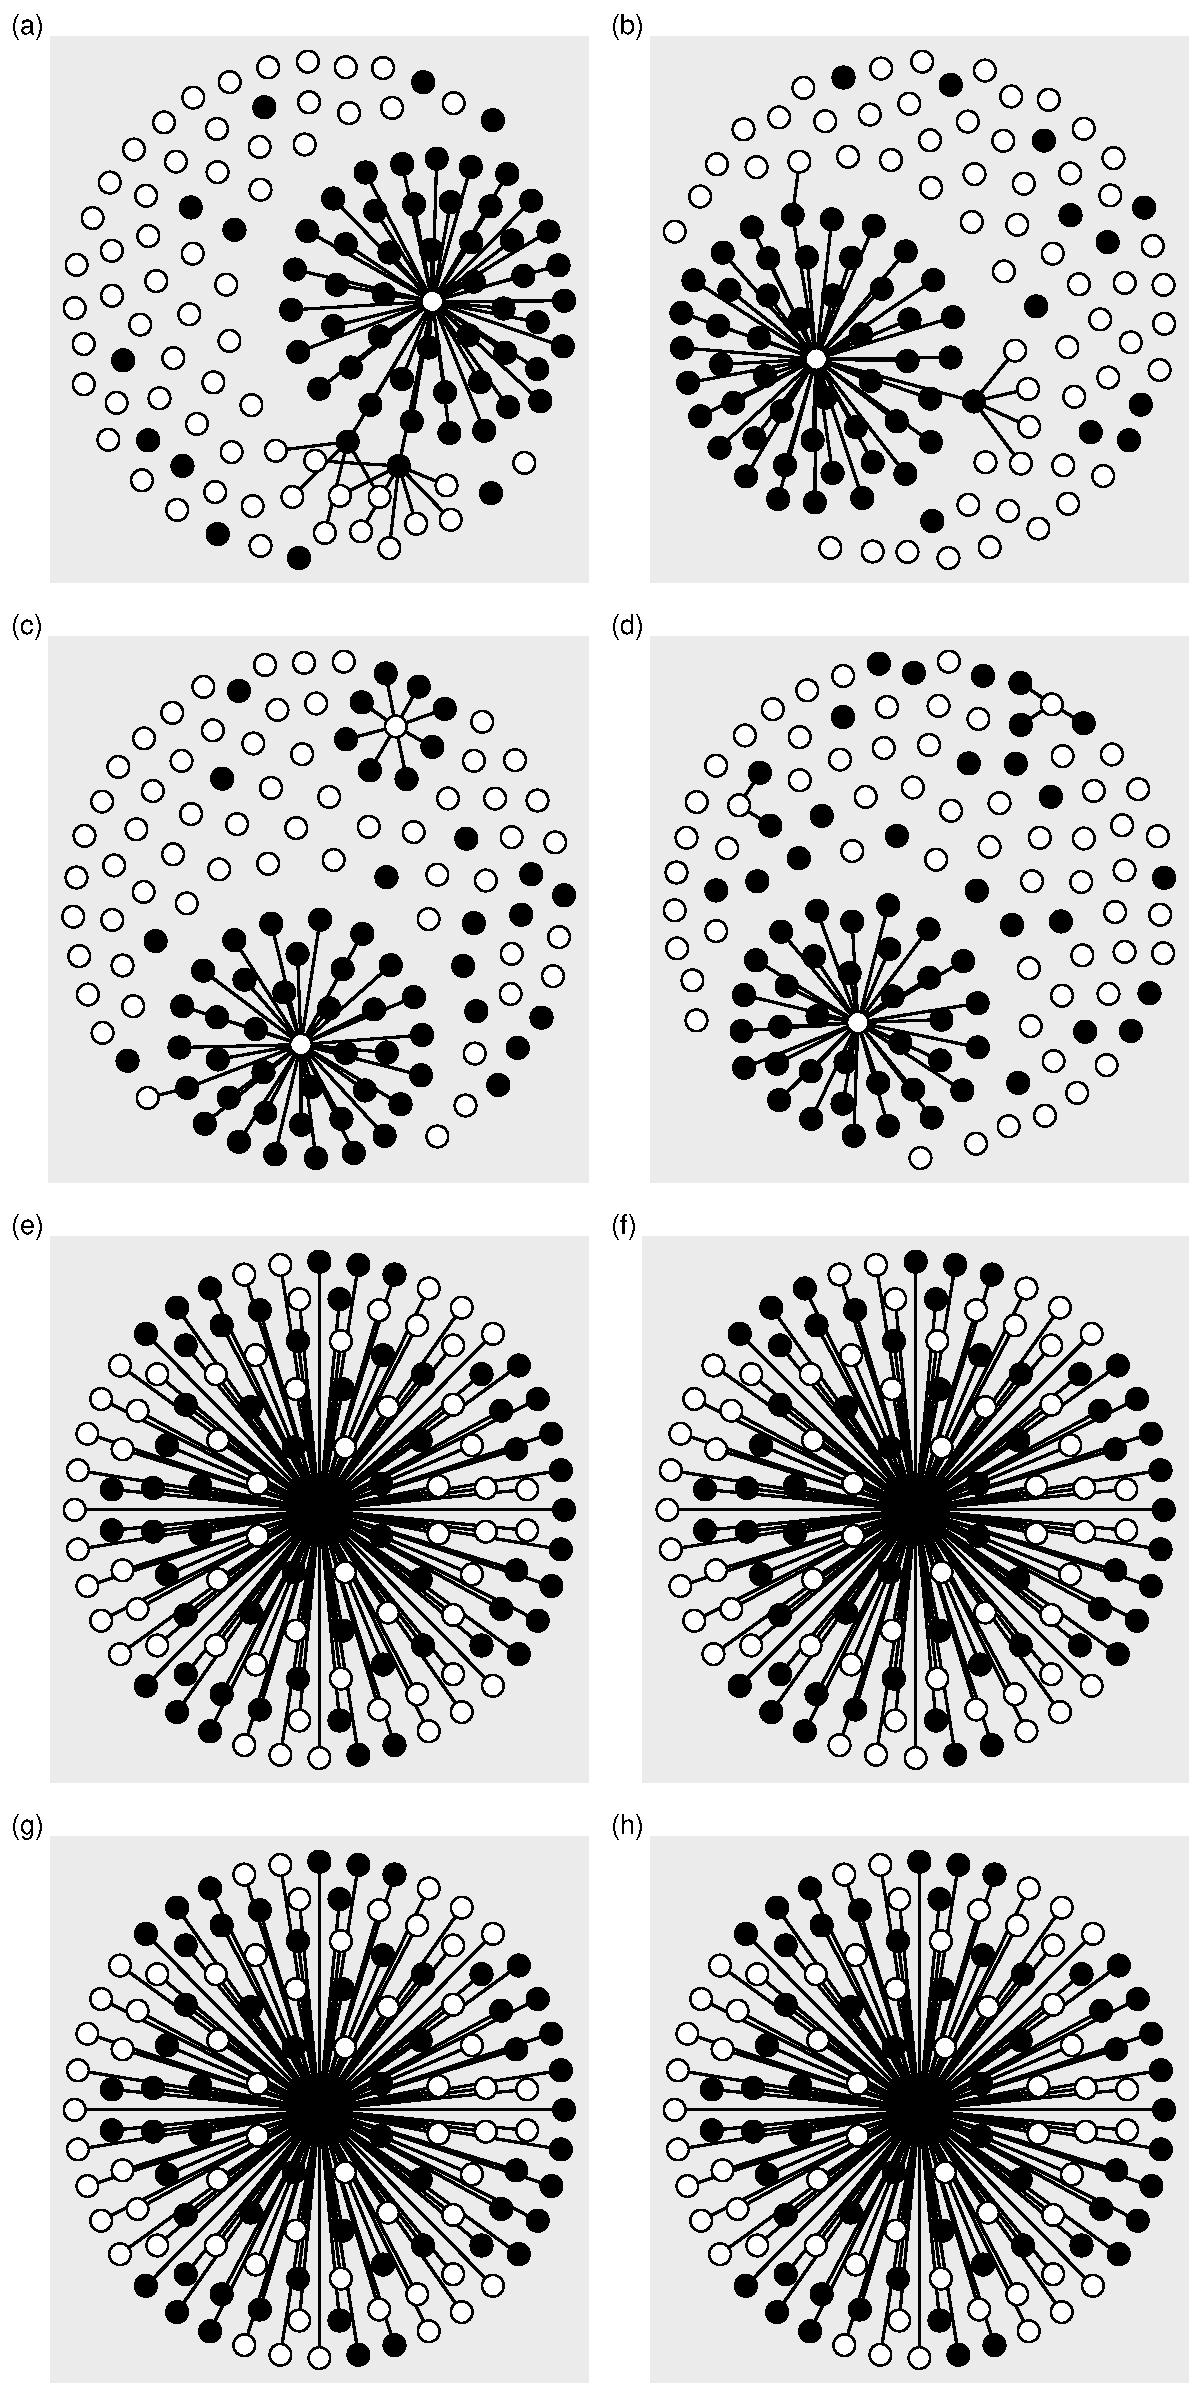
\includegraphics[height=\textheight,width=\textwidth,keepaspectratio]{graphVisualization_uniform_phi1_nm60_static_oneToOne_allowUnlinked}
  \caption{a}
  \label{fig:graphVisualization_uniform_phi1_nm60_static_oneToOne_allowUnlinked}
\end{figure}

\begin{figure}
  \centering
  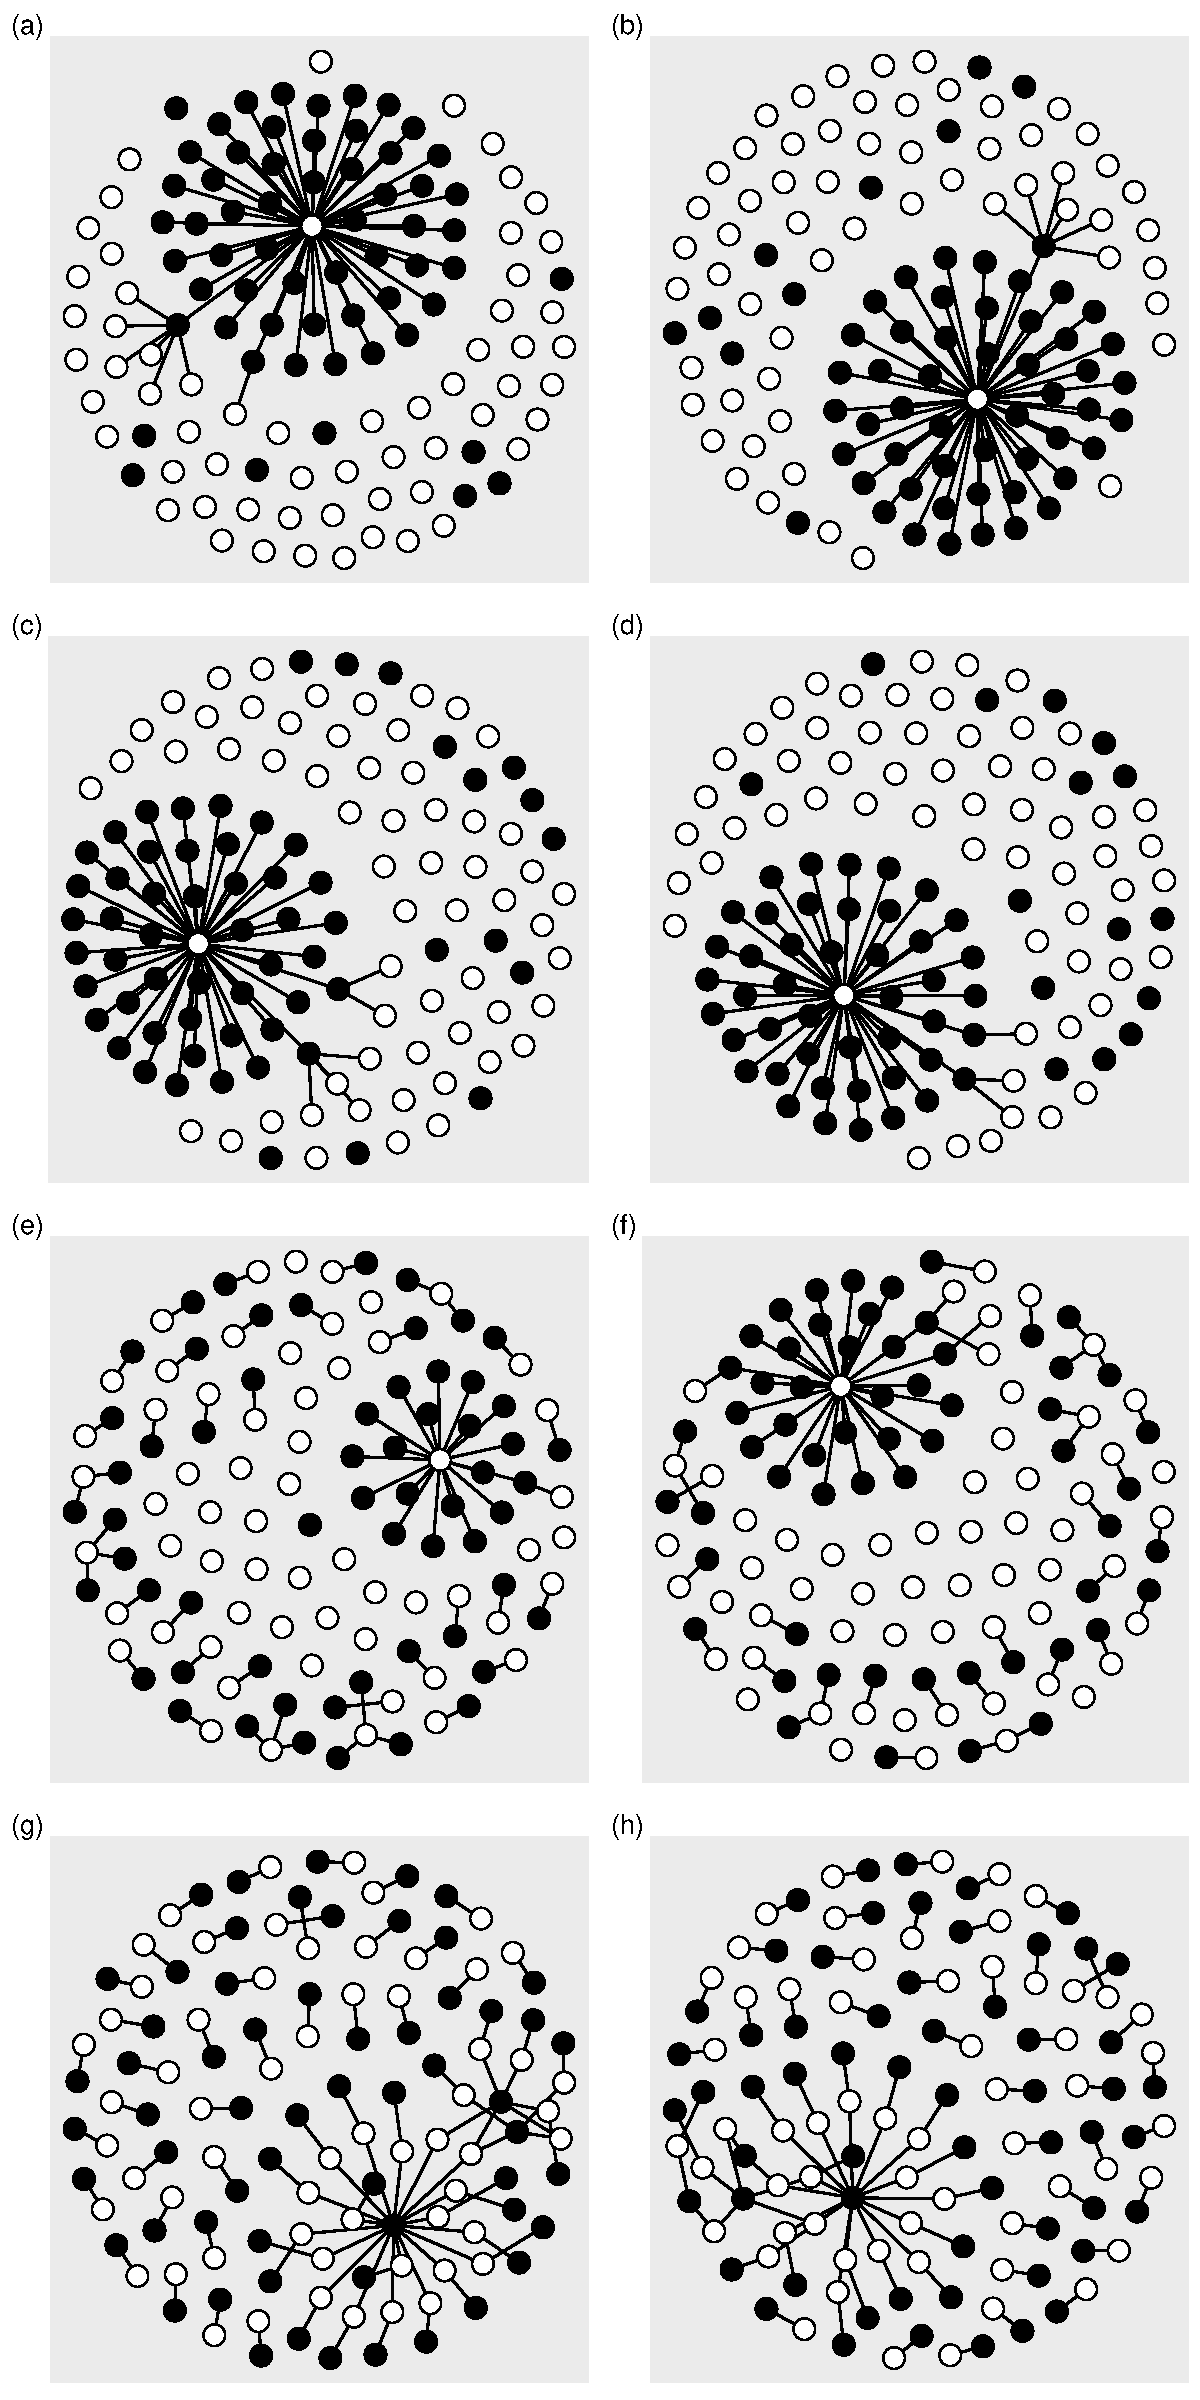
\includegraphics[height=\textheight,width=\textwidth,keepaspectratio]{graphVisualization_uniform_phi1_nm60_static_complete_allowUnlinked}
  \caption{a}
  \label{fig:graphVisualization_uniform_phi1_nm60_static_complete_allowUnlinked}
\end{figure}


\subsection{Information theoretic and statistical measures}
\label{sec:results_new_other}

This section shows the data obtained from executing simulations with various sets of parameters.
All simulations are run with a graph size of $n=m=400$.
Every experiment in this section is the result of averaging at least 20 realizations.
Most experiments consist of 100 realizations.
Some had to be reduced to 20 realizations due to the total running time and are marked as such.
Results for $\phi=0$ and $\phi=1$ are shown.
Three different initial conditions are tested: random bipartite graph, single link and one-to-one.
For the \secondmodel{} only results for $\pi$ following a uniform probability distribution are shown.
The chosen $\lambda$ value for which curves are fitted is the one that's qualitatively closer to a power law.

For the \firstmodel{} with $\phi=0$, Figures \ref{fig:informationTheoretic_firstModel_phi0_nm400_dynamic_randomBipartite_allowUnlinked}, \ref{fig:informationTheoretic_firstModel_phi0_nm400_dynamic_singleLink_allowUnlinked} and \ref{fig:informationTheoretic_firstModel_phi0_nm400_dynamic_oneToOne_allowUnlinked} show the information theoretic measures of the optimal graph for values of $\lambda$ ranging from 0 to 1.
They correspond to the random graph, single link and one-to-one initial graphs respectively.

\begin{figure}
  \centering
  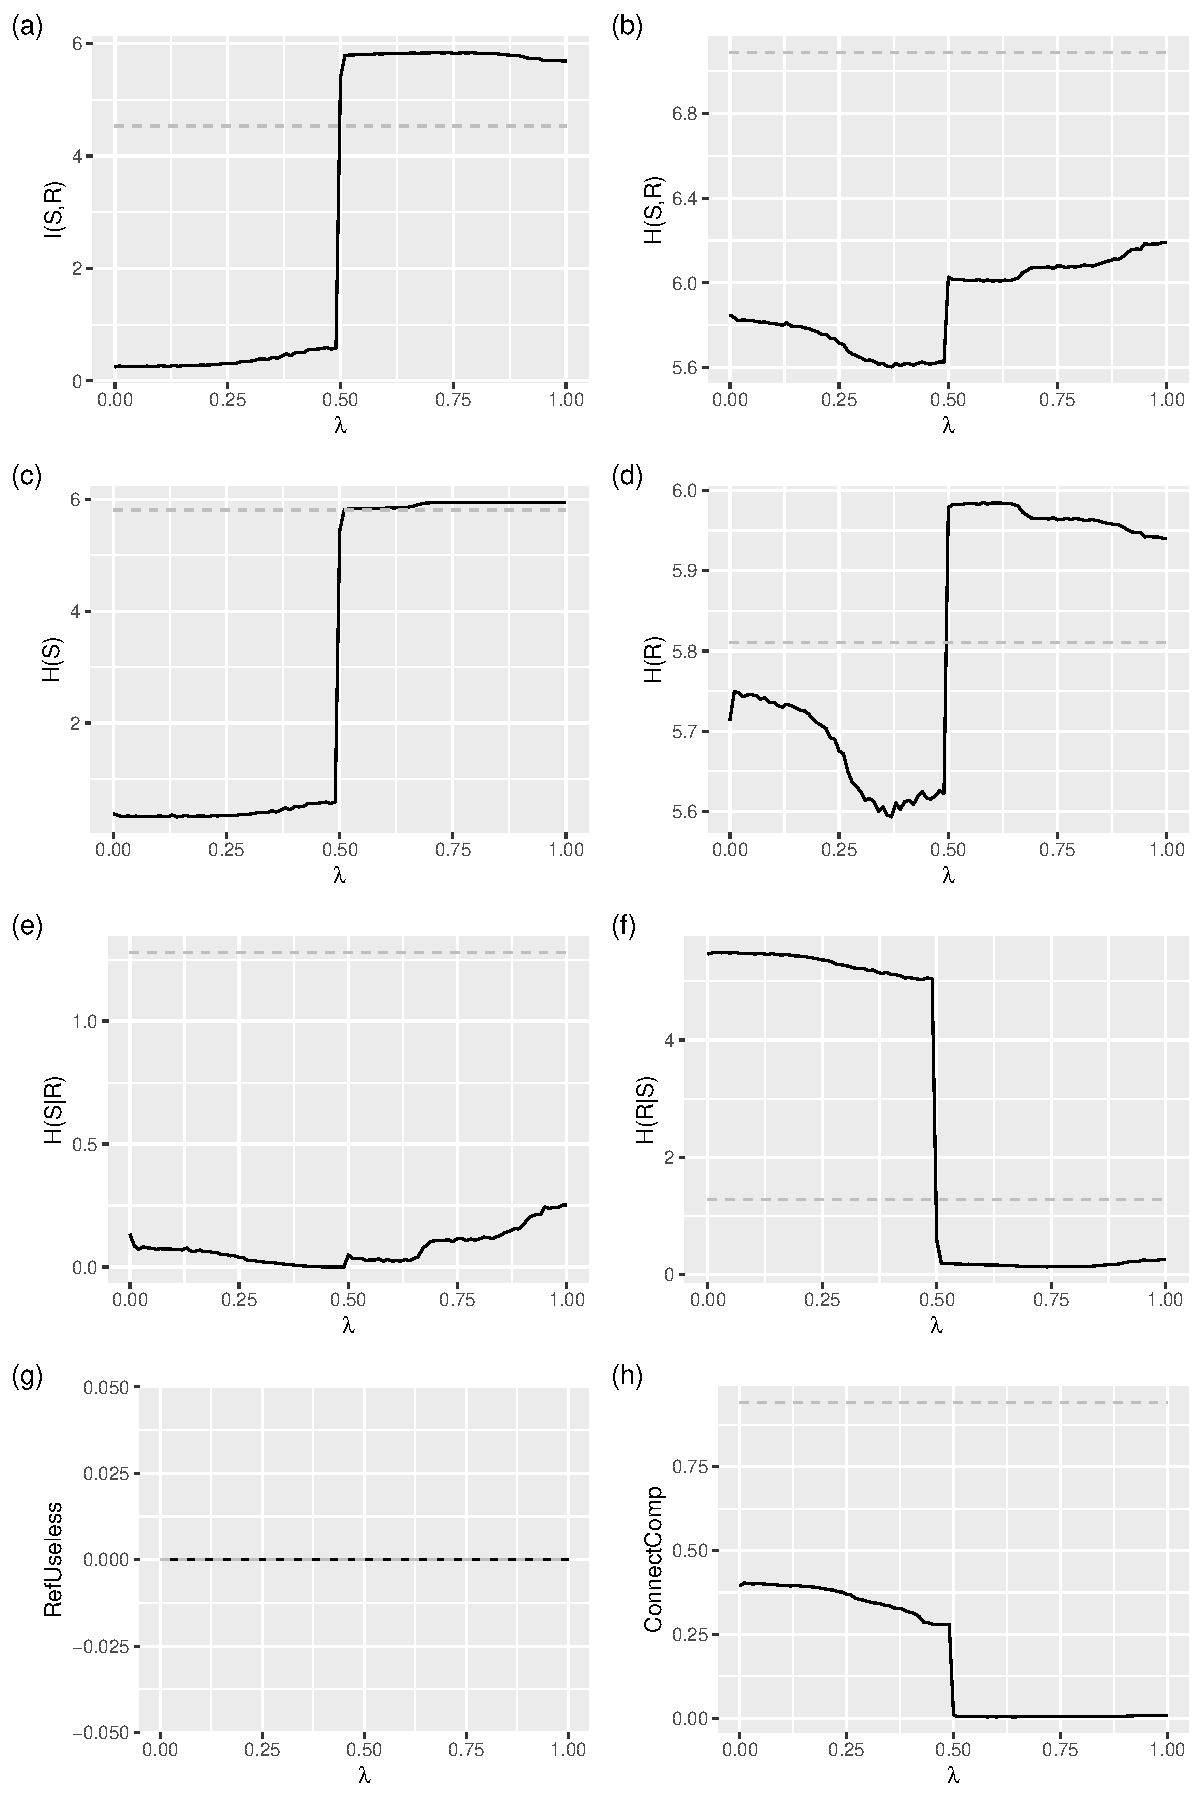
\includegraphics[width=\textwidth]{informationTheoretic_firstModel_phi0_nm400_dynamic_randomBipartite_allowUnlinked}
  \caption{a}
  \label{fig:informationTheoretic_firstModel_phi0_nm400_dynamic_randomBipartite_allowUnlinked}
\end{figure}

\begin{figure}
  \centering
  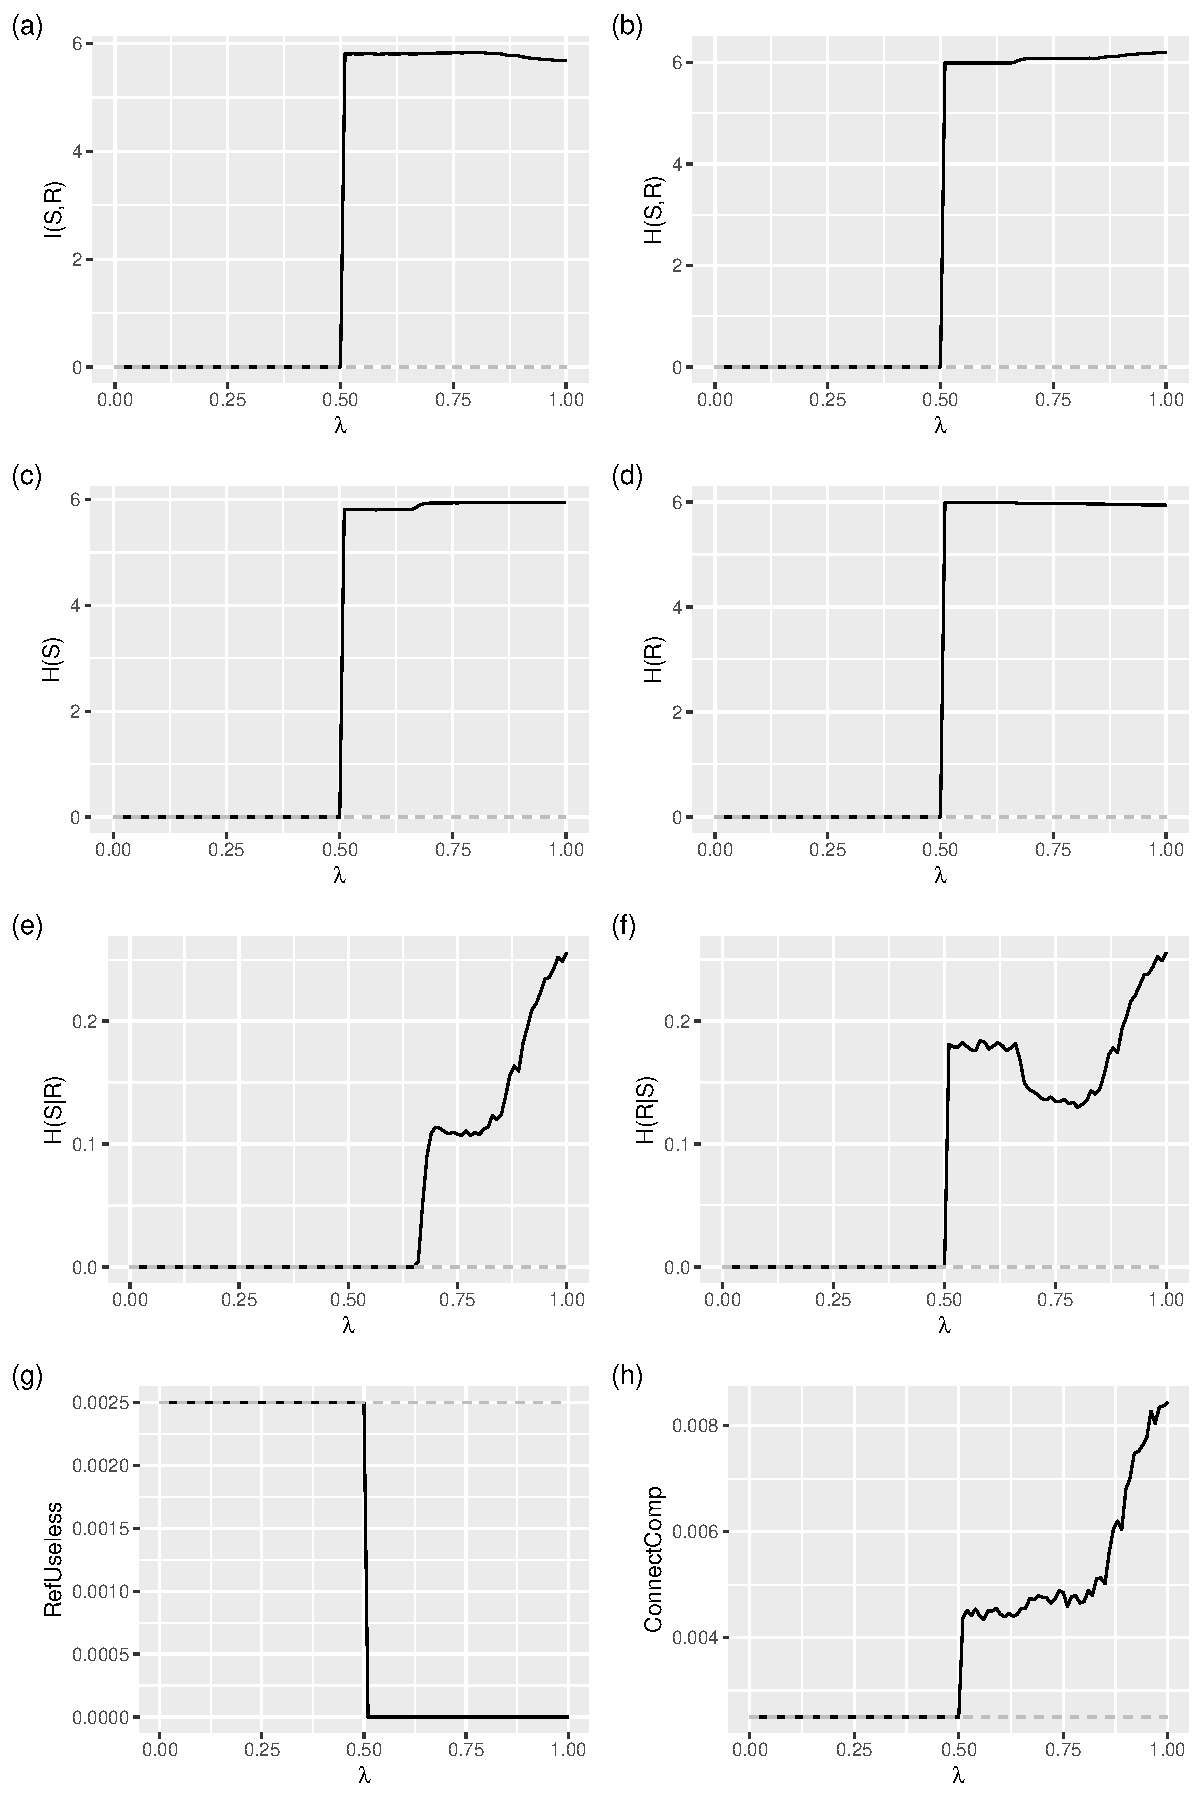
\includegraphics[width=\textwidth]{informationTheoretic_firstModel_phi0_nm400_dynamic_singleLink_allowUnlinked}
  \caption{a}
  \label{fig:informationTheoretic_firstModel_phi0_nm400_dynamic_singleLink_allowUnlinked}
\end{figure}

\begin{figure}
  \centering
  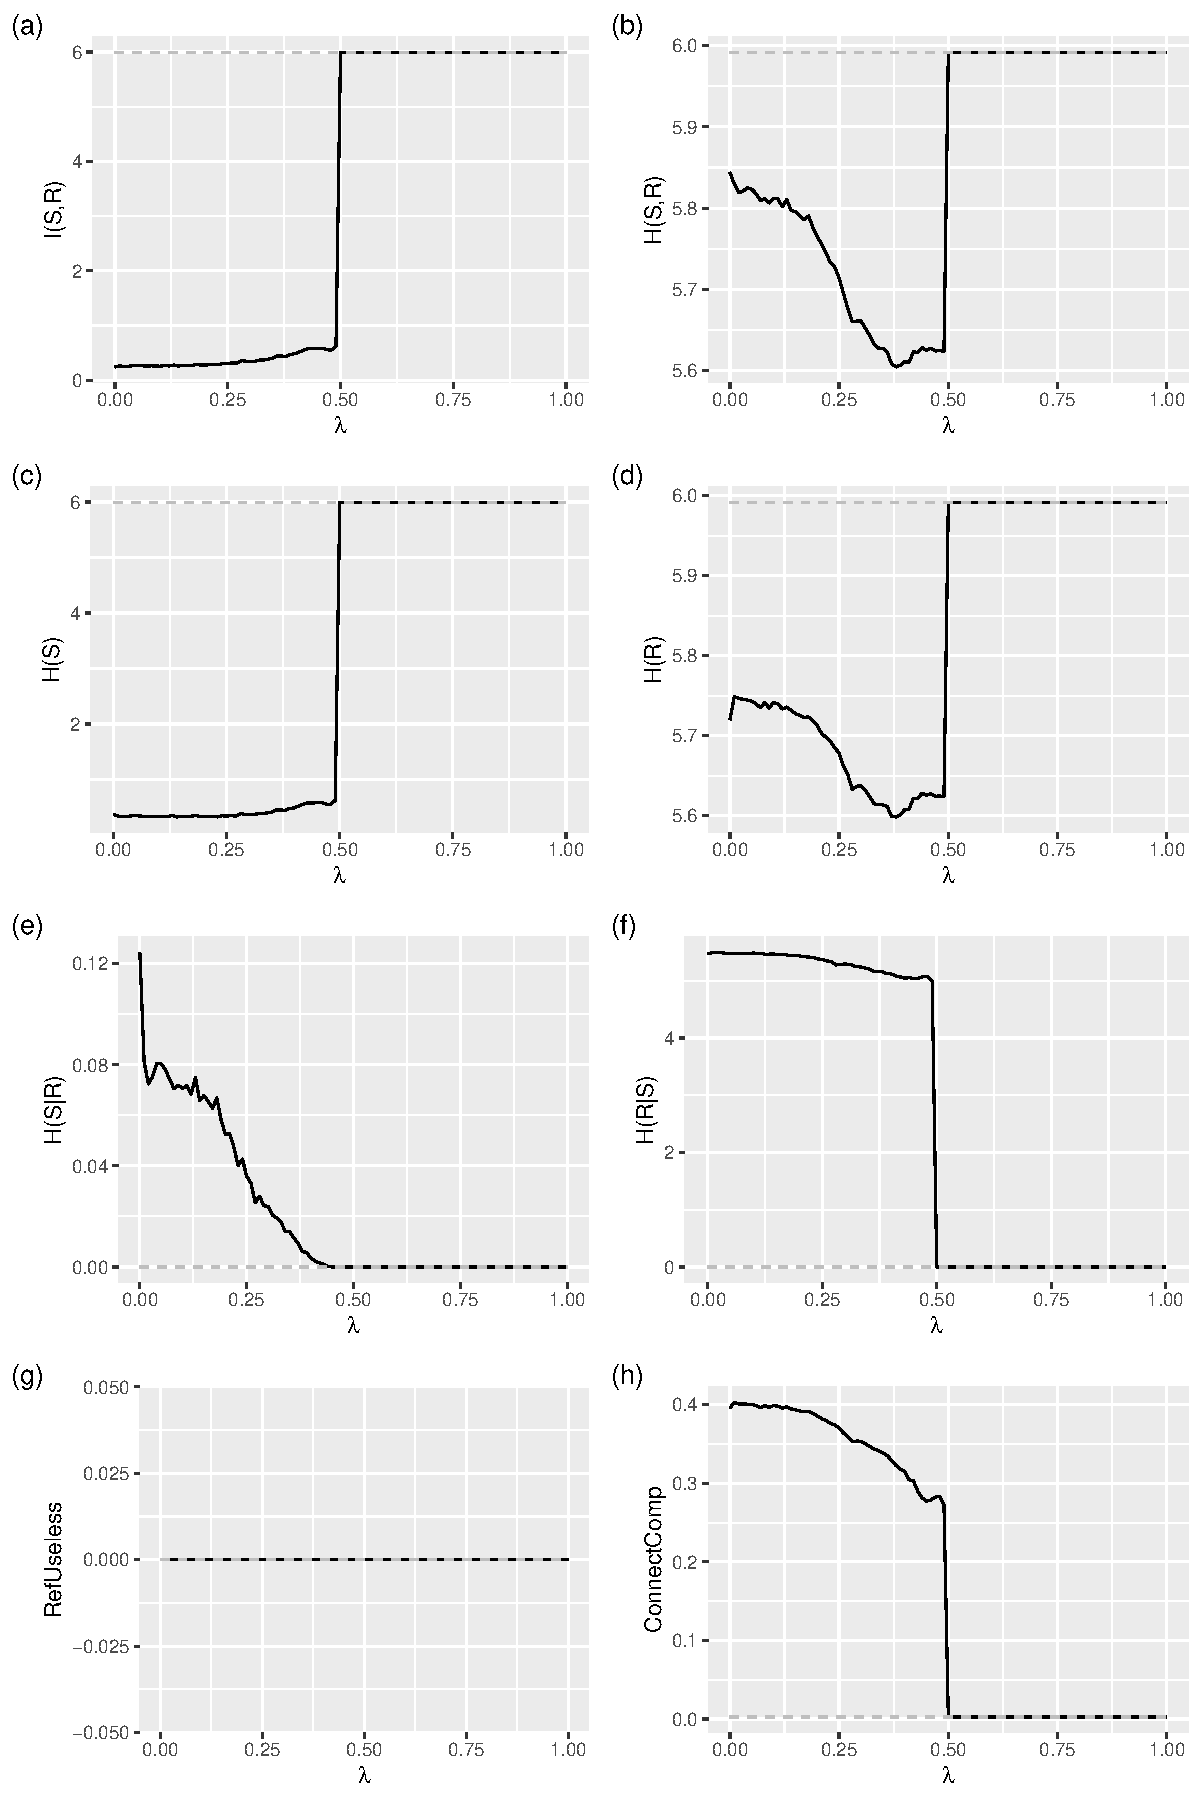
\includegraphics[width=\textwidth]{informationTheoretic_firstModel_phi0_nm400_dynamic_oneToOne_allowUnlinked}
  \caption{a}
  \label{fig:informationTheoretic_firstModel_phi0_nm400_dynamic_oneToOne_allowUnlinked}
\end{figure}

Figures \ref{fig:insideLambda_firstModel_phi0_nm400_dynamic_randomBipartite_allowUnlinked} and \ref{fig:insideLambda_firstModel_phi0_nm400_dynamic_oneToOne_allowUnlinked} (random and one-to-one initial conditions respectively) show statistical measures of select values of $\lambda$, with Figures \ref{fig:fitting_insideLambda_firstModel_phi0_nm400_dynamic_randomBipartite_allowUnlinked} and \ref{fig:fitting_insideLambda_firstModel_phi0_nm400_dynamic_oneToOne_allowUnlinked} (random and one-to-one respectively) showing the fitting of the curve to a power law for a single select value of $\lambda$ and Tables \ref{tab:fitting_insideLambda_firstModel_phi0_nm400_dynamic_randomBipartite_allowUnlinked} and \ref{tab:fitting_insideLambda_firstModel_phi0_nm400_dynamic_oneToOne_allowUnlinked} (random and one-to-one respectively) showing the values of the regression exponent and factor.
The single link initial condition is not plotted for select values of $\lambda$ as it fails to evolve beyond the single link state.

\begin{figure}
  \centering
  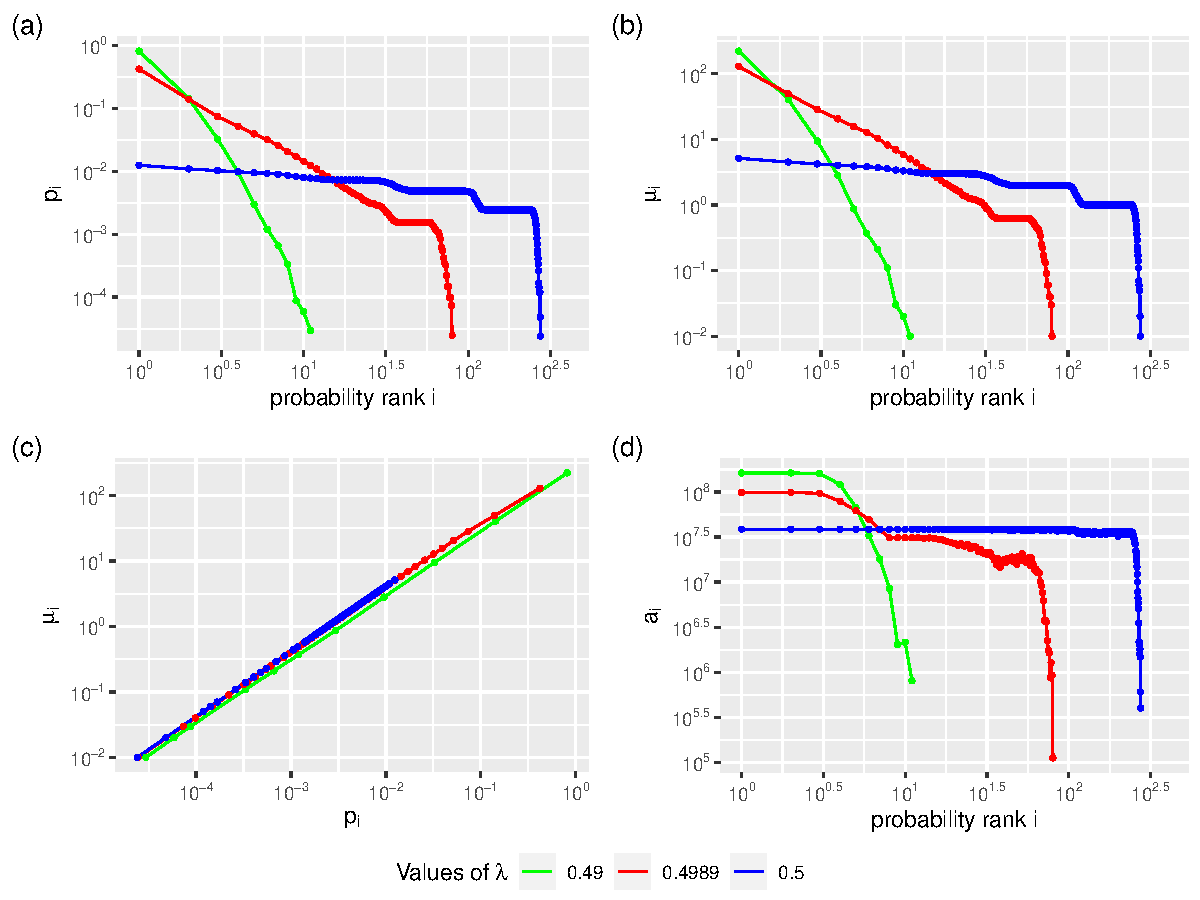
\includegraphics[width=\textwidth]{insideLambda_firstModel_phi0_nm400_dynamic_randomBipartite_allowUnlinked}
  \caption{0.4989}
  \label{fig:insideLambda_firstModel_phi0_nm400_dynamic_randomBipartite_allowUnlinked}
\end{figure}

\begin{figure}
  \centering
  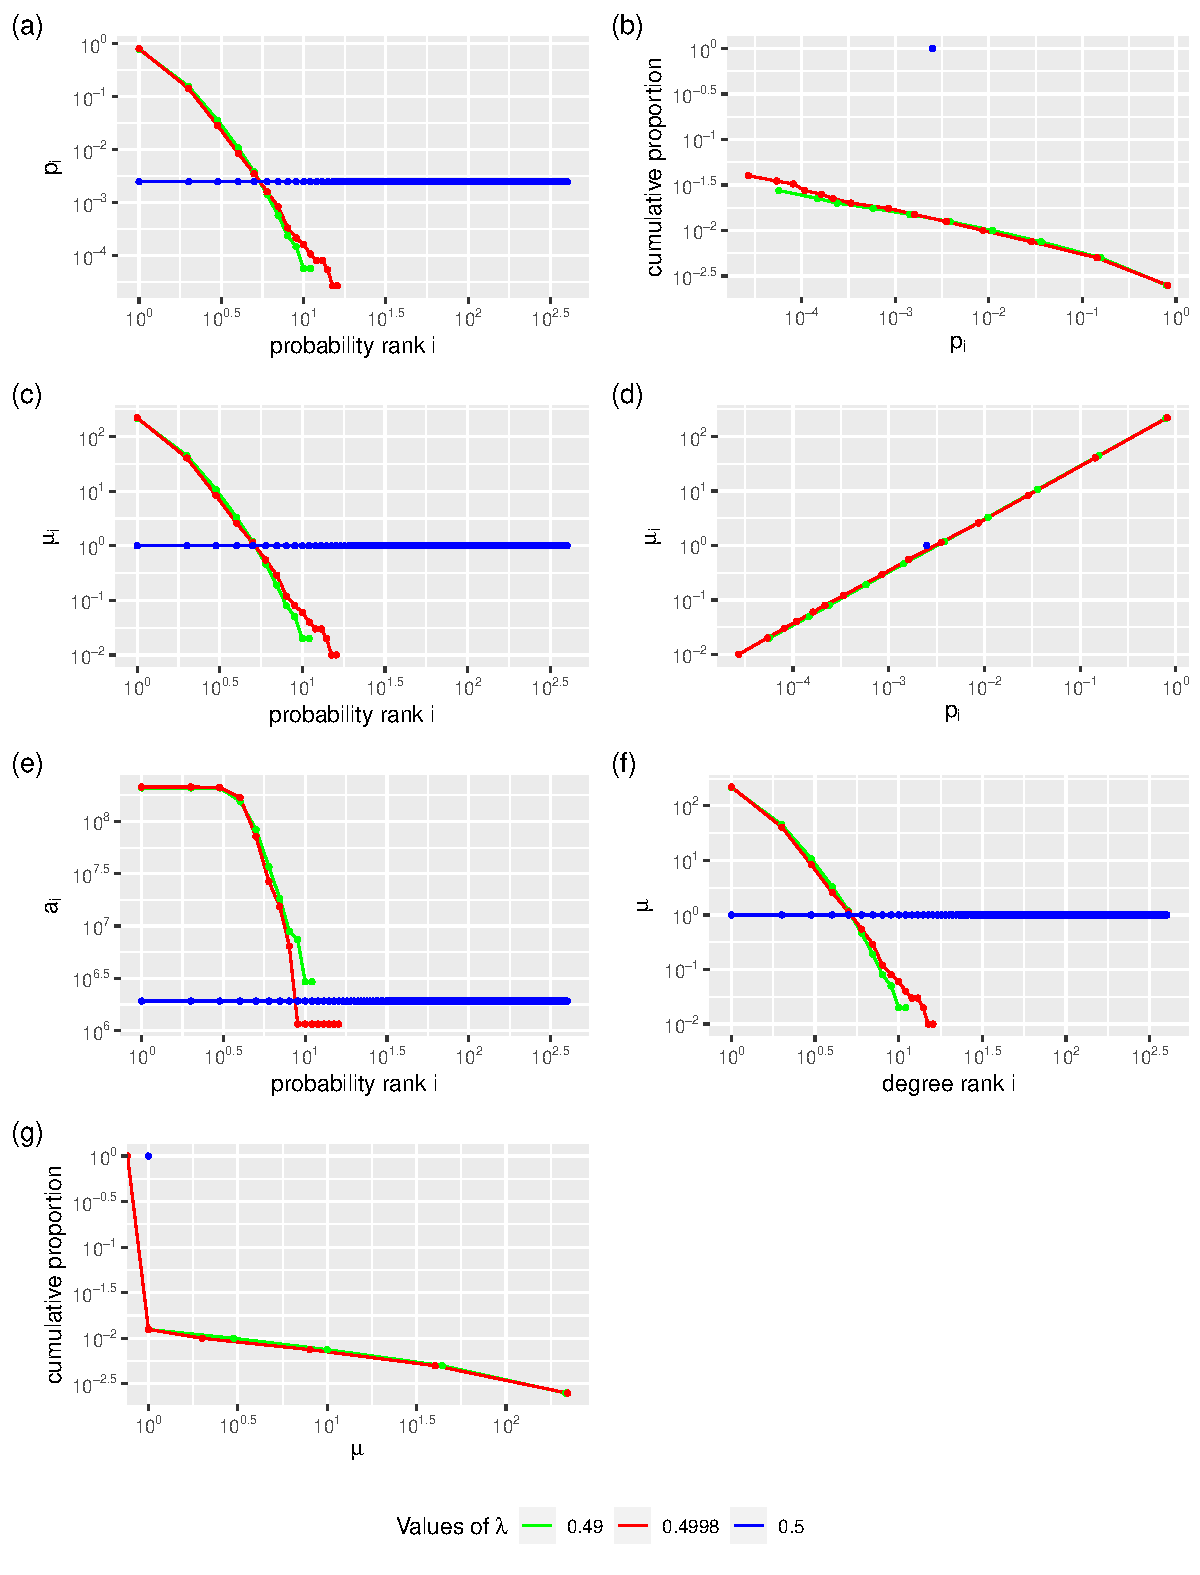
\includegraphics[width=\textwidth]{insideLambda_firstModel_phi0_nm400_dynamic_oneToOne_allowUnlinked}
  \caption{0.998}
  \label{fig:insideLambda_firstModel_phi0_nm400_dynamic_oneToOne_allowUnlinked}
\end{figure}

\begin{figure}
  \centering
  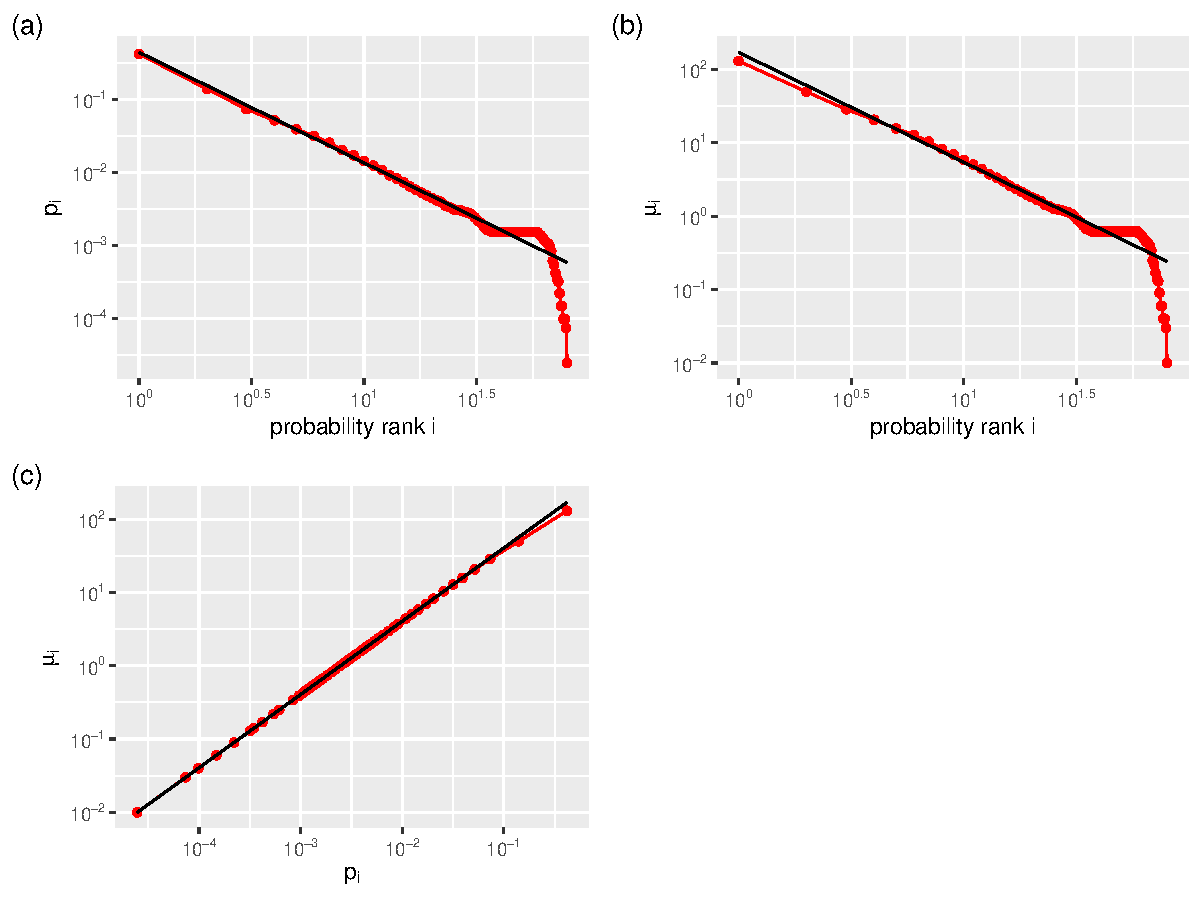
\includegraphics[width=\textwidth]{fitting_insideLambda_firstModel_phi0_nm400_dynamic_randomBipartite_allowUnlinked}
  \caption{0.4989}
  \label{fig:fitting_insideLambda_firstModel_phi0_nm400_dynamic_randomBipartite_allowUnlinked}
\end{figure}

\begin{figure}
  \centering
  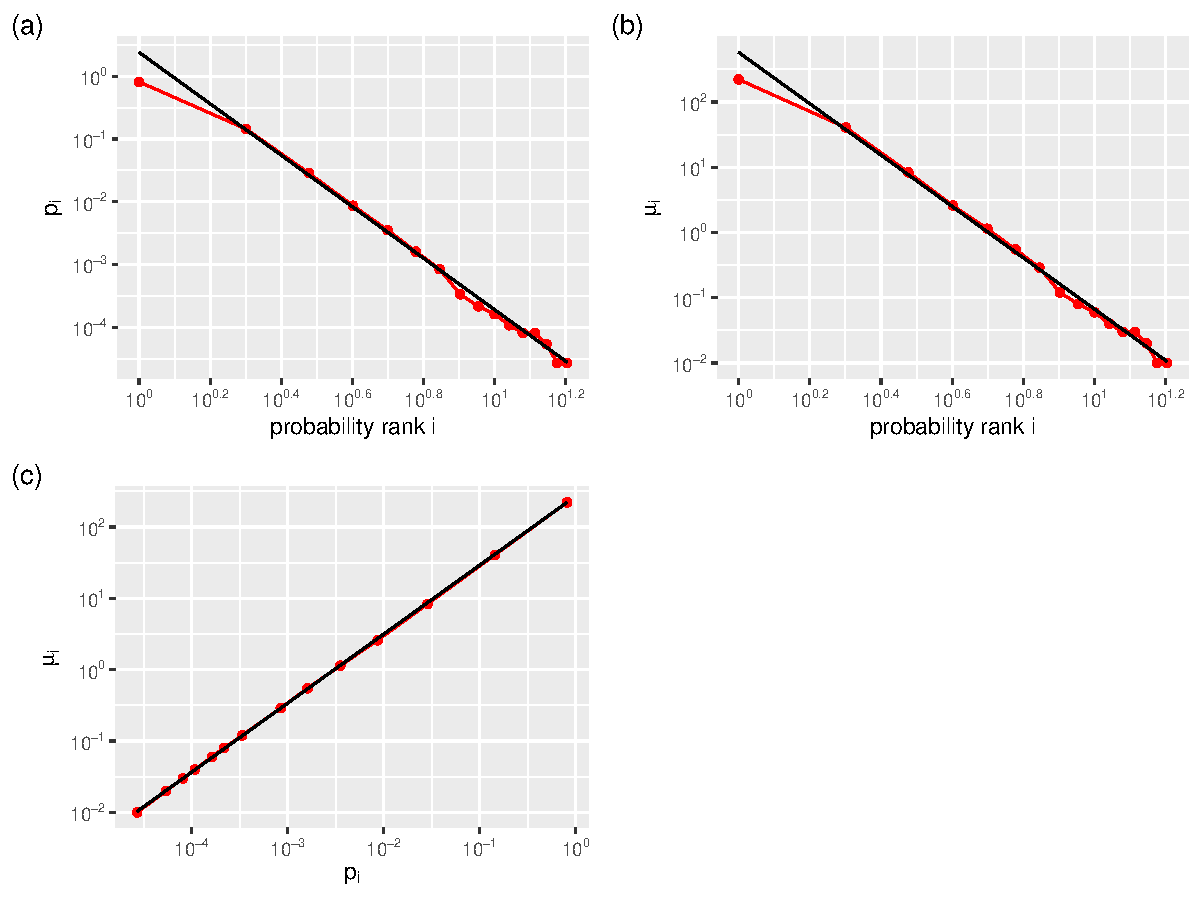
\includegraphics[width=\textwidth]{fitting_insideLambda_firstModel_phi0_nm400_dynamic_oneToOne_allowUnlinked}
  \caption{0.4998}
  \label{fig:fitting_insideLambda_firstModel_phi0_nm400_dynamic_oneToOne_allowUnlinked}
\end{figure}

% latex table generated in R 4.0.4 by xtable 1.8-4 package
% Wed Mar 17 14:20:58 2021
\begin{table}
\centering
\begin{tabular}{lrr}
  \hline
plot & $\alpha$ & $k$ \\ 
  \hline
a & 1.5131590 & 0.4415009 \\ 
  b & 0.6406267 & 0.0016491 \\ 
  c & 1.4972982 & 170.7165580 \\ 
  d & -0.9992804 & 403.8279052 \\ 
  f & 1.4972982 & 170.7165580 \\ 
  g & 0.6725912 & 0.0750000 \\ 
   \hline
\end{tabular}
\caption{
  Table showing the exponent ($\alpha$) and the factor ($k$) of the power laws fitted in Figure \ref{fig:fitting_insideLambda_firstModel_phi0_nm400_dynamic_randomBipartite_allowUnlinked} for each of the subfigures. The power law follows the formula $y = kx^{-\alpha}$.
} 
\label{tab:fitting_insideLambda_firstModel_phi0_nm400_dynamic_randomBipartite_allowUnlinked}
\end{table}


\begin{table}
  \centering
  \begin{adjustbox}{max width=\textwidth}
    \begin{tabular}{llSS[scientific-notation=true]}
      \toprule
      plot & law & $a$ & $k$ \\ 
      \midrule
      a & word frequency ($\alpha$) & 4.0992847 & 2.3970141 \\ 
      %b & \redtxt{word frequency (cumulative)} & 0.2466051 & 0.0030639 \\ 
      b & meaning distribution ($\gamma$) & 3.9365300 & 577.6844467 \\ 
      c & meaning frequency ($\delta$) & -0.9673668 & 271.7315918 \\ 
      %f & \redtxt{meaning distribution} & 3.9365300 & 577.6844467 \\ 
      %g & \redtxt{meaning distribution (cumulative)} & 0.2731698 & 0.0125000 \\ 
      \bottomrule
    \end{tabular}
  \end{adjustbox}
  \caption{
    Table showing the exponent and factor of the power laws fitted for the \firstmodel{} with $\phi=0$ and a one to one configuration as the initial condition (Figure \ref{fig:fitting_insideLambda_firstModel_phi0_nm400_dynamic_oneToOne_allowUnlinked})
    In this table, $\alpha \approx 4$, $\delta \approx 1$ and $\gamma \approx 4$.
    The relationship between these values (Equation \eqref{eq:relation-exponents}) holds but the exponents are not exactly the ones expected.
  } 
  \label{tab:fitting_insideLambda_firstModel_phi0_nm400_dynamic_oneToOne_allowUnlinked}
\end{table}

%%% Local Variables:
%%% mode: latex
%%% TeX-master: "../tfm"
%%% End:



For the \firstmodel{} but $\phi=1$, Figures  \ref{fig:informationTheoretic_firstModel_phi1_nm400_dynamic_randomBipartite_allowUnlinked},  \ref{fig:informationTheoretic_firstModel_phi1_nm400_dynamic_singleLink_allowUnlinked} and  \ref{fig:informationTheoretic_firstModel_phi1_nm400_dynamic_oneToOne_allowUnlinked} show the information theoretic measures of the optimal graph for values of $\lambda$ ranging from 0 to 1.
They correspond to the random graph, single link and one-to-one initial graphs respectively.

\begin{figure}
  \centering
  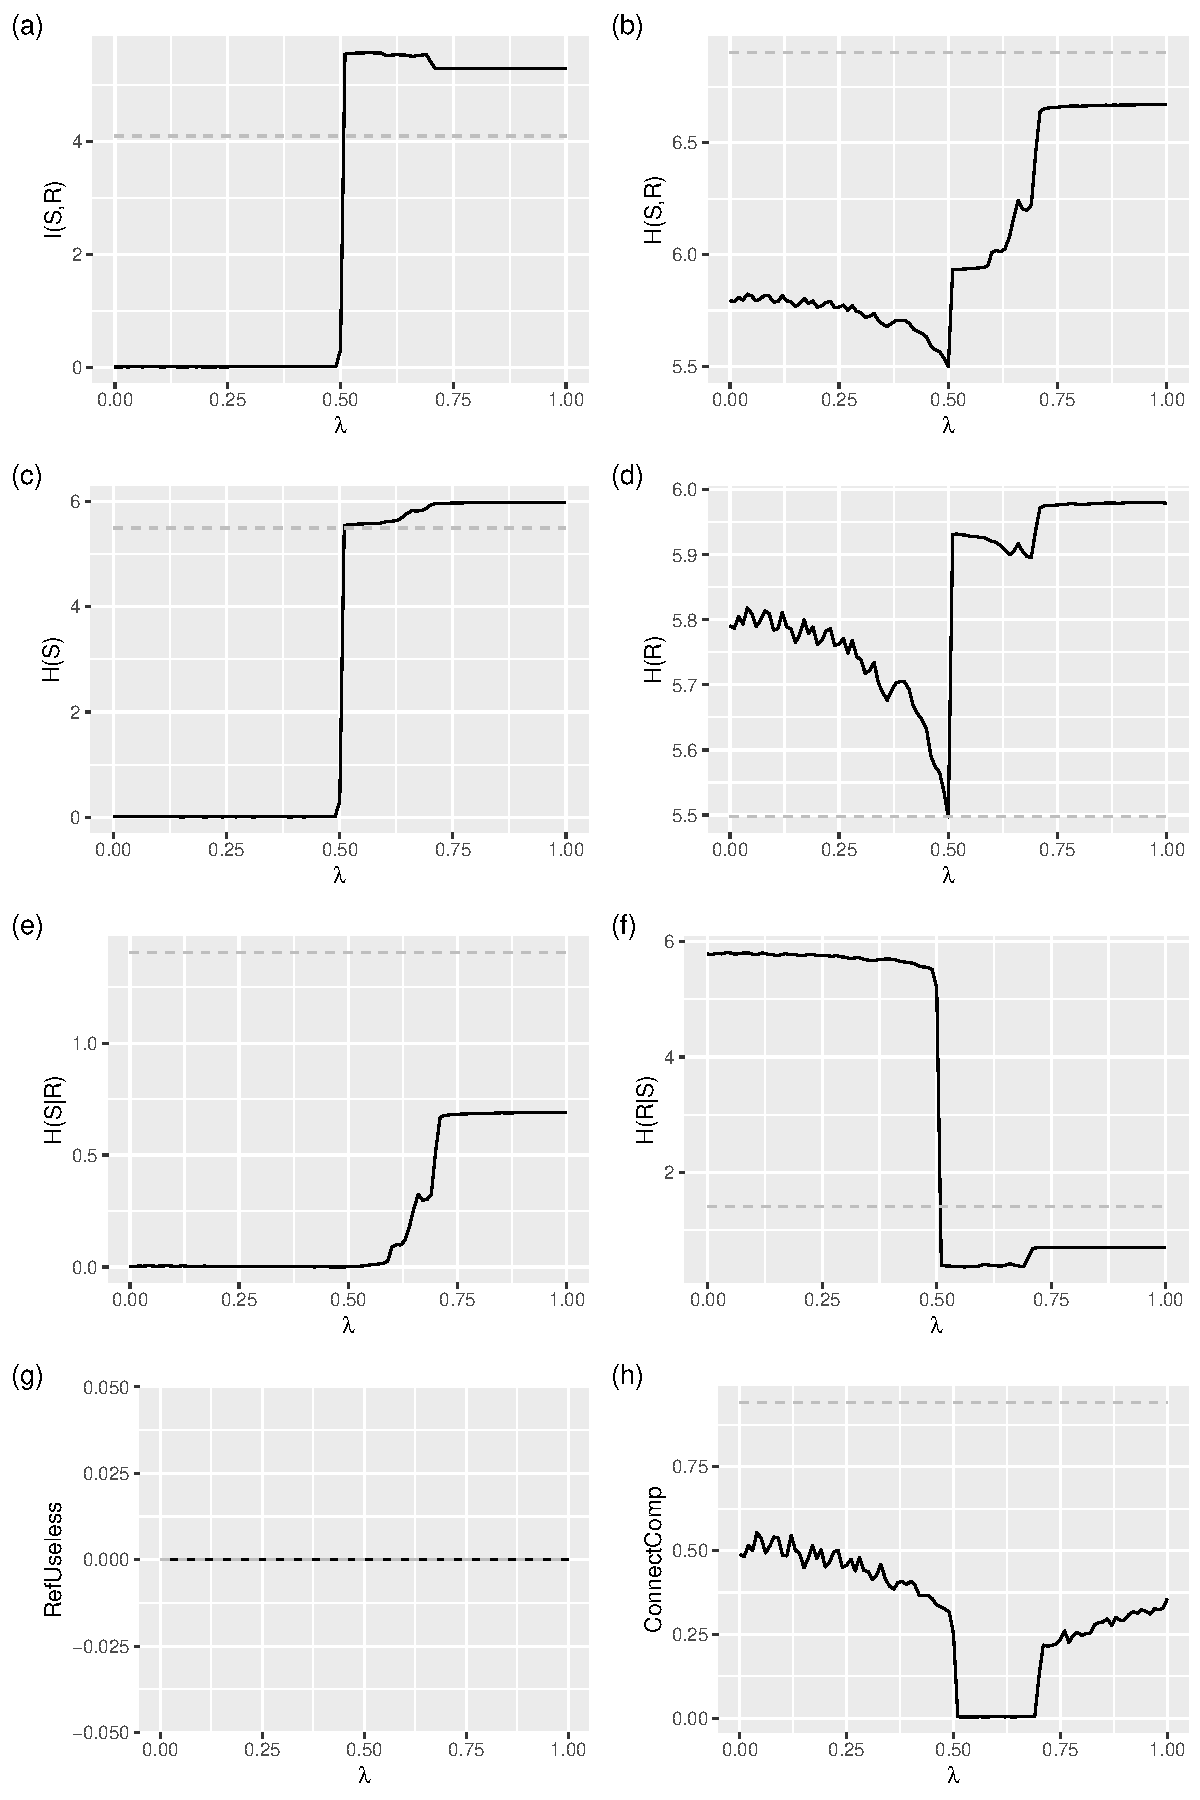
\includegraphics[width=\textwidth]{informationTheoretic_firstModel_phi1_nm400_dynamic_randomBipartite_allowUnlinked}
  \caption{a}
  \label{fig:informationTheoretic_firstModel_phi1_nm400_dynamic_randomBipartite_allowUnlinked}
\end{figure}

\begin{figure}
  \centering
  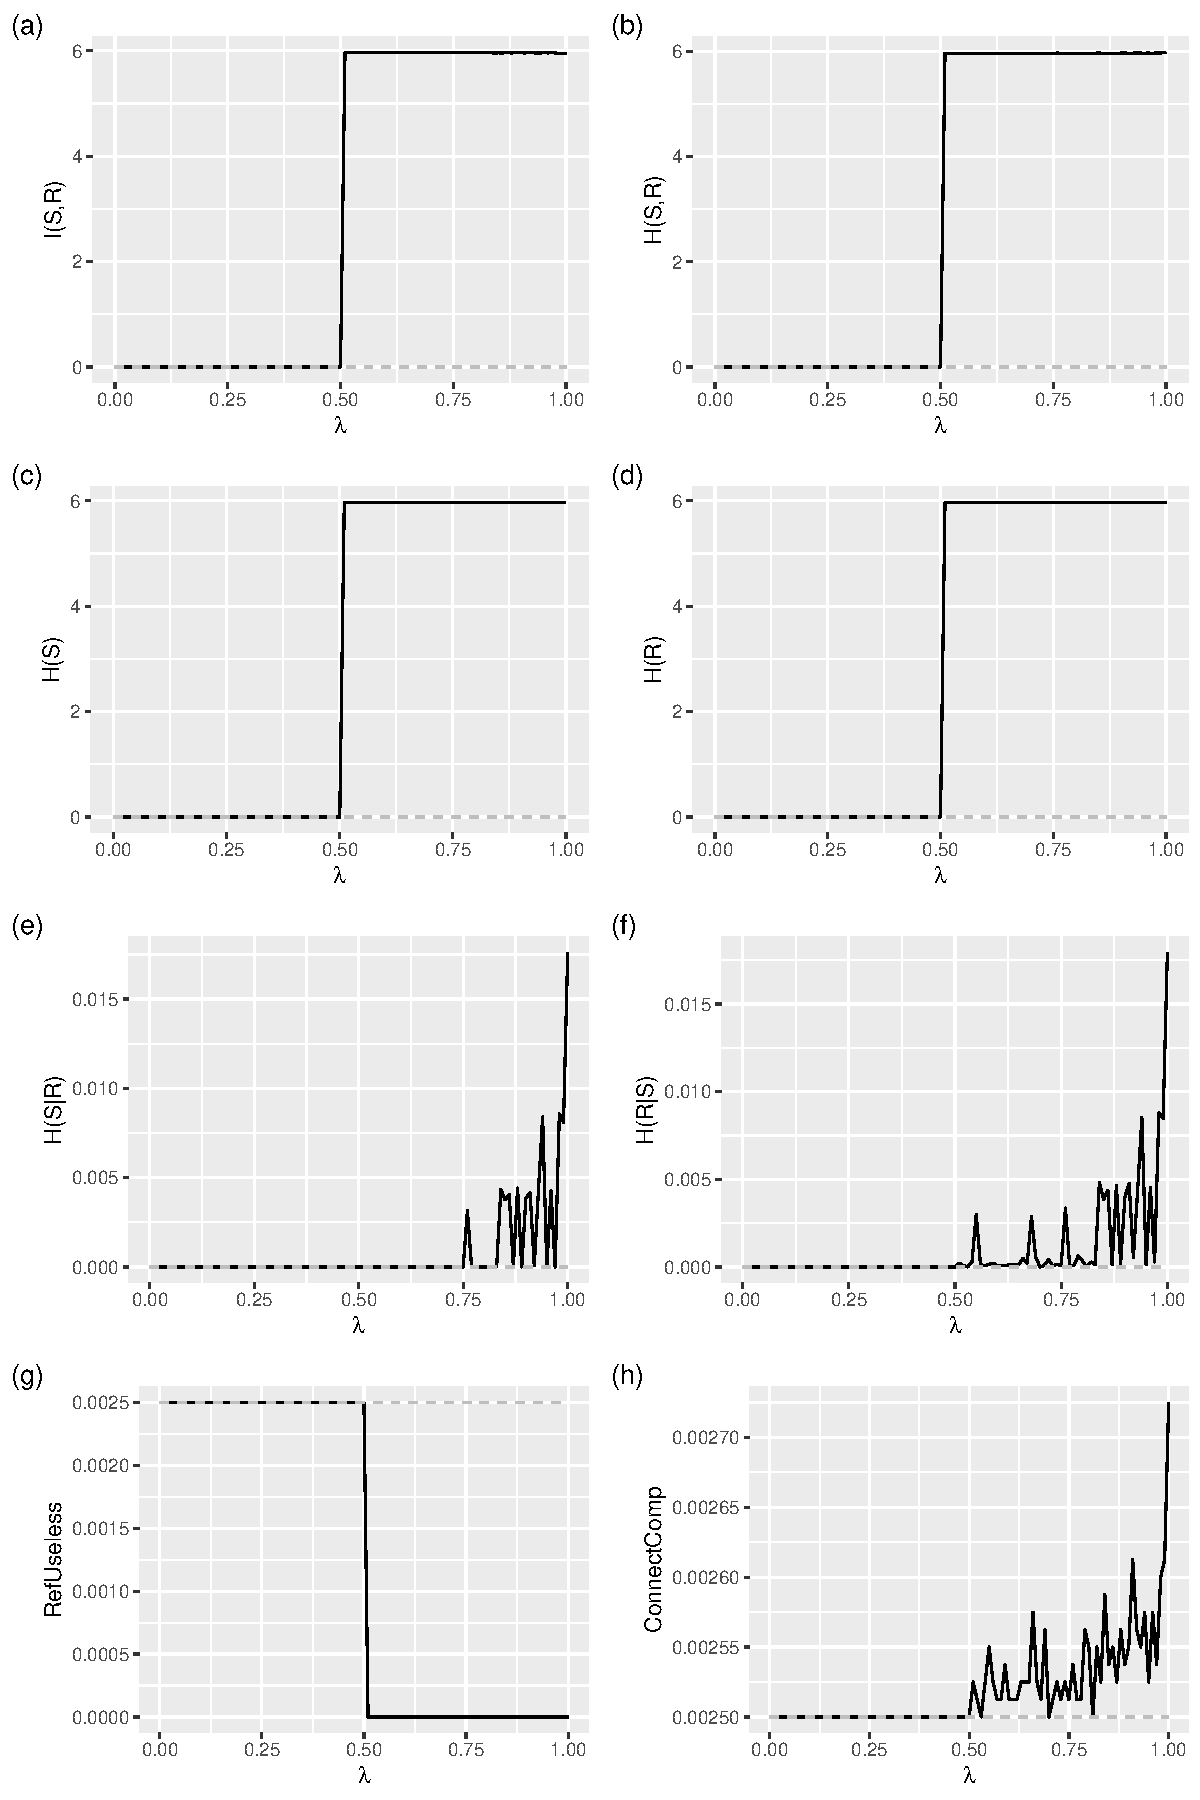
\includegraphics[width=\textwidth]{informationTheoretic_firstModel_phi1_nm400_dynamic_singleLink_allowUnlinked}
  \caption{a}
  \label{fig:informationTheoretic_firstModel_phi1_nm400_dynamic_singleLink_allowUnlinked}
\end{figure}

\begin{figure}
  \centering
  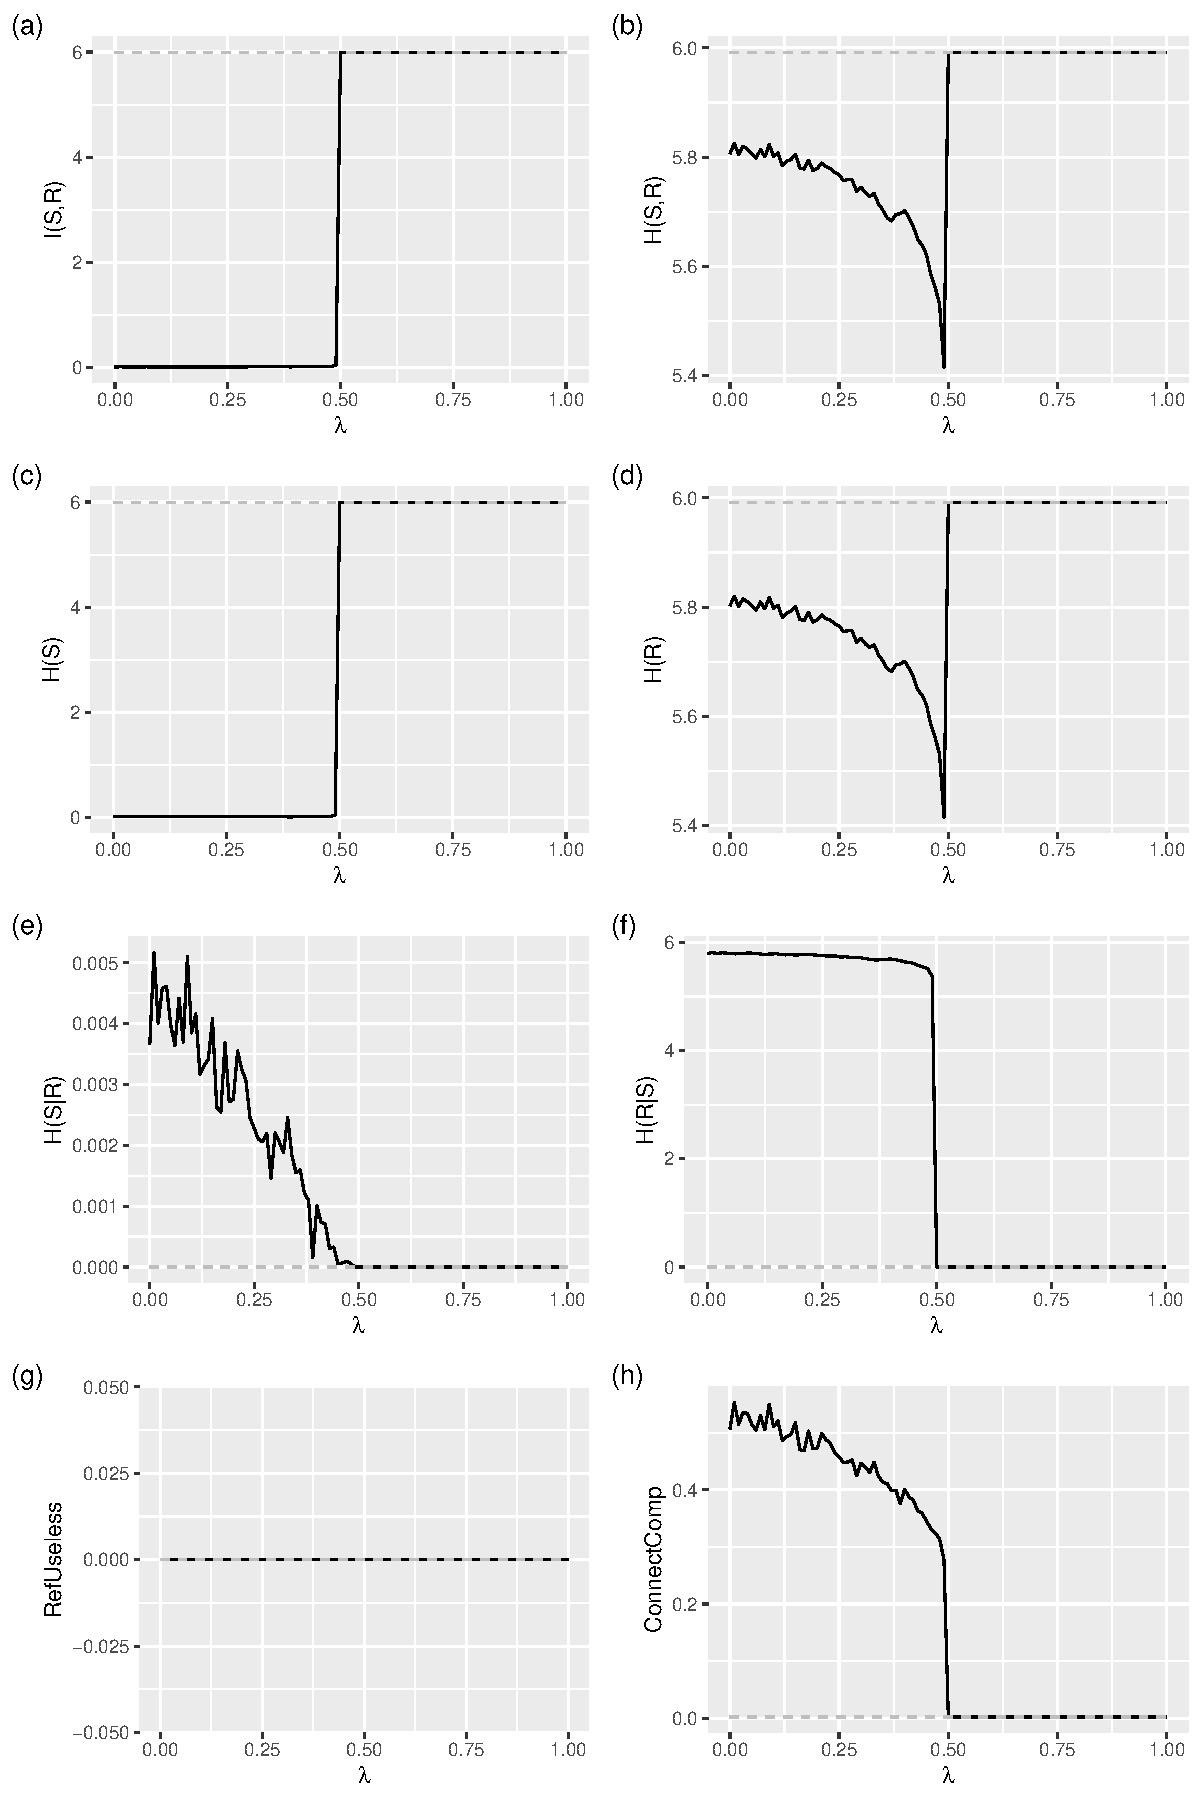
\includegraphics[width=\textwidth]{informationTheoretic_firstModel_phi1_nm400_dynamic_oneToOne_allowUnlinked}
  \caption{a}
  \label{fig:informationTheoretic_firstModel_phi1_nm400_dynamic_oneToOne_allowUnlinked}
\end{figure}

Figures \ref{fig:insideLambda_firstModel_phi1_nm400_dynamic_randomBipartite_allowUnlinked} and \ref{fig:insideLambda_firstModel_phi1_nm400_dynamic_oneToOne_allowUnlinked} (random and one-to-one initial conditions respectively) show statistical measures of select values of $\lambda$, with Figures \ref{fig:fitting_insideLambda_firstModel_phi1_nm400_dynamic_randomBipartite_allowUnlinked} and \ref{fig:fitting_insideLambda_firstModel_phi1_nm400_dynamic_oneToOne_allowUnlinked} (random and one-to-one respectively) showing the fitting of the curve to a power law for a single select value of $\lambda$ and Tables \ref{tab:fitting_insideLambda_firstModel_phi1_nm400_dynamic_randomBipartite_allowUnlinked} and \ref{tab:fitting_insideLambda_firstModel_phi1_nm400_dynamic_oneToOne_allowUnlinked} (random and one-to-one respectively) showing the values of the regression exponent and factor.
The single link initial condition is not plotted for select values of $\lambda$ as it fails to evolve beyond the single link state.

\begin{figure}
  \centering
  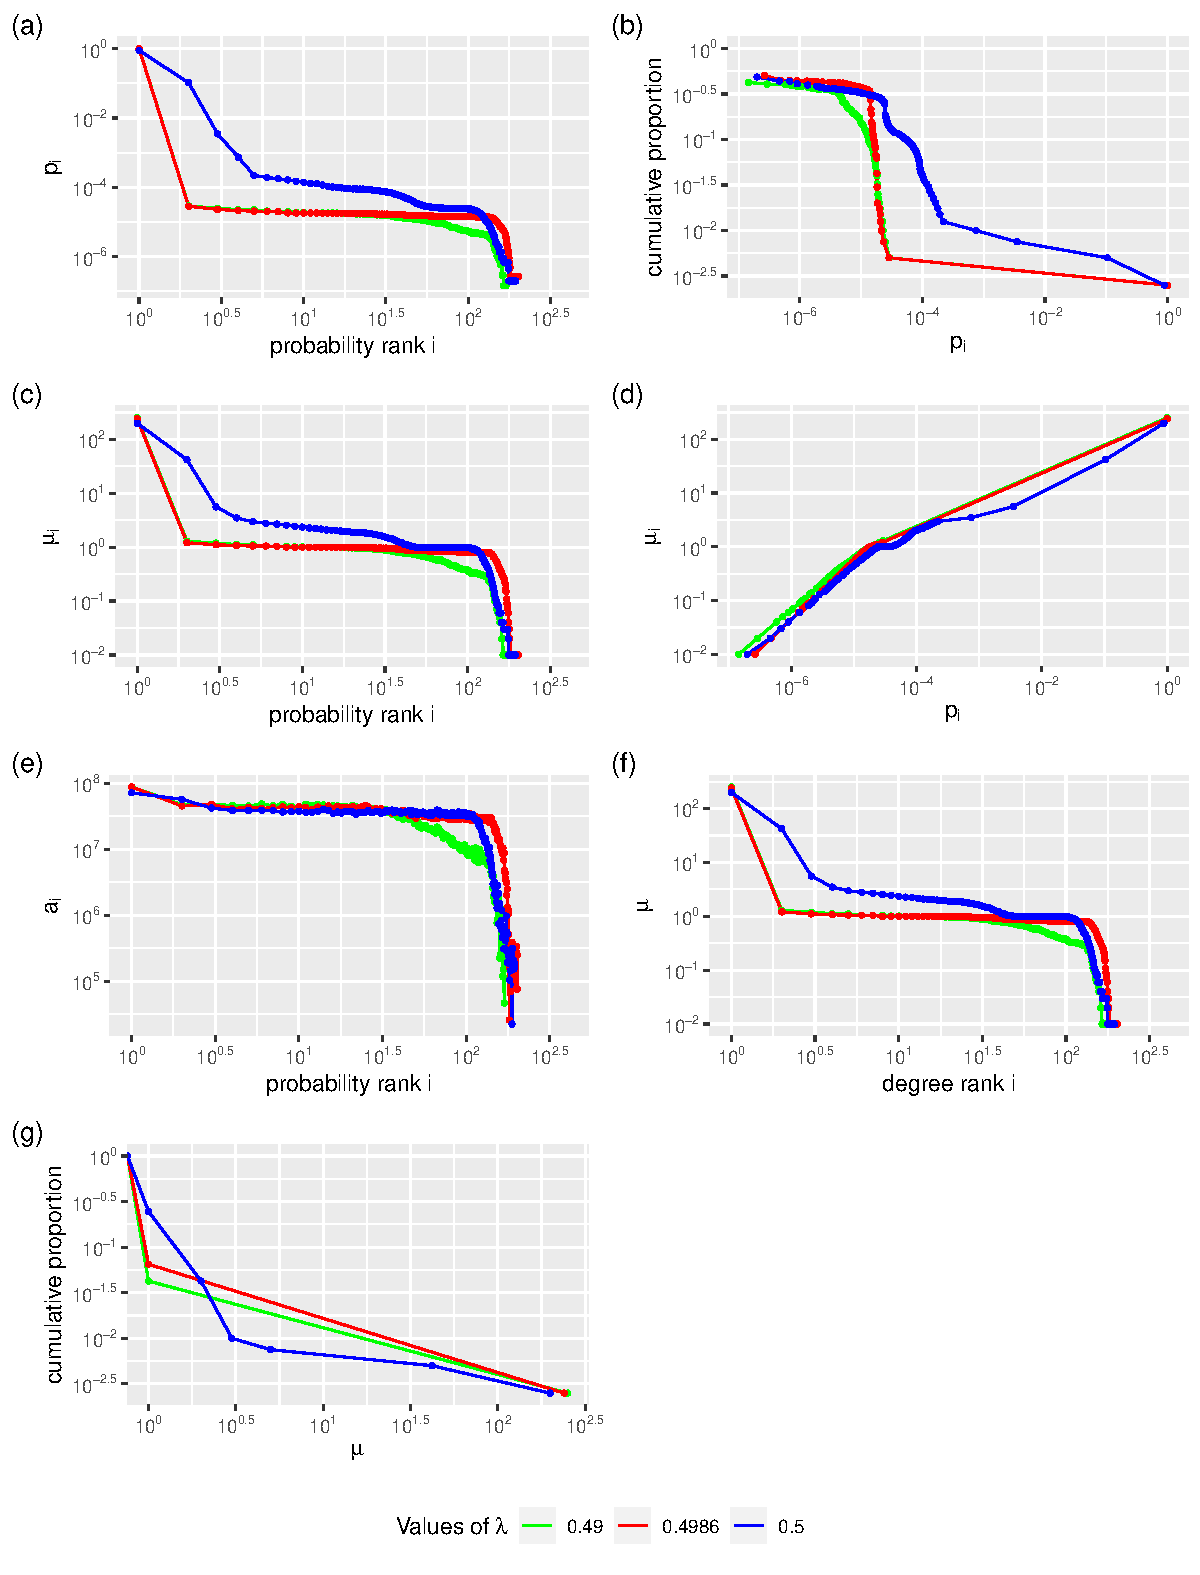
\includegraphics[width=\textwidth]{insideLambda_firstModel_phi1_nm400_dynamic_randomBipartite_allowUnlinked}
  \caption{a}
  \label{fig:insideLambda_firstModel_phi1_nm400_dynamic_randomBipartite_allowUnlinked}
\end{figure}

\begin{figure}
  \centering
  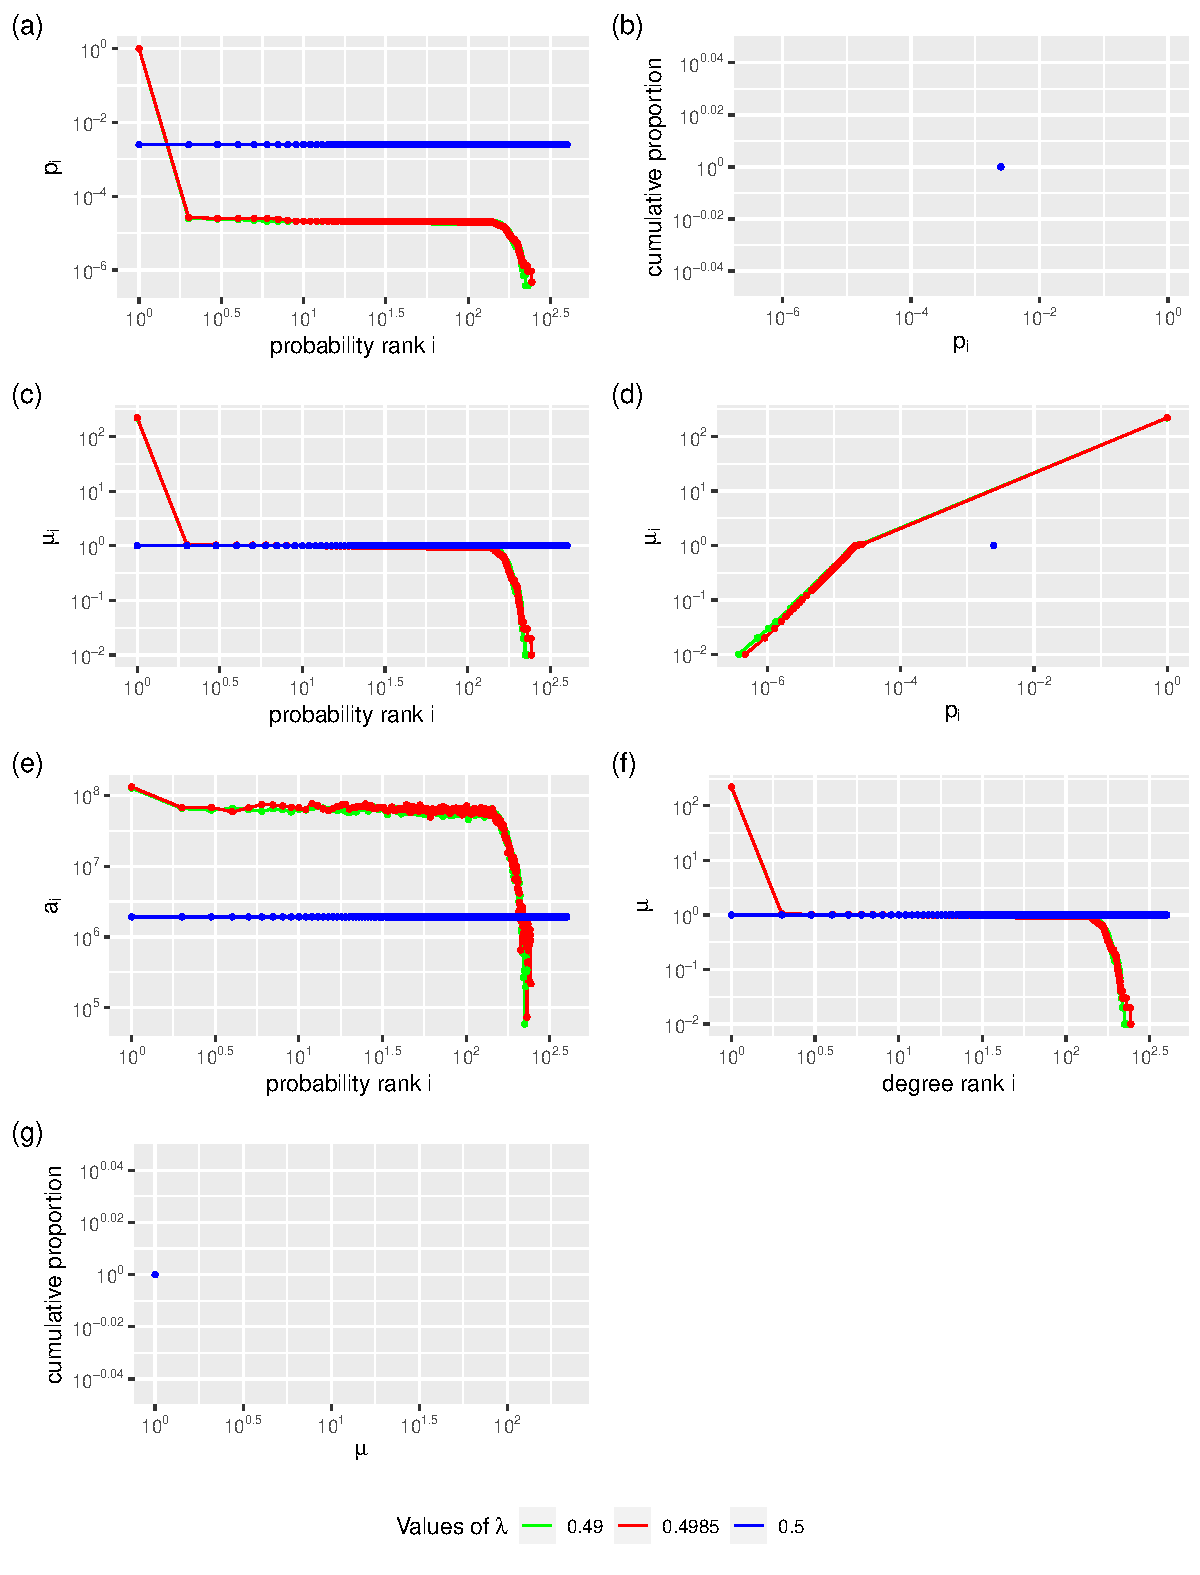
\includegraphics[width=\textwidth]{insideLambda_firstModel_phi1_nm400_dynamic_oneToOne_allowUnlinked}
  \caption{a}
  \label{fig:insideLambda_firstModel_phi1_nm400_dynamic_oneToOne_allowUnlinked}
\end{figure}

\begin{figure}
  \centering
  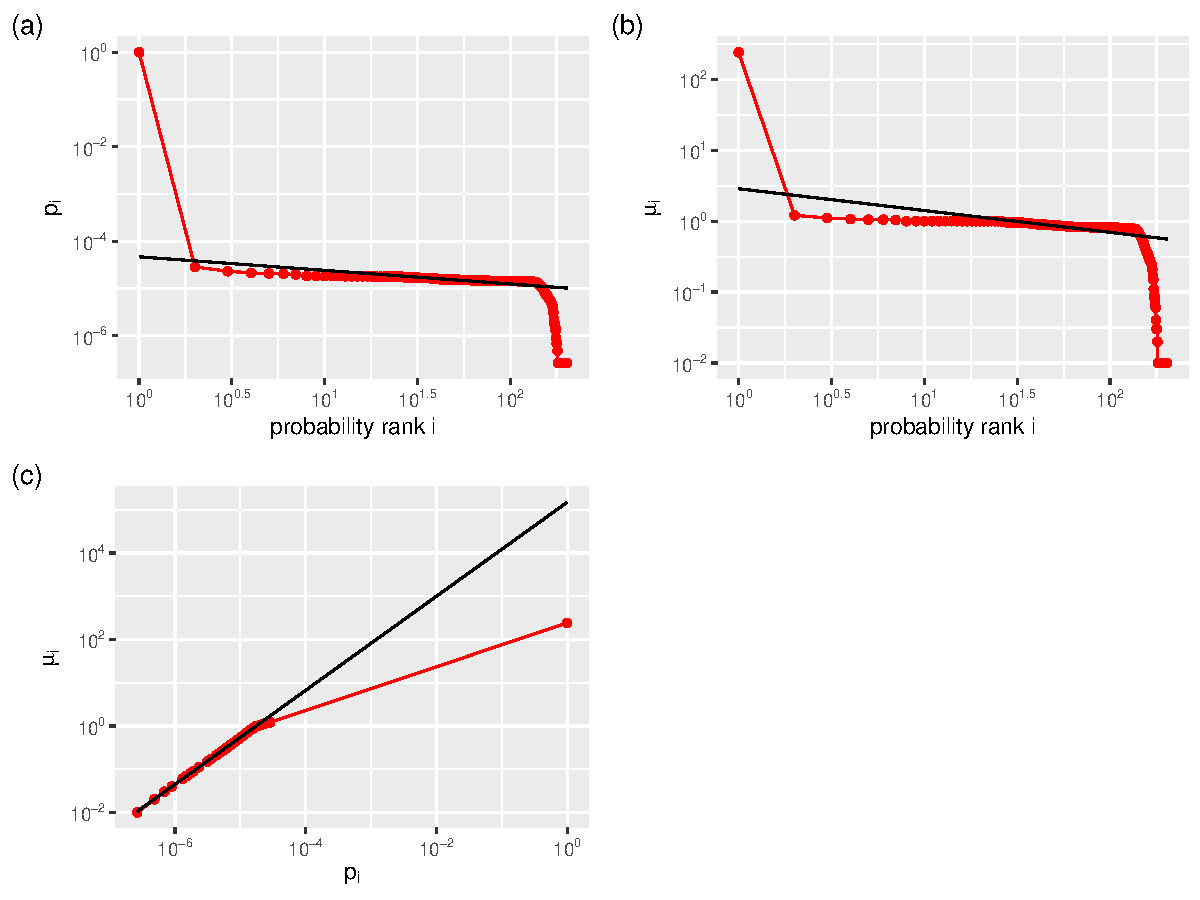
\includegraphics[width=\textwidth]{fitting_insideLambda_firstModel_phi1_nm400_dynamic_randomBipartite_allowUnlinked}
  \caption{0.4986}
  \label{fig:fitting_insideLambda_firstModel_phi1_nm400_dynamic_randomBipartite_allowUnlinked}
\end{figure}

\begin{figure}
  \centering
  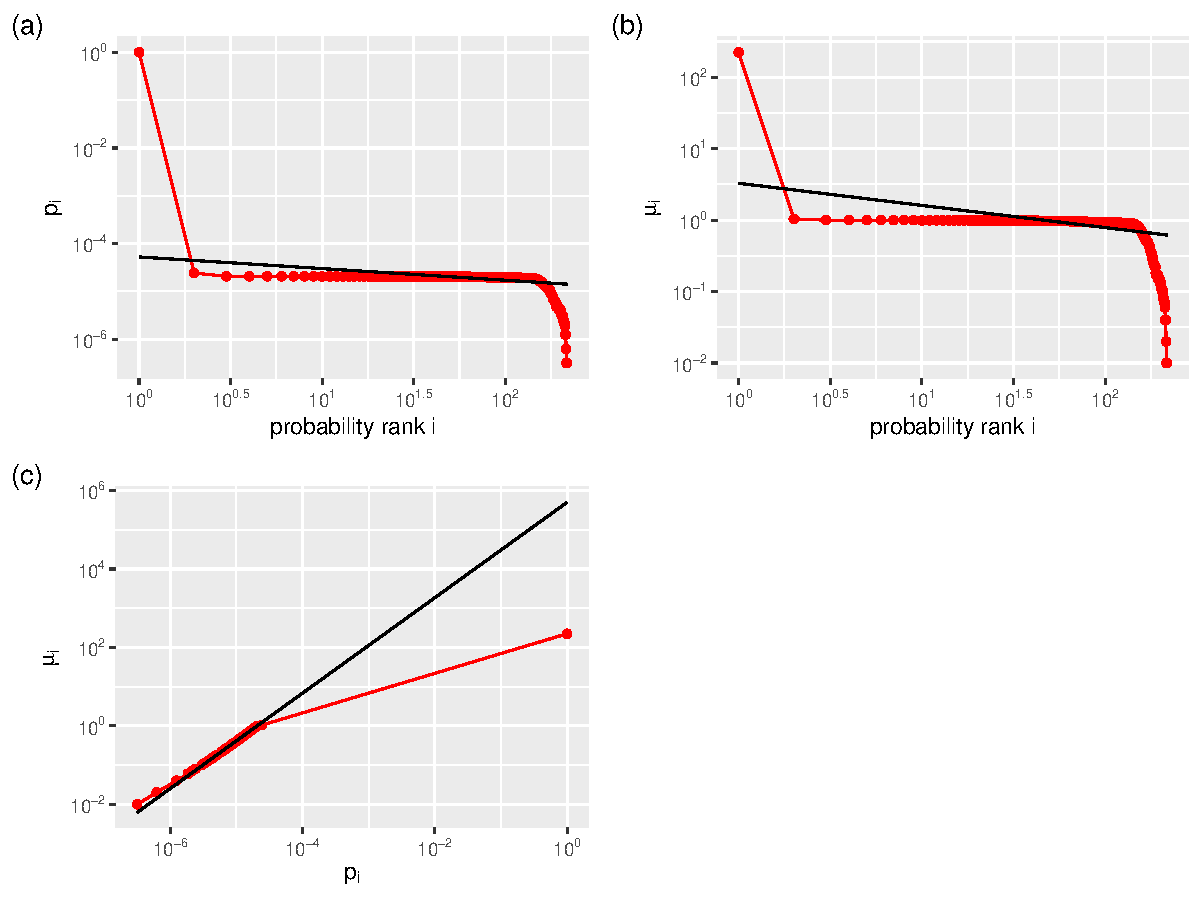
\includegraphics[width=\textwidth]{fitting_insideLambda_firstModel_phi1_nm400_dynamic_oneToOne_allowUnlinked}
  \caption{0.4993}
  \label{fig:fitting_insideLambda_firstModel_phi1_nm400_dynamic_oneToOne_allowUnlinked}
\end{figure}

% latex table generated in R 4.0.4 by xtable 1.8-4 package
% Wed Mar 17 14:32:51 2021
\begin{table}[ht]
\centering
\begin{tabular}{lrr}
  \hline
plot & alpha & k \\ 
  \hline
a & -0.2871434 & 0.0000468 \\ 
  b & -2.5493723 & 0.0000000 \\ 
  c & -0.3072861 & 2.8668125 \\ 
  d & 1.0876280 & 149669.1453764 \\ 
  f & -0.3072861 & 2.8668125 \\ 
  g & -0.5944739 & 0.0650000 \\ 
   \hline
\end{tabular}
\caption{caption} 
\label{tables/fitting_insideLambda_firstModel_phi1_nm400_dynamic_randomBipartite_allowUnlinked}
\end{table}


% latex table generated in R 4.0.4 by xtable 1.8-4 package
% Wed Mar 17 14:56:06 2021
\begin{table}[ht]
\centering
\begin{tabular}{lrr}
  \hline
plot & $\alpha$ & $k$ \\ 
  \hline
a & 0.2433438 & 0.0000524 \\ 
  b & 2.2902299 & 0.0000000 \\ 
  c & 0.3100715 & 3.2784604 \\ 
  d & -1.2166546 & 501643.7856344 \\ 
  f & 0.3100715 & 3.2784604 \\ 
  g & 0.4063538 & 0.0225000 \\ 
   \hline
\end{tabular}
\caption{Table showing the exponent and factor of the power laws fitted in Figure \ref{fig:fitting_insideLambda_firstModel_phi1_nm400_dynamic_oneToOne_allowUnlinked}} 
\label{tab:fitting_insideLambda_firstModel_phi1_nm400_dynamic_oneToOne_allowUnlinked}
\end{table}


For the \secondmodel{} with $\phi=0$ Figures  \ref{fig:informationTheoretic_uniform_phi0_nm400_dynamic_randomBipartite_allowUnlinked},  \ref{fig:informationTheoretic_uniform_phi0_nm400_dynamic_singleLink_allowUnlinked} and  \ref{fig:informationTheoretic_uniform_phi0_nm400_dynamic_oneToOne_allowUnlinked} show the information theoretic measures of the optimal graph for values of $\lambda$ ranging from 0 to 1.
They correspond to the random graph, single link and one-to-one initial graphs respectively.
Appendix \ref{sec:app_figures_second-model} shows the same figures but with disconnected meanings disallowed.

\begin{figure}
  \centering
  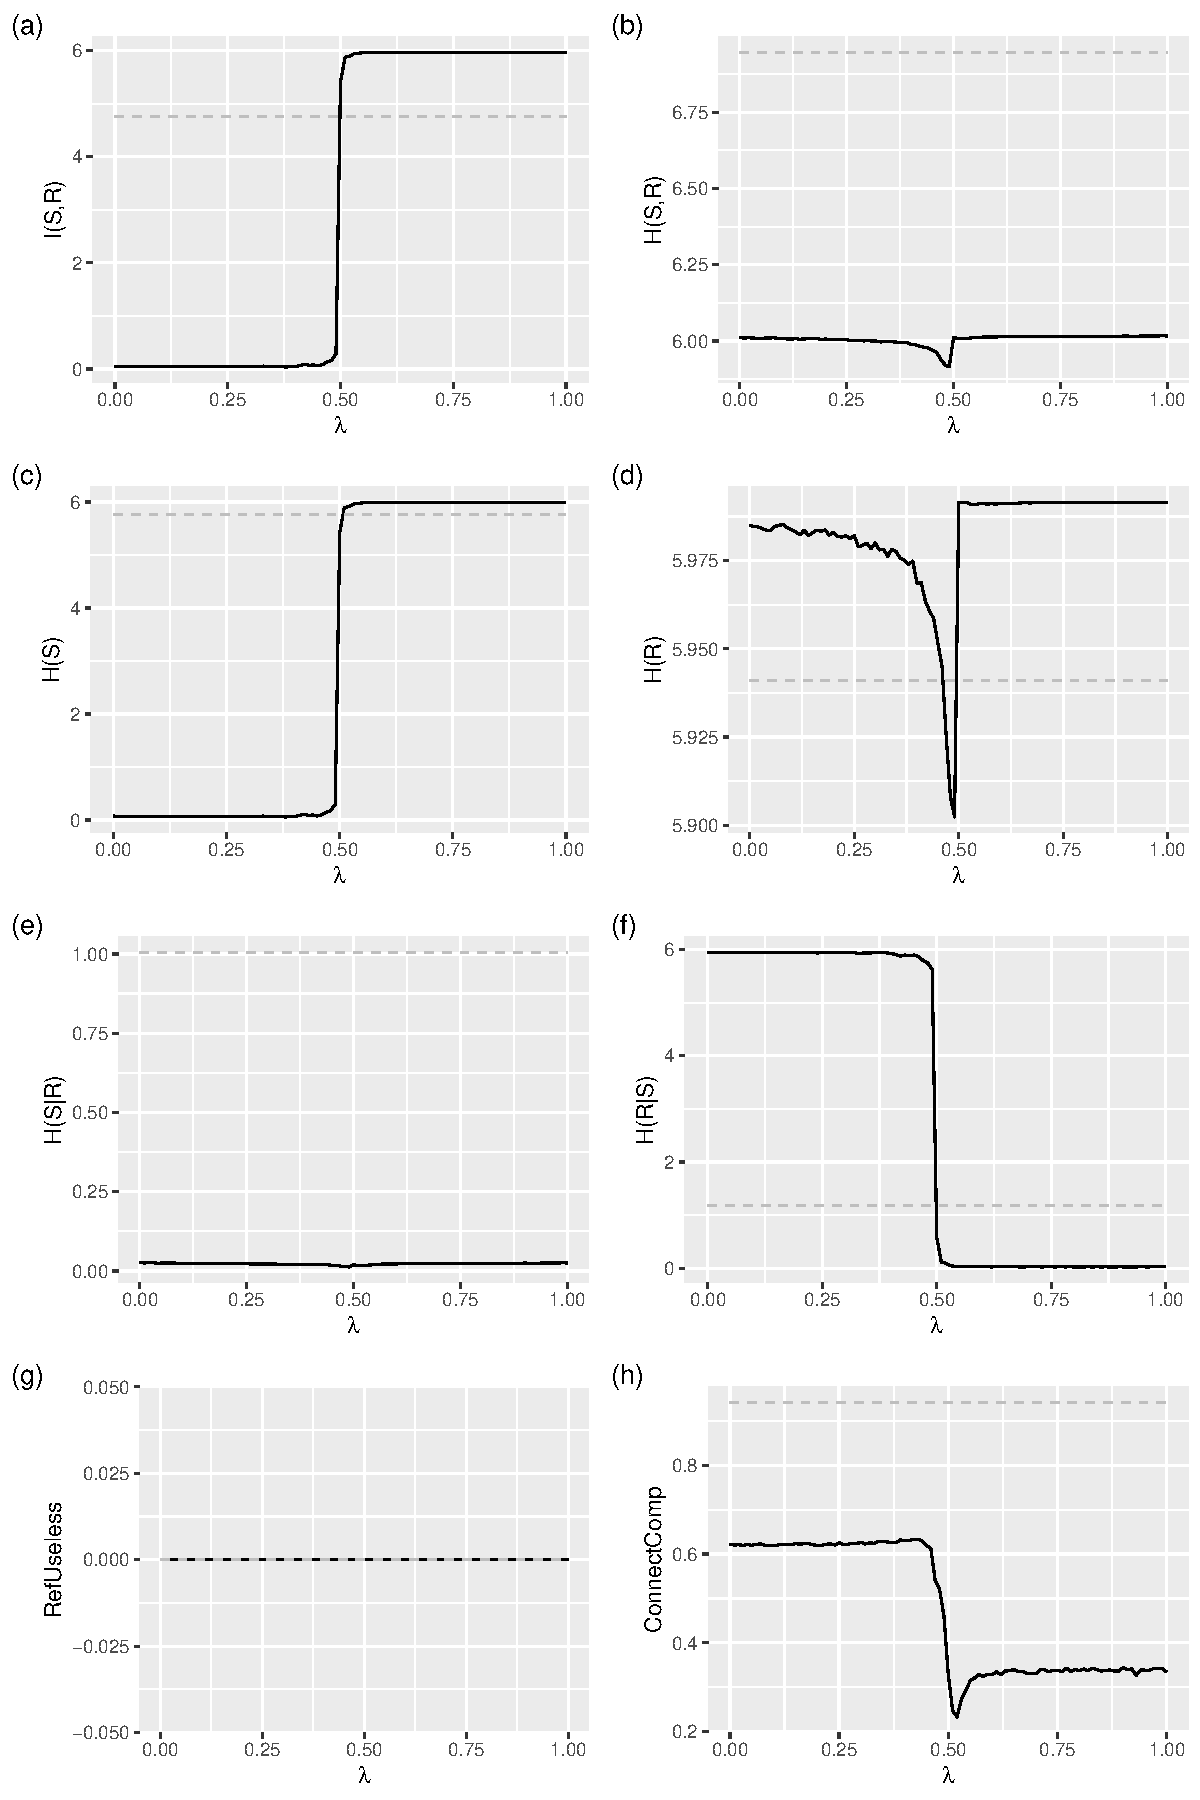
\includegraphics[width=\textwidth]{informationTheoretic_uniform_phi0_nm400_dynamic_randomBipartite_allowUnlinked}
  \caption{a}
  \label{fig:informationTheoretic_uniform_phi0_nm400_dynamic_randomBipartite_allowUnlinked}
\end{figure}

\begin{figure}
  \centering
  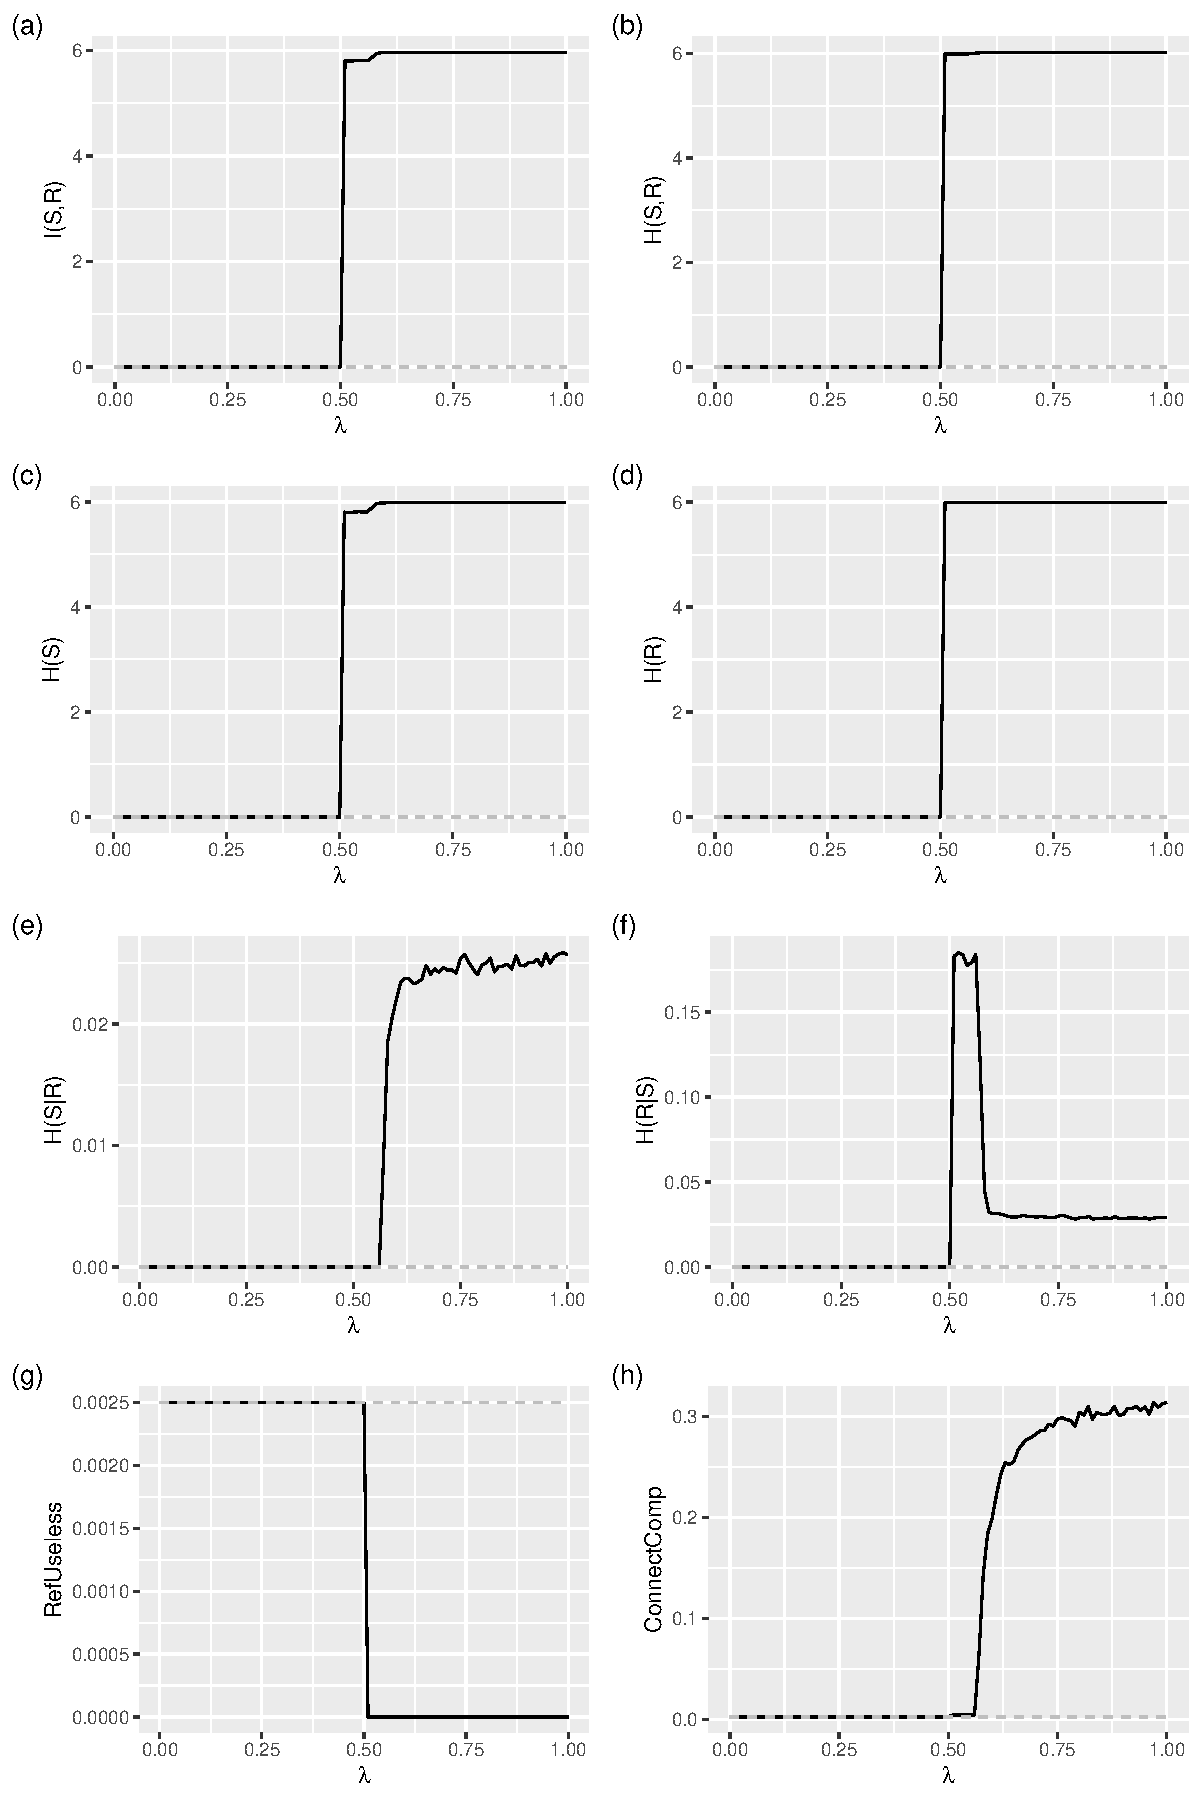
\includegraphics[width=\textwidth]{informationTheoretic_uniform_phi0_nm400_dynamic_singleLink_allowUnlinked}
  \caption{a}
  \label{fig:informationTheoretic_uniform_phi0_nm400_dynamic_singleLink_allowUnlinked}
\end{figure}

\begin{figure}
  \centering
  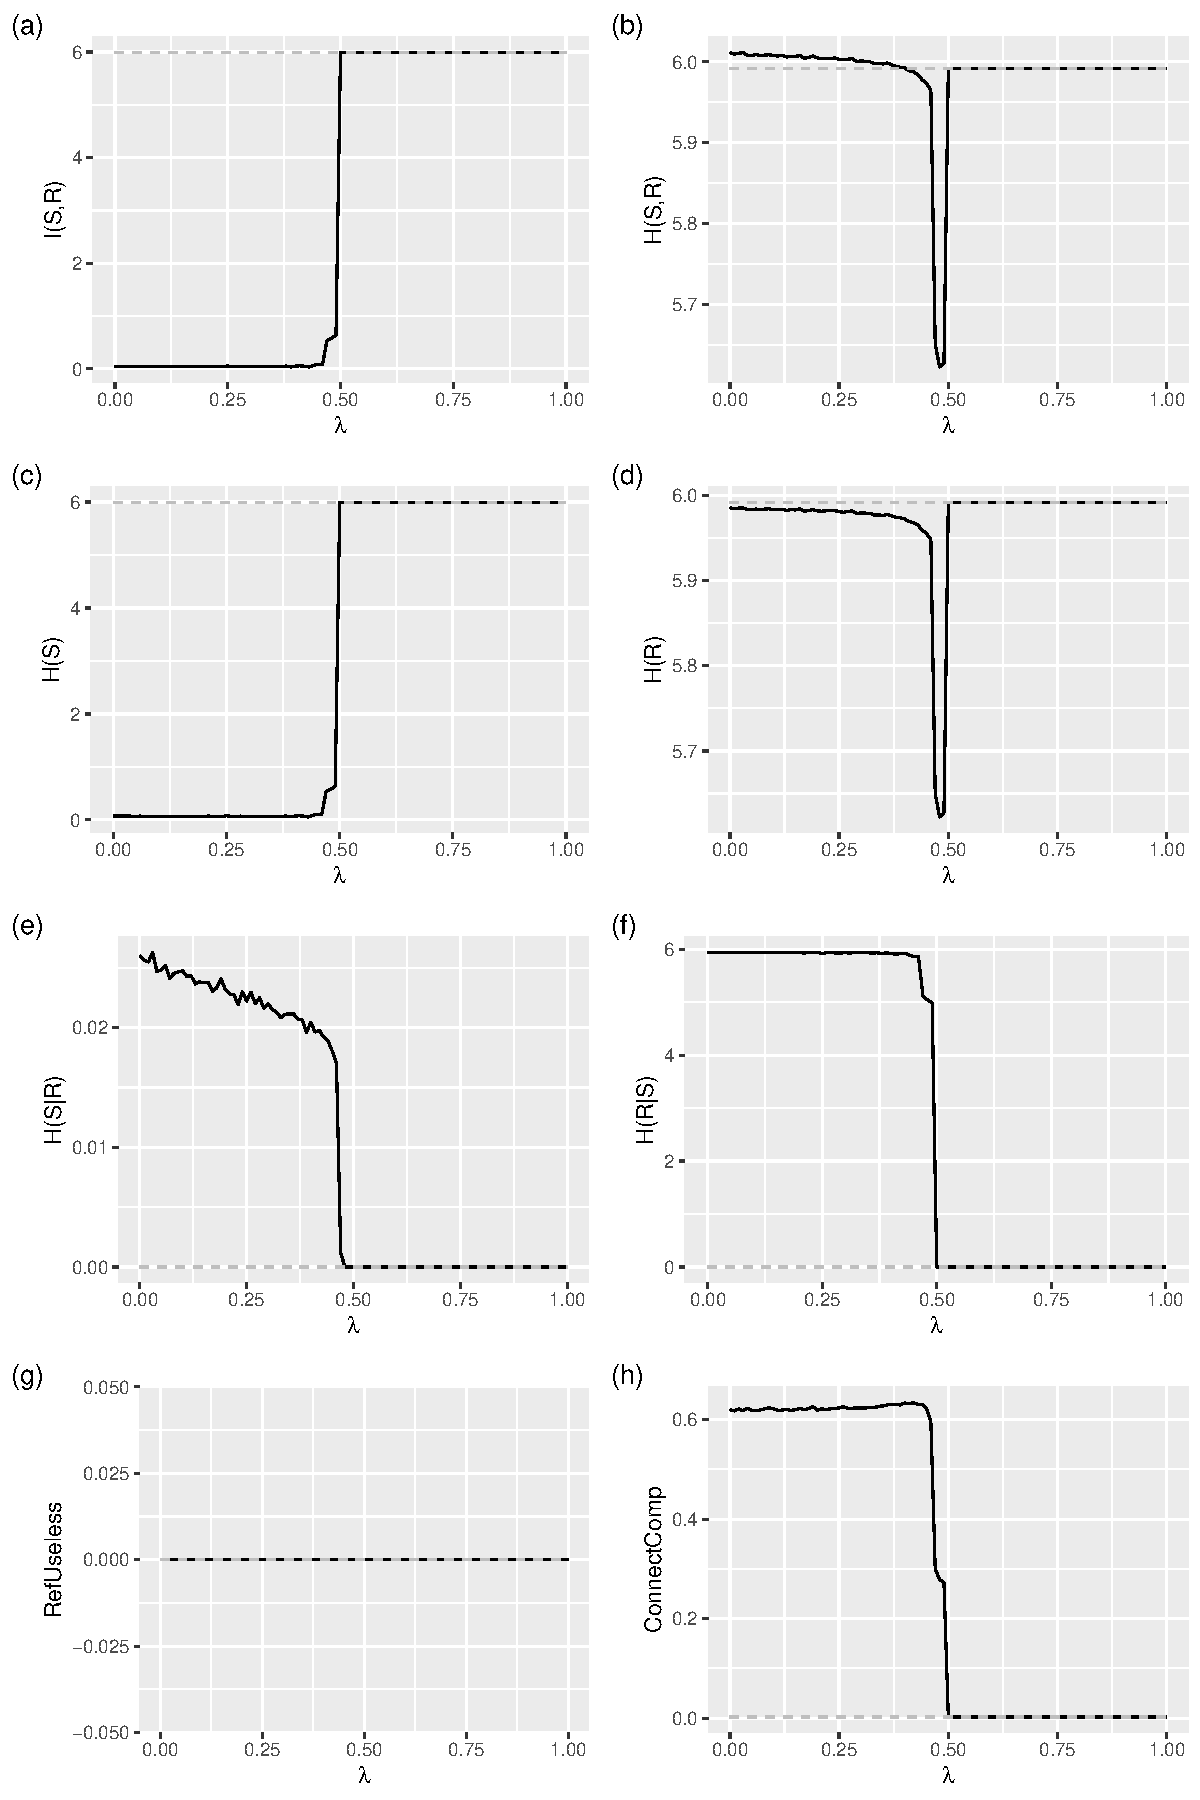
\includegraphics[width=\textwidth]{informationTheoretic_uniform_phi0_nm400_dynamic_oneToOne_allowUnlinked}
  \caption{a}
  \label{fig:informationTheoretic_uniform_phi0_nm400_dynamic_oneToOne_allowUnlinked}
\end{figure}


Figures \ref{fig:insideLambda_uniform_phi0_nm400_dynamic_randomBipartite_allowUnlinked} and \ref{fig:insideLambda_uniform_phi0_nm400_dynamic_oneToOne_allowUnlinked} (random and one-to-one respectively) show statistical measures of select values of $\lambda$, with Figures \ref{fig:fitting_insideLambda_uniform_phi0_nm400_dynamic_randomBipartite_allowUnlinked} and \ref{fig:fitting_insideLambda_uniform_phi0_nm400_dynamic_oneToOne_allowUnlinked} (random and one-to-one respectively) showing the fitting of the curve to a power law for a single select value of $\lambda$ and Tables \ref{tab:fitting_insideLambda_uniform_phi0_nm400_dynamic_randomBipartite_allowUnlinked} and \ref{tab:fitting_insideLambda_uniform_phi0_nm400_dynamic_oneToOne_allowUnlinked} (random and one-to-one respectively) showing the values of the regression exponent and factor.
As with others, the single link initial condition is not plotted for select values of $\lambda$ as it fails to evolve beyond the single link state.
Appendix \ref{sec:app_figures_second-model} shows the same figures but with disconnected meanings disallowed.

\begin{figure}
  \centering
  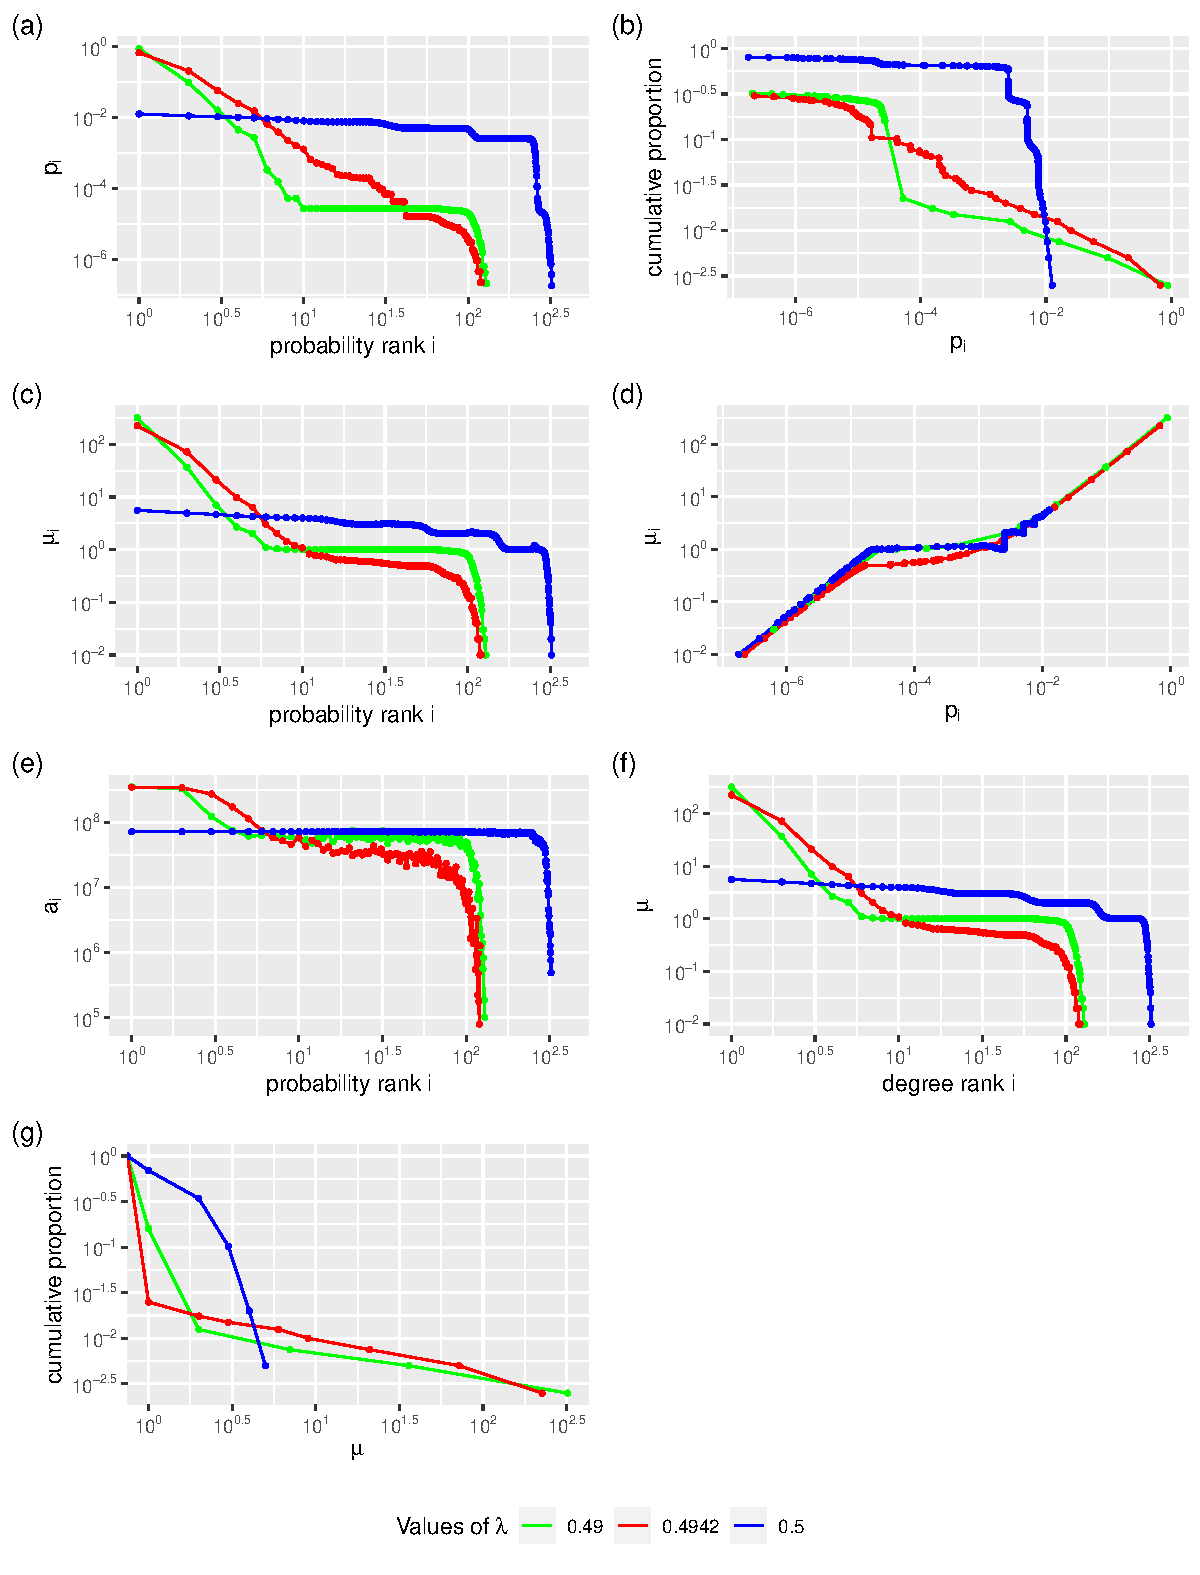
\includegraphics[width=\textwidth]{insideLambda_uniform_phi0_nm400_dynamic_randomBipartite_allowUnlinked}
  \caption{0.4942}
  \label{fig:insideLambda_uniform_phi0_nm400_dynamic_randomBipartite_allowUnlinked}
\end{figure}

\begin{figure}
  \centering
  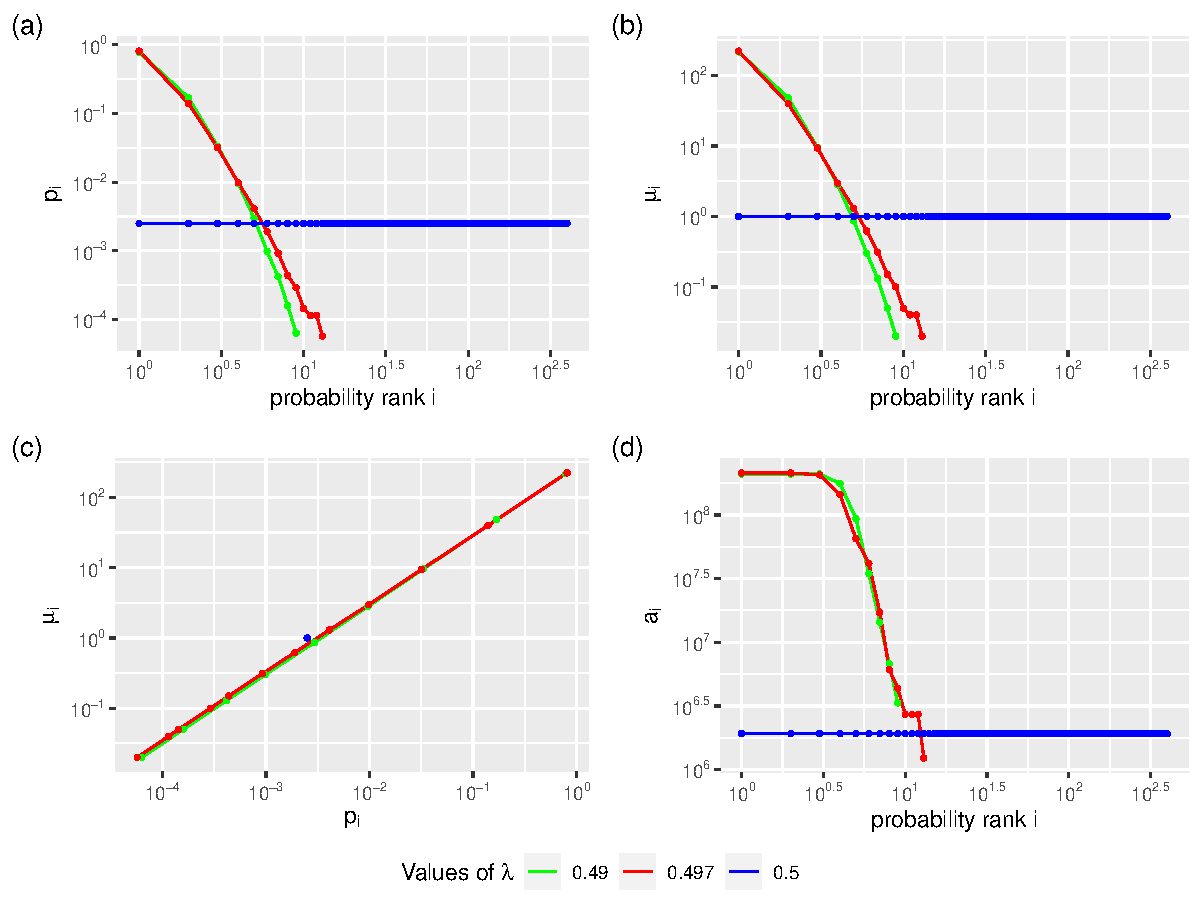
\includegraphics[width=\textwidth]{insideLambda_uniform_phi0_nm400_dynamic_oneToOne_allowUnlinked.pdf}
  \caption{0.4970}
  \label{fig:insideLambda_uniform_phi0_nm400_dynamic_oneToOne_allowUnlinked}
\end{figure}

\begin{figure}
  \centering
  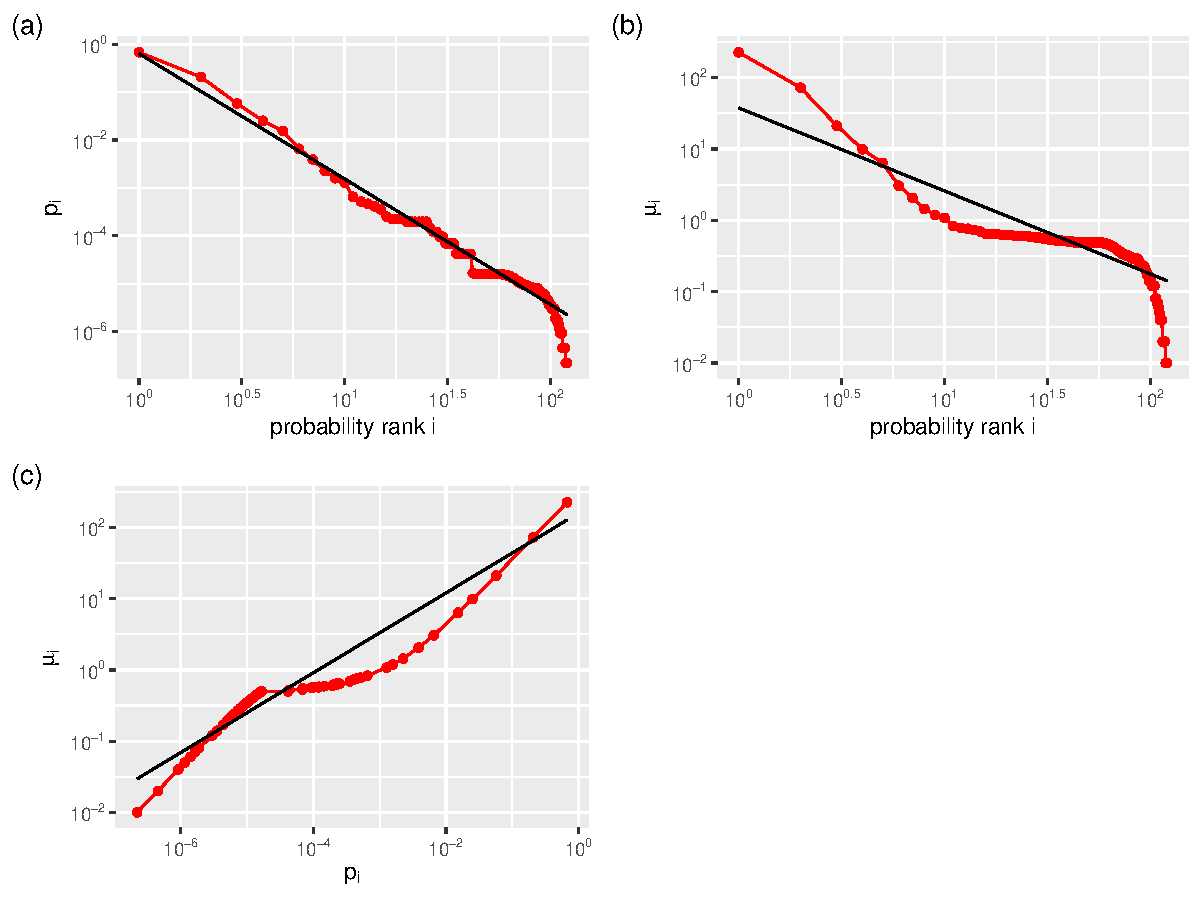
\includegraphics[width=\textwidth]{fitting_insideLambda_uniform_phi0_nm400_dynamic_randomBipartite_allowUnlinked}
  \caption{0.4942}
  \label{fig:fitting_insideLambda_uniform_phi0_nm400_dynamic_randomBipartite_allowUnlinked}
\end{figure}

\begin{figure}
  \centering
  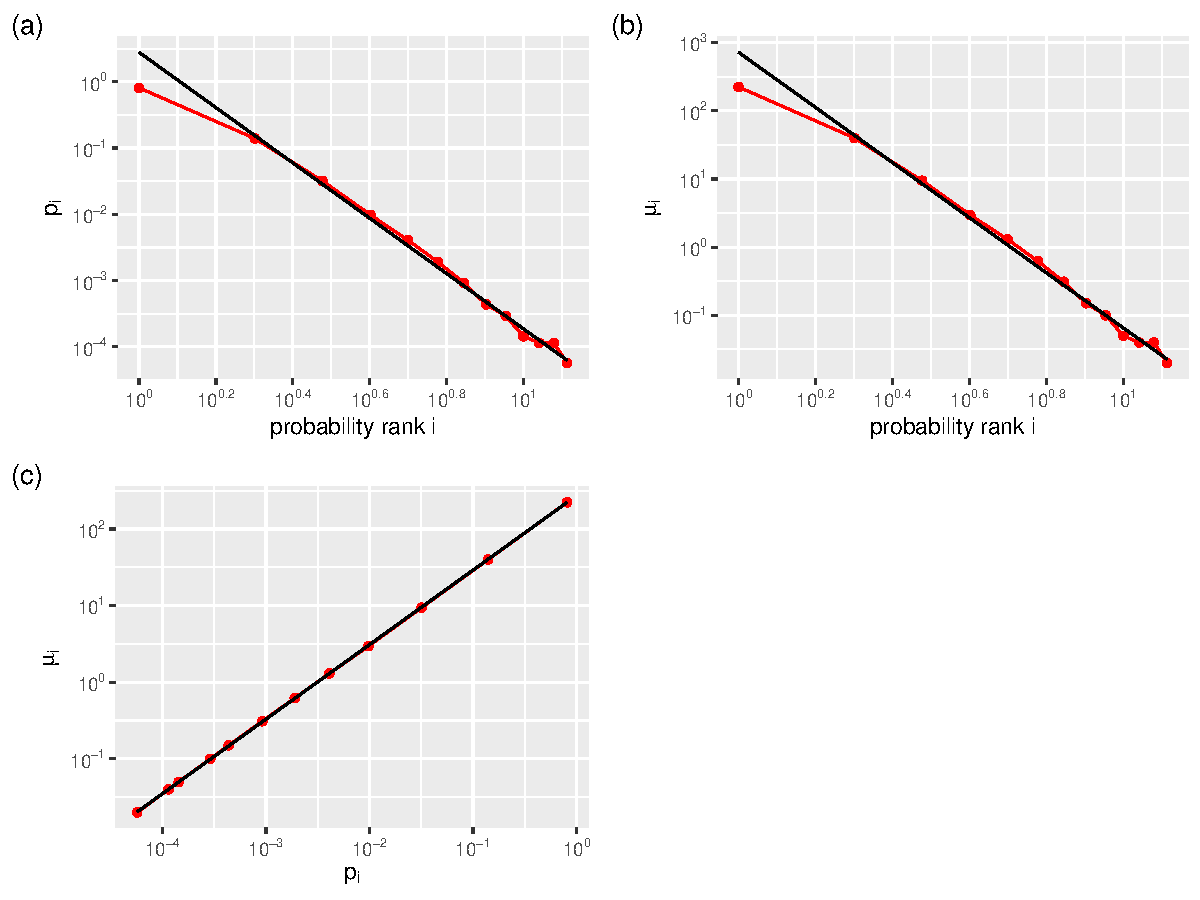
\includegraphics[width=\textwidth]{fitting_insideLambda_uniform_phi0_nm400_dynamic_oneToOne_allowUnlinked}
  \caption{0.4970}
  \label{fig:fitting_insideLambda_uniform_phi0_nm400_dynamic_oneToOne_allowUnlinked}
\end{figure}

% latex table generated in R 4.1.1 by xtable 1.8-4 package
% Sat Oct  2 23:05:07 2021
\begin{table}[ht]
\centering
\begin{tabular}{lrr}
  \hline
plot & $\alpha$ & $k$ \\ 
  \hline
a & 2.6176507 & 0.6341345 \\ 
  b & 0.3812498 & 0.0021506 \\ 
  c & 1.1623482 & 37.4616016 \\ 
  d & -0.5600378 & 158.5629462 \\ 
  f & 1.1623482 & 37.4616016 \\ 
  g & 0.3954554 & 0.0250000 \\ 
   \hline
\end{tabular}
\caption{Table showing the exponent and factor of the power laws fitted in Figure \ref{fig:fitting_insideLambda_uniform_phi0_nm400_dynamic_randomBipartite_allowUnlinked}} 
\label{tab:fitting_insideLambda_uniform_phi0_nm400_dynamic_randomBipartite_allowUnlinked}
\end{table}


% latex table generated in R 4.1.1 by xtable 1.8-4 package
% Sun Oct  3 00:21:42 2021
\begin{table}[ht]
\centering
\begin{tabular}{lrr}
  \hline
plot & $\alpha$ & $k$ \\ 
  \hline
a & 4.1719196 & 2.7845870 \\ 
  b & 0.2458167 & 0.0031418 \\ 
  c & 4.0408414 & 717.6995365 \\ 
  d & -0.9728453 & 272.7810669 \\ 
  f & 4.0408414 & 717.6995365 \\ 
  g & 0.2854165 & 0.0125000 \\ 
   \hline
\end{tabular}
\caption{Table showing the exponent and factor of the power laws fitted in Figure \ref{fig:fitting_insideLambda_uniform_phi0_nm400_dynamic_oneToOne_allowUnlinked}} 
\label{tab:fitting_insideLambda_uniform_phi0_nm400_dynamic_oneToOne_allowUnlinked}
\end{table}


For the \secondmodel{} and $\phi=1$ Figures \ref{fig:informationTheoretic_uniform_phi1_nm400_dynamic_randomBipartite_allowUnlinked},  \ref{fig:informationTheoretic_uniform_phi1_nm400_dynamic_singleLink_allowUnlinked} and \ref{fig:informationTheoretic_uniform_phi1_nm400_dynamic_oneToOne_allowUnlinked} show the information theoretic measures of the optimal graph for values of $\lambda$ ranging from 0 to 1.
They correspond to the random graph, single link and one-to-one initial graphs respectively.
Appendix \ref{sec:app_figures_second-model} also shows the same figures but with disconnected meanings disallowed.

\begin{figure}
  \centering
  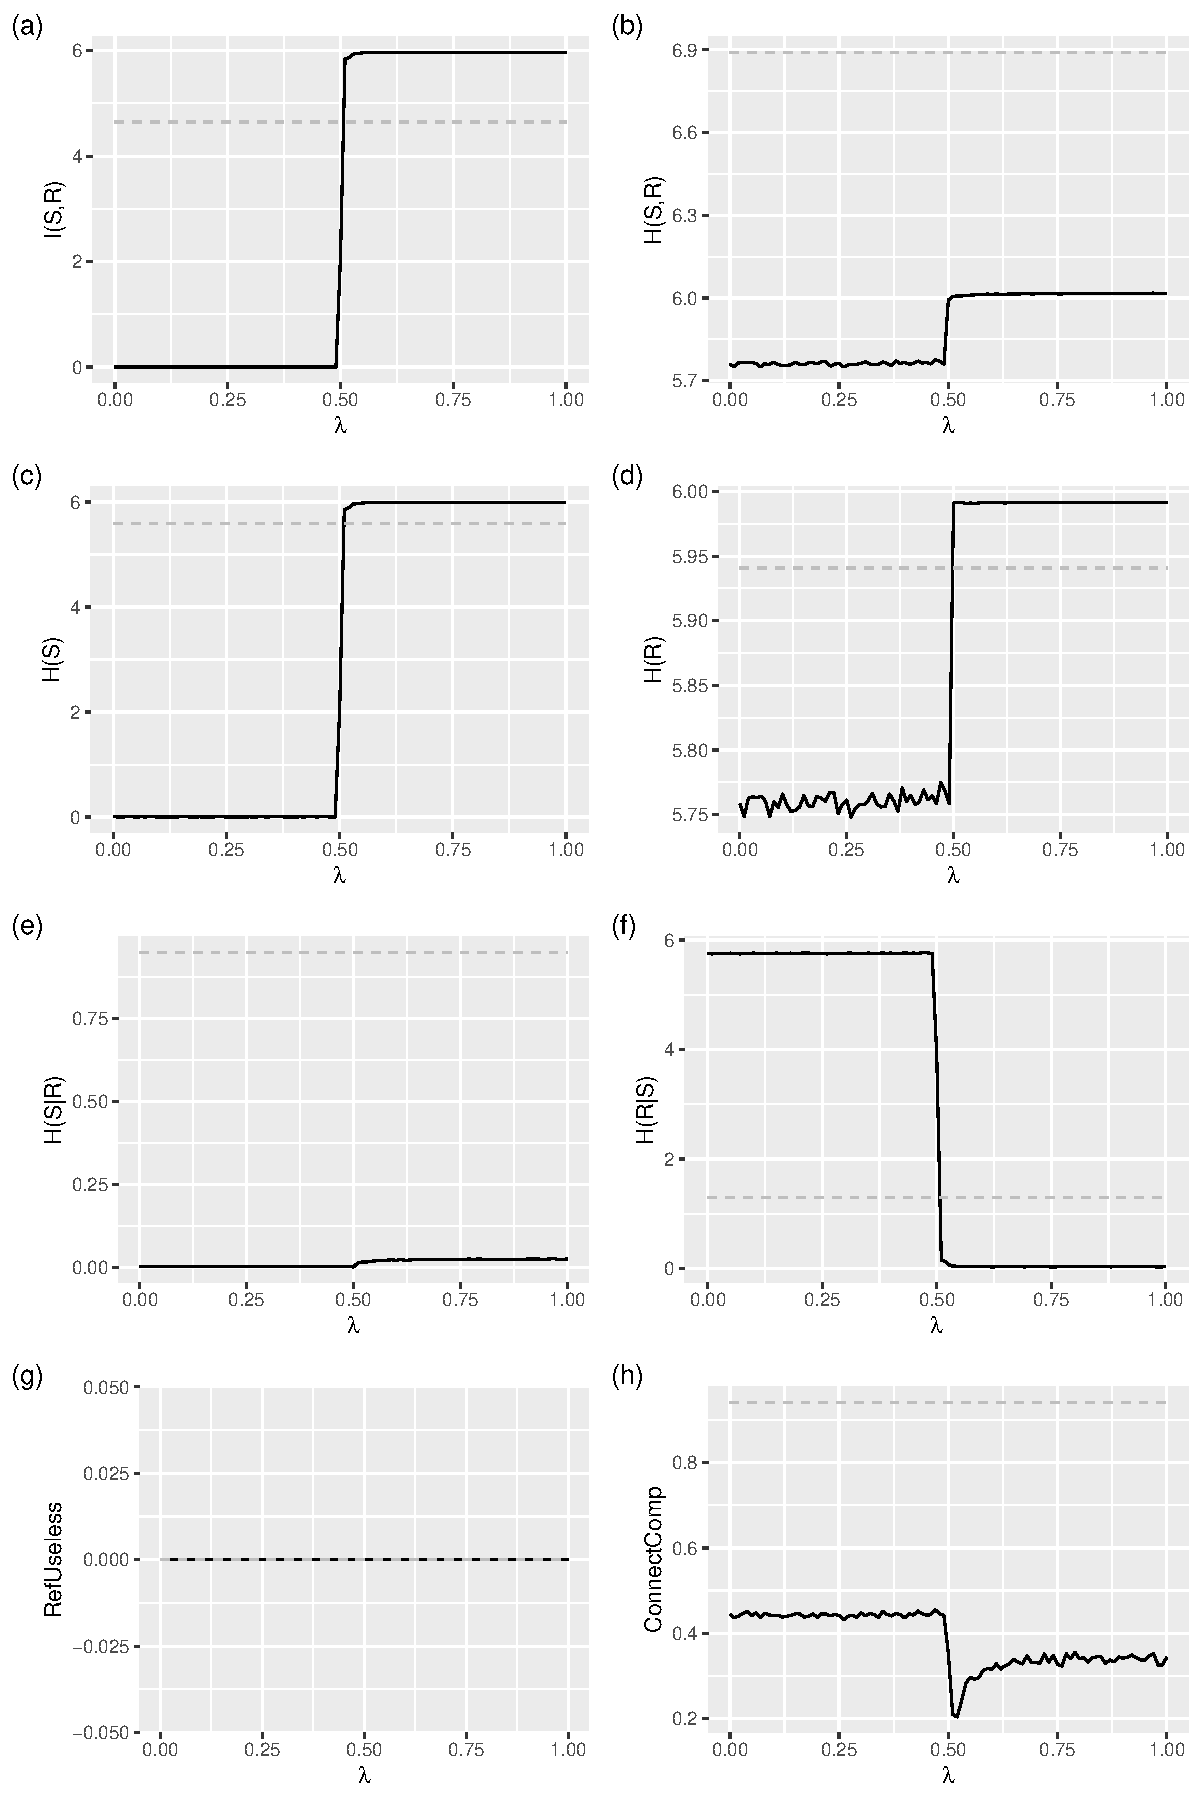
\includegraphics[width=\textwidth]{informationTheoretic_uniform_phi1_nm400_dynamic_randomBipartite_allowUnlinked}
  \caption{a}
  \label{fig:informationTheoretic_uniform_phi1_nm400_dynamic_randomBipartite_allowUnlinked}
\end{figure}

\begin{figure}
  \centering
  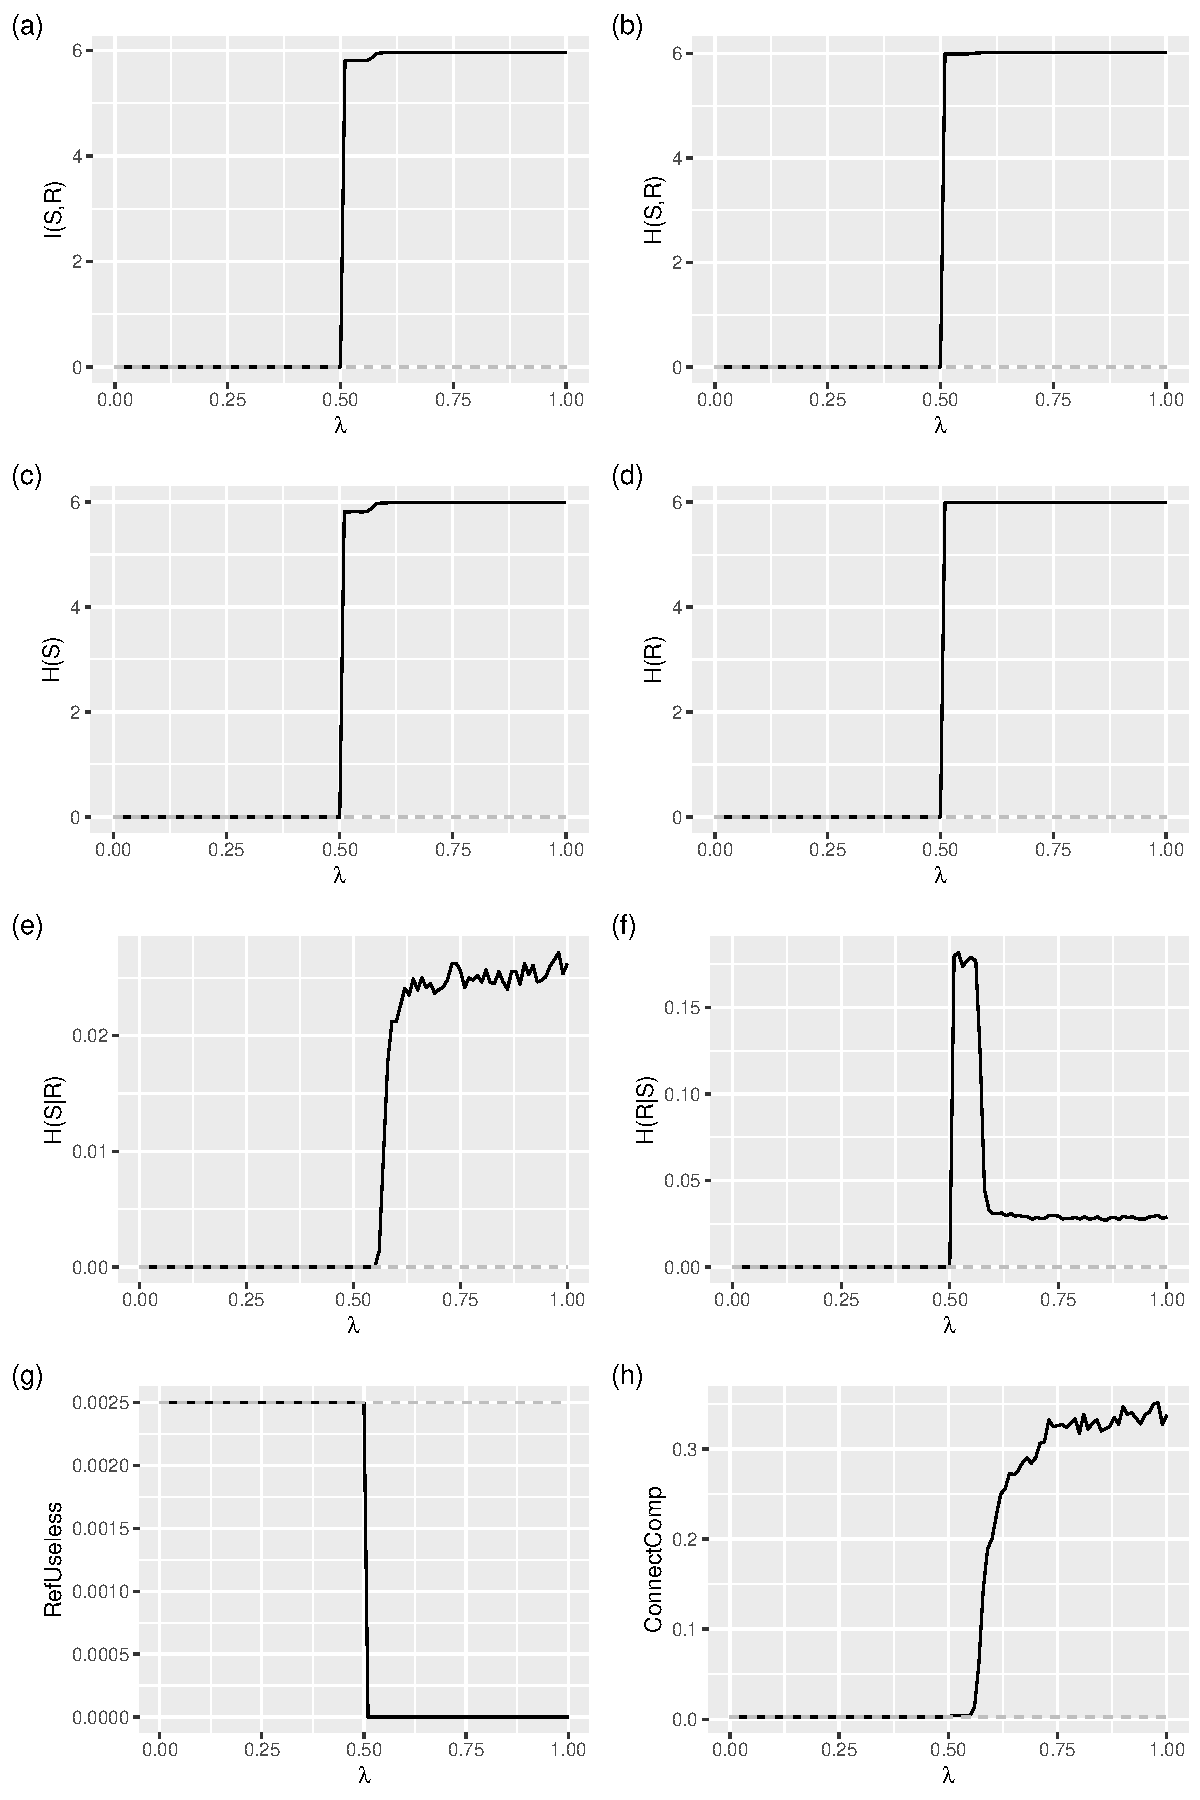
\includegraphics[width=\textwidth,draft]{informationTheoretic_uniform_phi1_nm400_dynamic_singleLink_allowUnlinked.pdf}
  \caption{a}
  \label{fig:informationTheoretic_uniform_phi1_nm400_dynamic_singleLink_allowUnlinked}
\end{figure}

\begin{figure}
  \centering
  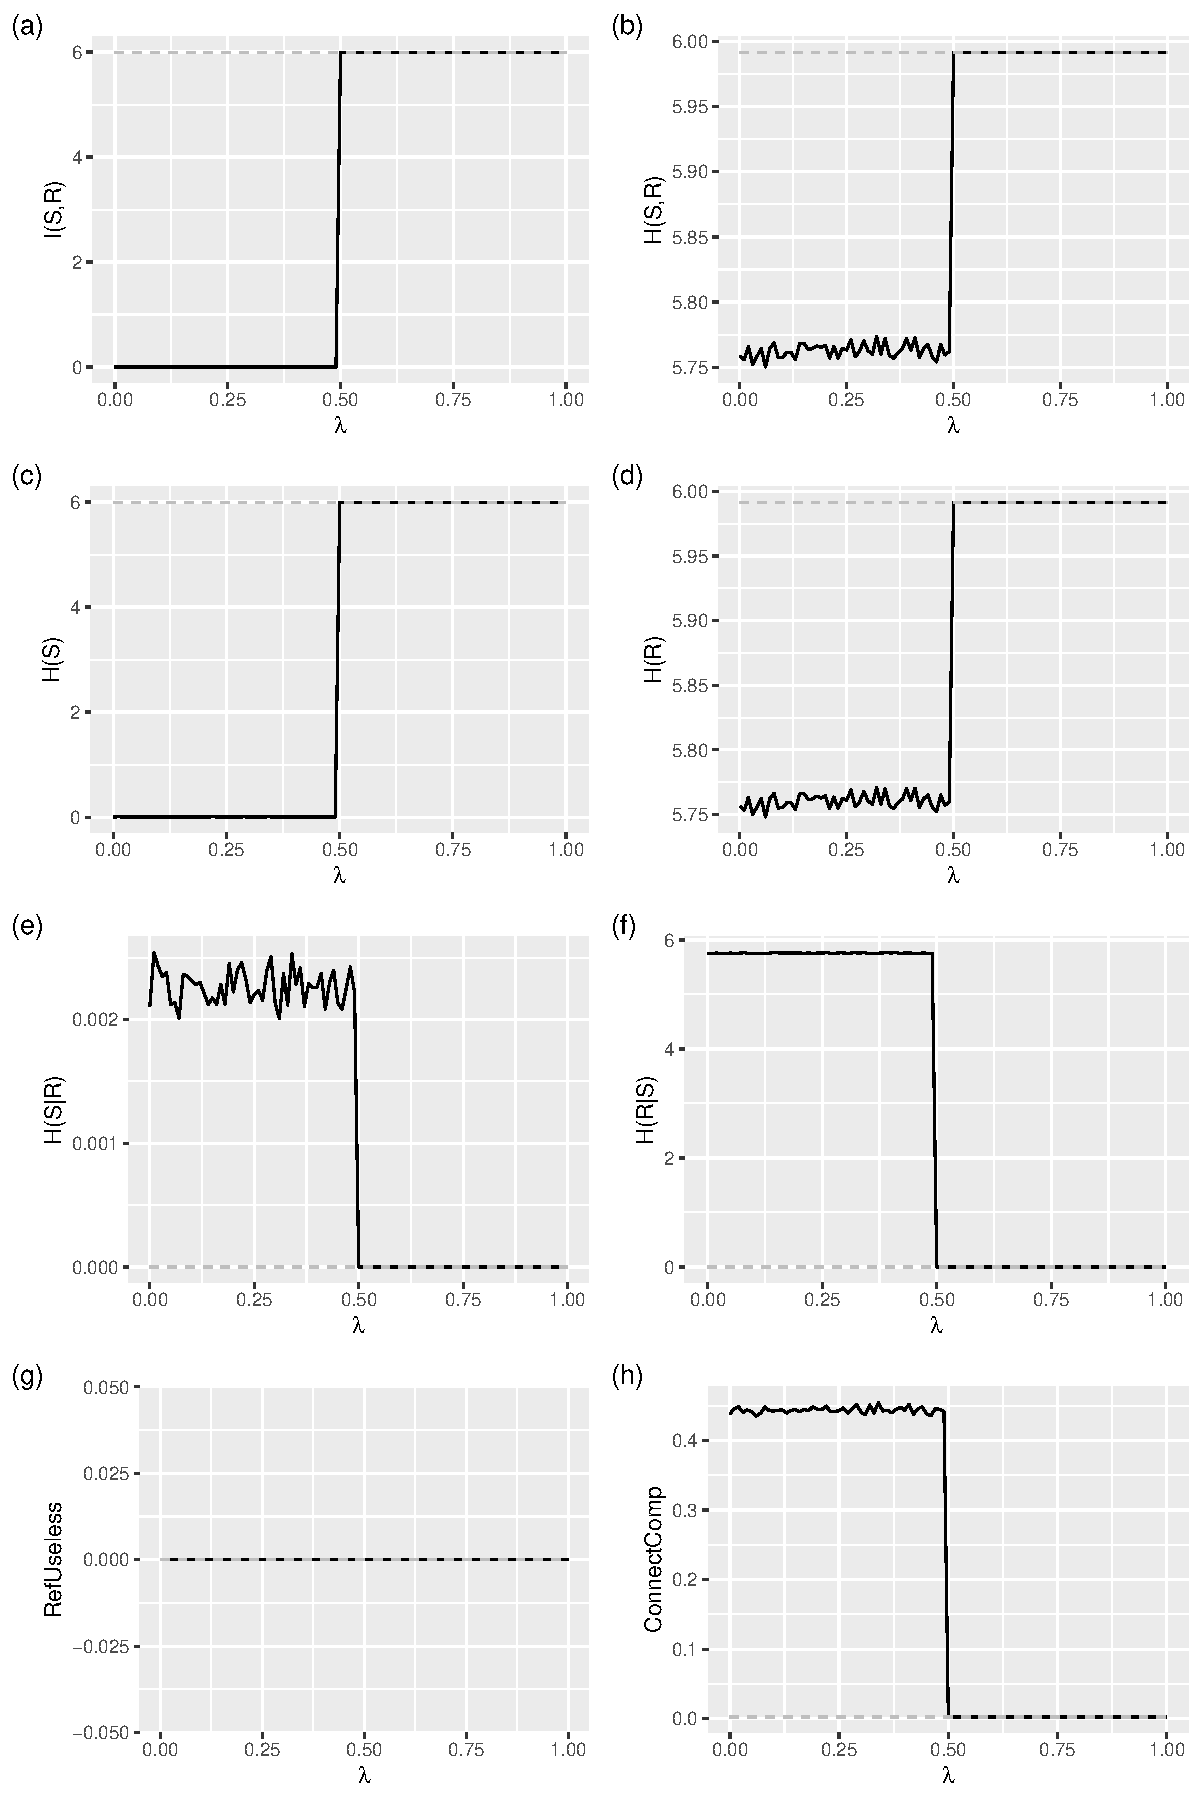
\includegraphics[width=\textwidth]{informationTheoretic_uniform_phi1_nm400_dynamic_oneToOne_allowUnlinked}
  \caption{a}
  \label{fig:informationTheoretic_uniform_phi1_nm400_dynamic_oneToOne_allowUnlinked}
\end{figure}

Figures \ref{fig:insideLambda_uniform_phi0_nm400_dynamic_randomBipartite_allowUnlinked} and \ref{fig:insideLambda_uniform_phi0_nm400_dynamic_oneToOne_allowUnlinked} (random and one-to-one respectively) show statistical measures of select values of $\lambda$, with Figures \ref{fig:fitting_insideLambda_uniform_phi0_nm400_dynamic_randomBipartite_allowUnlinked} and \ref{fig:fitting_insideLambda_uniform_phi0_nm400_dynamic_oneToOne_allowUnlinked} (random and one-to-one respectively) showing the fitting of the curve to a power law for a single select value of $\lambda$ and Tables \ref{tab:fitting_insideLambda_uniform_phi0_nm400_dynamic_randomBipartite_allowUnlinked} and \ref{tab:fitting_insideLambda_uniform_phi0_nm400_dynamic_oneToOne_allowUnlinked} (random and one-to-one respectively) showing the values of the regression exponent and factor.
As with others, the single link initial condition is not plotted for select values of $\lambda$ as it fails to evolve beyond the single link state.
Appendix \ref{sec:app_figures_second-model} shows the same figures but with disconnected meanings disallowed.



Figures \ref{fig:insideLambda_uniform_phi1_nm400_dynamic_randomBipartite_allowUnlinked}, \ref{fig:insideLambda_uniform_phi1_nm400_dynamic_singleLink_allowUnlinked} and \ref{fig:insideLambda_uniform_phi1_nm400_dynamic_oneToOne_allowUnlinked} also show statistical measures of select values of $\lambda$.
They correspond to the same initial conditions.

\begin{figure}
  \centering
  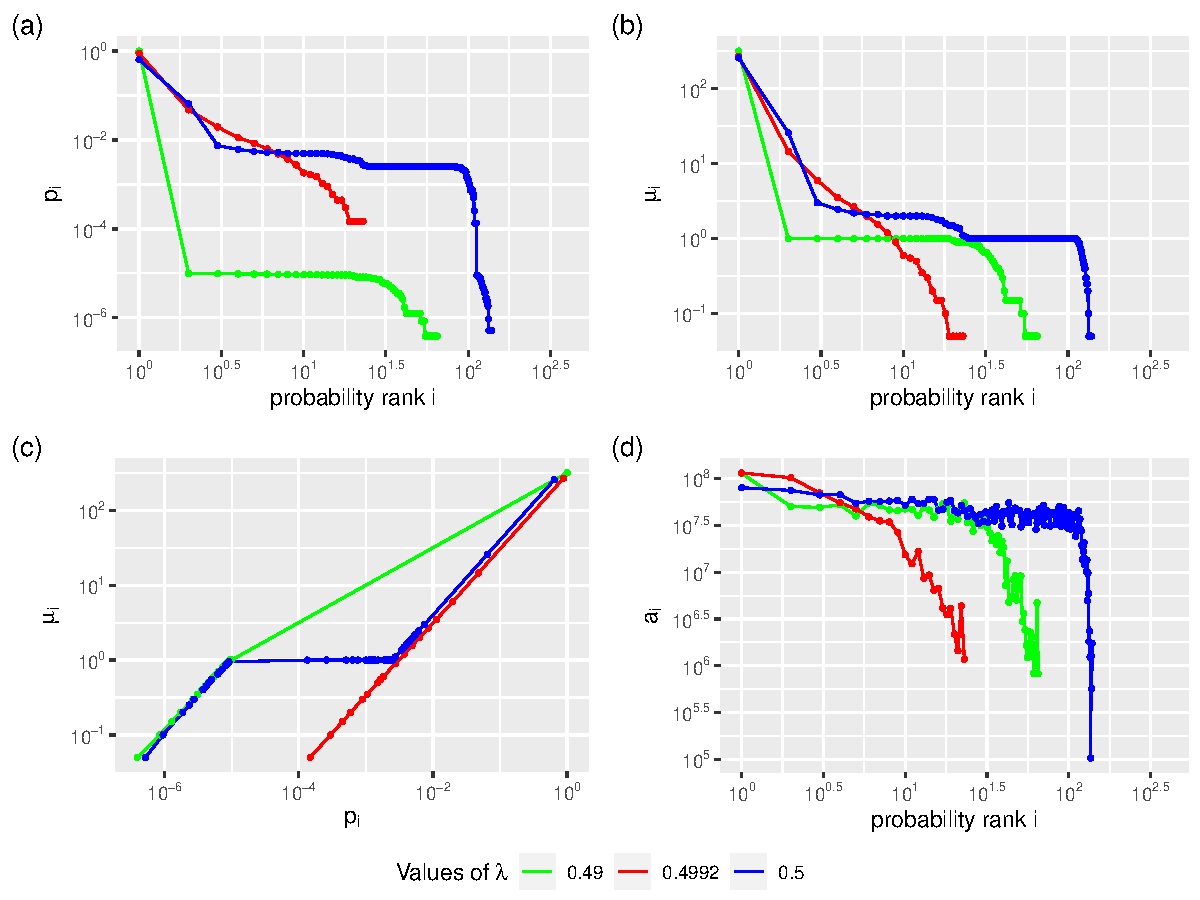
\includegraphics[width=\textwidth,draft]{insideLambda_uniform_phi1_nm400_dynamic_randomBipartite_allowUnlinked.pdf}
  \caption{a}
  \label{fig:insideLambda_uniform_phi1_nm400_dynamic_randomBipartite_allowUnlinked}
\end{figure}

\begin{figure}
  \centering
  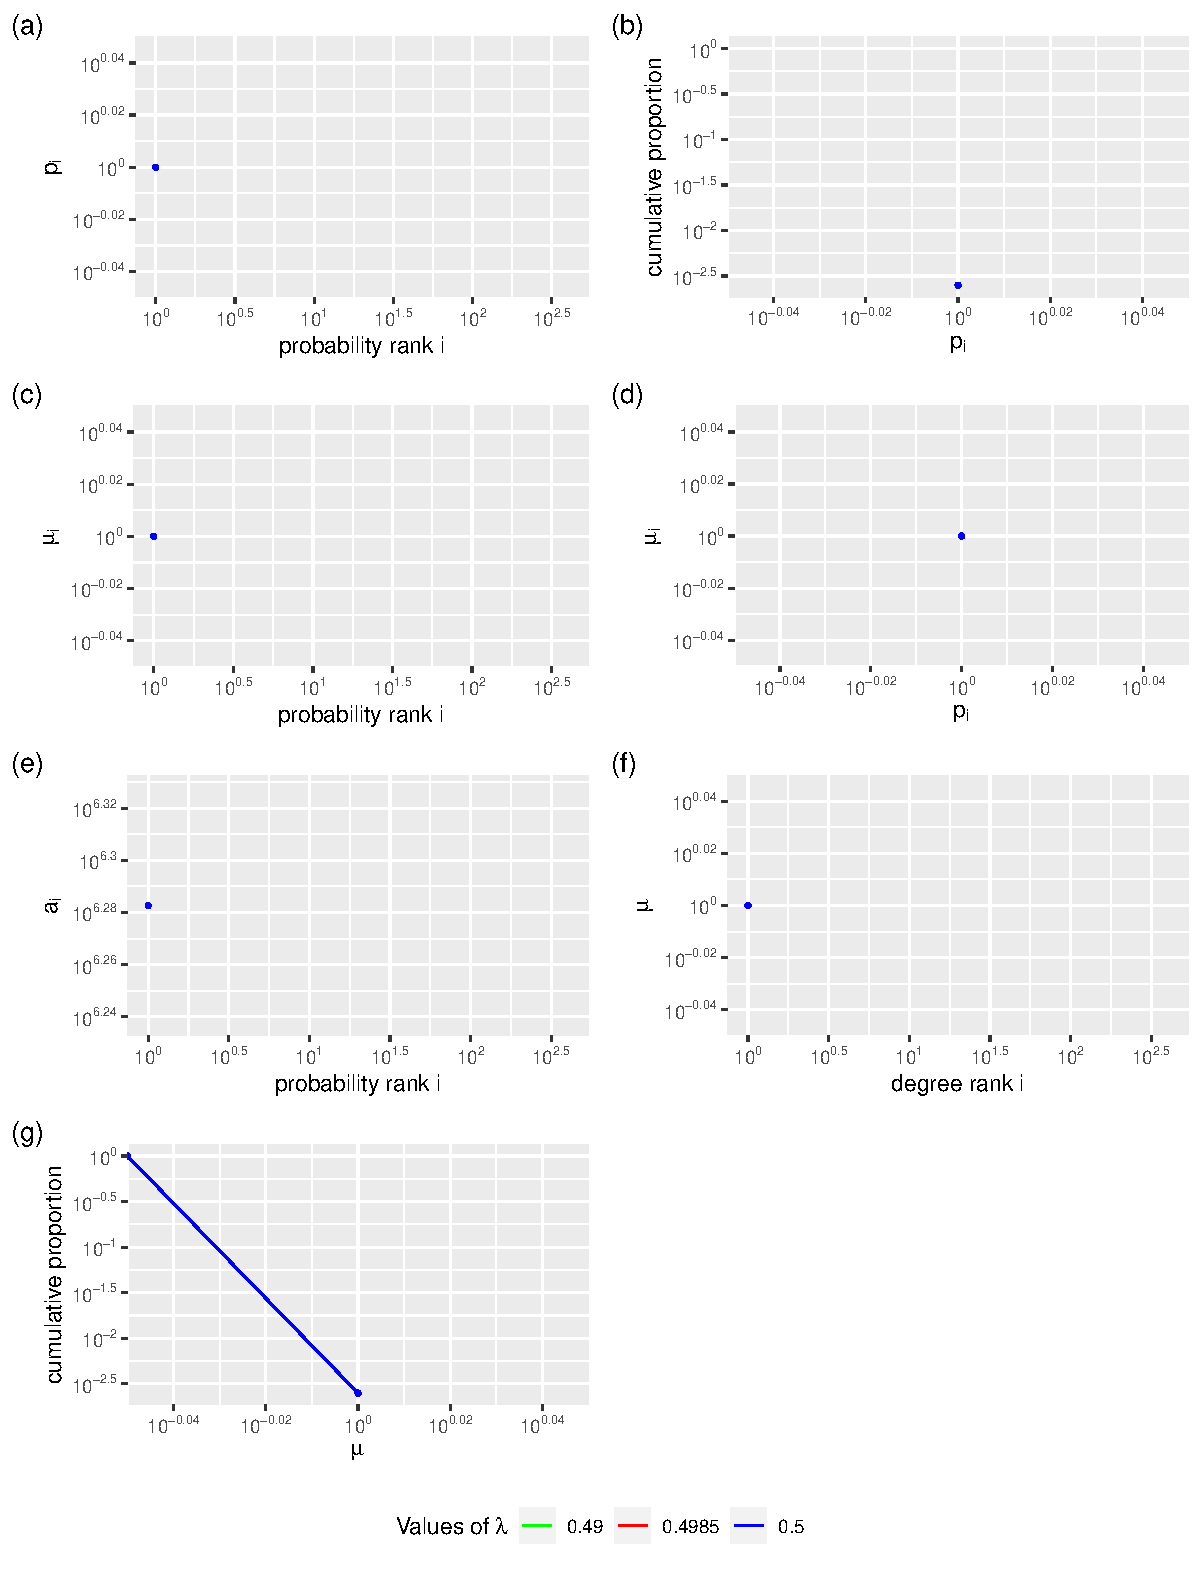
\includegraphics[width=\textwidth,draft]{insideLambda_uniform_phi1_nm400_dynamic_singleLink_allowUnlinked.pdf}
  \caption{a}
  \label{fig:insideLambda_uniform_phi1_nm400_dynamic_singleLink_allowUnlinked}
\end{figure}

\begin{figure}
  \centering
  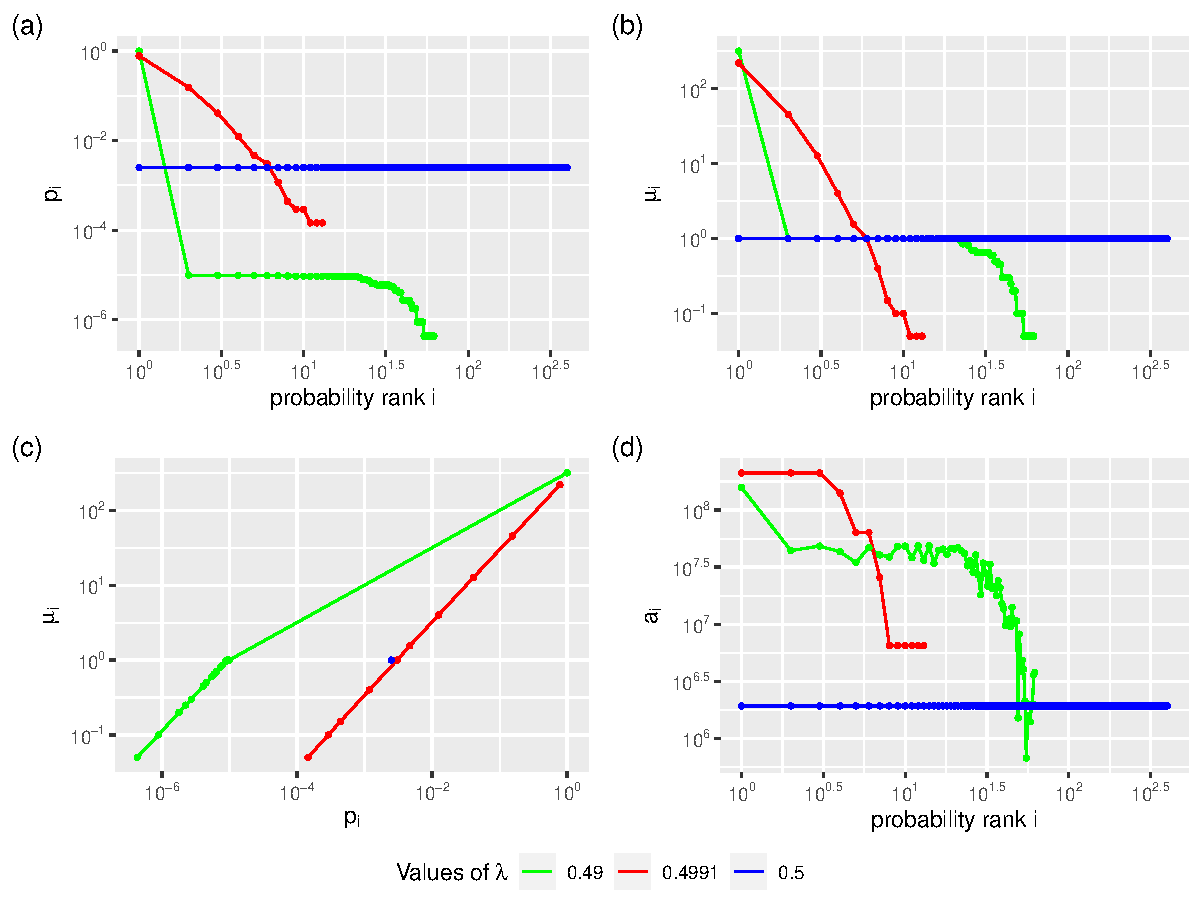
\includegraphics[width=\textwidth,draft]{insideLambda_uniform_phi1_nm400_dynamic_oneToOne_allowUnlinked.pdf}
  \caption{a}
  \label{fig:insideLambda_uniform_phi1_nm400_dynamic_oneToOne_allowUnlinked}
\end{figure}

%%% Local Variables:
%%% mode: latex
%%% TeX-master: "tfm"
%%% End:
